\documentclass[twoside]{book}

% Packages required by doxygen
\usepackage{calc}
\usepackage{doxygen}
\usepackage{graphicx}
\usepackage[utf8]{inputenc}
\usepackage{makeidx}
\usepackage{multicol}
\usepackage{multirow}
\usepackage{fixltx2e}
\PassOptionsToPackage{warn}{textcomp}
\usepackage{textcomp}
\usepackage[nointegrals]{wasysym}
\usepackage[table]{xcolor}

% Font selection
\usepackage[T1]{fontenc}
\usepackage{mathptmx}
\usepackage[scaled=.90]{helvet}
\usepackage{courier}
\usepackage{amssymb}
\usepackage{sectsty}
\renewcommand{\familydefault}{\sfdefault}
\allsectionsfont{%
  \fontseries{bc}\selectfont%
  \color{darkgray}%
}
\renewcommand{\DoxyLabelFont}{%
  \fontseries{bc}\selectfont%
  \color{darkgray}%
}
\newcommand{\+}{\discretionary{\mbox{\scriptsize$\hookleftarrow$}}{}{}}

% Page & text layout
\usepackage{geometry}
\geometry{%
  a4paper,%
  top=2.5cm,%
  bottom=2.5cm,%
  left=2.5cm,%
  right=2.5cm%
}
\tolerance=750
\hfuzz=15pt
\hbadness=750
\setlength{\emergencystretch}{15pt}
\setlength{\parindent}{0cm}
\setlength{\parskip}{0.2cm}
\makeatletter
\renewcommand{\paragraph}{%
  \@startsection{paragraph}{4}{0ex}{-1.0ex}{1.0ex}{%
    \normalfont\normalsize\bfseries\SS@parafont%
  }%
}
\renewcommand{\subparagraph}{%
  \@startsection{subparagraph}{5}{0ex}{-1.0ex}{1.0ex}{%
    \normalfont\normalsize\bfseries\SS@subparafont%
  }%
}
\makeatother

% Headers & footers
\usepackage{fancyhdr}
\pagestyle{fancyplain}
\fancyhead[LE]{\fancyplain{}{\bfseries\thepage}}
\fancyhead[CE]{\fancyplain{}{}}
\fancyhead[RE]{\fancyplain{}{\bfseries\leftmark}}
\fancyhead[LO]{\fancyplain{}{\bfseries\rightmark}}
\fancyhead[CO]{\fancyplain{}{}}
\fancyhead[RO]{\fancyplain{}{\bfseries\thepage}}
\fancyfoot[LE]{\fancyplain{}{}}
\fancyfoot[CE]{\fancyplain{}{}}
\fancyfoot[RE]{\fancyplain{}{\bfseries\scriptsize Generated on Tue Jan 12 2016 13\+:57\+:08 for Z\+L\+Util by Doxygen }}
\fancyfoot[LO]{\fancyplain{}{\bfseries\scriptsize Generated on Tue Jan 12 2016 13\+:57\+:08 for Z\+L\+Util by Doxygen }}
\fancyfoot[CO]{\fancyplain{}{}}
\fancyfoot[RO]{\fancyplain{}{}}
\renewcommand{\footrulewidth}{0.4pt}
\renewcommand{\chaptermark}[1]{%
  \markboth{#1}{}%
}
\renewcommand{\sectionmark}[1]{%
  \markright{\thesection\ #1}%
}

% Indices & bibliography
\usepackage{natbib}
\usepackage[titles]{tocloft}
\setcounter{tocdepth}{3}
\setcounter{secnumdepth}{5}
\makeindex

% Hyperlinks (required, but should be loaded last)
\usepackage{ifpdf}
\ifpdf
  \usepackage[pdftex,pagebackref=true]{hyperref}
\else
  \usepackage[ps2pdf,pagebackref=true]{hyperref}
\fi
\hypersetup{%
  colorlinks=true,%
  linkcolor=blue,%
  citecolor=blue,%
  unicode%
}

% Custom commands
\newcommand{\clearemptydoublepage}{%
  \newpage{\pagestyle{empty}\cleardoublepage}%
}


%===== C O N T E N T S =====

\begin{document}

% Titlepage & ToC
\hypersetup{pageanchor=false,
             bookmarks=true,
             bookmarksnumbered=true,
             pdfencoding=unicode
            }
\pagenumbering{roman}
\begin{titlepage}
\vspace*{7cm}
\begin{center}%
{\Large Z\+L\+Util }\\
\vspace*{1cm}
{\large Generated by Doxygen 1.8.7}\\
\vspace*{0.5cm}
{\small Tue Jan 12 2016 13:57:08}\\
\end{center}
\end{titlepage}
\clearemptydoublepage
\tableofcontents
\clearemptydoublepage
\pagenumbering{arabic}
\hypersetup{pageanchor=true}

%--- Begin generated contents ---
\chapter{Z\+L\+Util}
\label{md__r_e_a_d_m_e}
\hypertarget{md__r_e_a_d_m_e}{}
Z\+L\+Util provide common used function. For personal project use. 
\chapter{Deprecated List}
\label{deprecated}
\hypertarget{deprecated}{}

\begin{DoxyRefList}
\item[\label{deprecated__deprecated000001}%
\hypertarget{deprecated__deprecated000001}{}%
Member \hyperlink{interface_util_a344afa0140847ec221b1dbbcb04687f3}{\mbox{[}Util is\+Network\+Available\mbox{]}} ]直接使用\mbox{[}\mbox{[}Cloud\+Client shared\+Instance\mbox{]} is\+Reachable\mbox{]}; \begin{DoxyReturn}{Returns}

\end{DoxyReturn}

\end{DoxyRefList}
\chapter{Hierarchical Index}
\section{Class Hierarchy}
This inheritance list is sorted roughly, but not completely, alphabetically\+:\begin{DoxyCompactList}
\item \contentsline{section}{G\+Data\+X\+M\+L\+Document(Private\+Methods)}{\pageref{category_g_data_x_m_l_document_07_private_methods_08}}{}
\item \contentsline{section}{G\+Data\+X\+M\+L\+Element(Private\+Methods)}{\pageref{category_g_data_x_m_l_element_07_private_methods_08}}{}
\item \contentsline{section}{G\+Data\+X\+M\+L\+Node(Private\+Methods)}{\pageref{category_g_data_x_m_l_node_07_private_methods_08}}{}
\item \contentsline{section}{J\+K\+Buffer}{\pageref{struct_j_k_buffer}}{}
\item \contentsline{section}{J\+K\+Const\+Buffer}{\pageref{struct_j_k_const_buffer}}{}
\item \contentsline{section}{J\+K\+Const\+Ptr\+Range}{\pageref{struct_j_k_const_ptr_range}}{}
\item \contentsline{section}{J\+K\+Encode\+Cache}{\pageref{struct_j_k_encode_cache}}{}
\item \contentsline{section}{J\+K\+Encode\+State}{\pageref{struct_j_k_encode_state}}{}
\item \contentsline{section}{J\+K\+Fast\+Class\+Lookup}{\pageref{struct_j_k_fast_class_lookup}}{}
\item \contentsline{section}{J\+K\+Hash\+Table\+Entry}{\pageref{struct_j_k_hash_table_entry}}{}
\item \contentsline{section}{J\+K\+Managed\+Buffer}{\pageref{struct_j_k_managed_buffer}}{}
\item \contentsline{section}{J\+K\+Obj\+C\+Imp\+Cache}{\pageref{struct_j_k_obj_c_imp_cache}}{}
\item \contentsline{section}{J\+K\+Object\+Stack}{\pageref{struct_j_k_object_stack}}{}
\item \contentsline{section}{J\+K\+Parse\+State}{\pageref{struct_j_k_parse_state}}{}
\item \contentsline{section}{J\+K\+Parse\+Token}{\pageref{struct_j_k_parse_token}}{}
\item \contentsline{section}{J\+K\+Ptr\+Range}{\pageref{struct_j_k_ptr_range}}{}
\item \contentsline{section}{J\+K\+Range}{\pageref{struct_j_k_range}}{}
\item \contentsline{section}{J\+K\+Token\+Cache}{\pageref{struct_j_k_token_cache}}{}
\item \contentsline{section}{J\+K\+Token\+Cache\+Item}{\pageref{struct_j_k_token_cache_item}}{}
\item \contentsline{section}{J\+K\+Token\+Value}{\pageref{struct_j_k_token_value}}{}
\item \contentsline{section}{J\+S\+O\+N\+Decoder}{\pageref{class_j_s_o_n_decoder}}{}
\item \contentsline{section}{M\+K\+Number\+Badge\+View()}{\pageref{category_m_k_number_badge_view_07_08}}{}
\item \contentsline{section}{N\+S\+Array(J\+S\+O\+N\+Kit\+Serializing)}{\pageref{category_n_s_array_07_j_s_o_n_kit_serializing_08}}{}
\item $<$N\+S\+Copying$>$\begin{DoxyCompactList}
\item \contentsline{section}{G\+Data\+X\+M\+L\+Node}{\pageref{interface_g_data_x_m_l_node}}{}
\begin{DoxyCompactList}
\item \contentsline{section}{G\+Data\+X\+M\+L\+Element}{\pageref{interface_g_data_x_m_l_element}}{}
\end{DoxyCompactList}
\item \contentsline{section}{J\+K\+Array}{\pageref{interface_j_k_array}}{}
\item \contentsline{section}{J\+K\+Dictionary}{\pageref{interface_j_k_dictionary}}{}
\end{DoxyCompactList}
\item \contentsline{section}{N\+S\+Data(Compressor)}{\pageref{category_n_s_data_07_compressor_08}}{}
\item \contentsline{section}{N\+S\+Data(Encryption)}{\pageref{category_n_s_data_07_encryption_08}}{}
\item \contentsline{section}{N\+S\+Data(J\+S\+O\+N\+Kit\+Deserializing)}{\pageref{category_n_s_data_07_j_s_o_n_kit_deserializing_08}}{}
\item \contentsline{section}{N\+S\+Dictionary(Dictionary2\+J\+S\+O\+N)}{\pageref{category_n_s_dictionary_07_dictionary2_j_s_o_n_08}}{}
\item \contentsline{section}{N\+S\+Dictionary(J\+S\+O\+N\+Kit\+Serializing)}{\pageref{category_n_s_dictionary_07_j_s_o_n_kit_serializing_08}}{}
\item N\+S\+Enumerator\begin{DoxyCompactList}
\item \contentsline{section}{J\+K\+Dictionary\+Enumerator}{\pageref{interface_j_k_dictionary_enumerator}}{}
\end{DoxyCompactList}
\item $<$N\+S\+Fast\+Enumeration$>$\begin{DoxyCompactList}
\item \contentsline{section}{J\+K\+Array}{\pageref{interface_j_k_array}}{}
\item \contentsline{section}{J\+K\+Dictionary}{\pageref{interface_j_k_dictionary}}{}
\end{DoxyCompactList}
\item N\+S\+Mutable\+Array\begin{DoxyCompactList}
\item \contentsline{section}{J\+K\+Array}{\pageref{interface_j_k_array}}{}
\end{DoxyCompactList}
\item $<$N\+S\+Mutable\+Copying$>$\begin{DoxyCompactList}
\item \contentsline{section}{J\+K\+Array}{\pageref{interface_j_k_array}}{}
\item \contentsline{section}{J\+K\+Dictionary}{\pageref{interface_j_k_dictionary}}{}
\end{DoxyCompactList}
\item N\+S\+Mutable\+Dictionary\begin{DoxyCompactList}
\item \contentsline{section}{J\+K\+Dictionary}{\pageref{interface_j_k_dictionary}}{}
\end{DoxyCompactList}
\item N\+S\+Object\begin{DoxyCompactList}
\item \contentsline{section}{Core\+Data\+Manager}{\pageref{interface_core_data_manager}}{}
\item \contentsline{section}{G\+Data\+X\+M\+L\+Document}{\pageref{interface_g_data_x_m_l_document}}{}
\item \contentsline{section}{G\+Data\+X\+M\+L\+Node}{\pageref{interface_g_data_x_m_l_node}}{}
\item \contentsline{section}{J\+K\+Serializer}{\pageref{interface_j_k_serializer}}{}
\item \contentsline{section}{Util}{\pageref{interface_util}}{}
\end{DoxyCompactList}
\item \contentsline{section}{N\+S\+Object(Class\+Name)}{\pageref{category_n_s_object_07_class_name_08}}{}
\item \contentsline{section}{N\+S\+String(A\+E\+S256\+Encrypt)}{\pageref{category_n_s_string_07_a_e_s256_encrypt_08}}{}
\item \contentsline{section}{N\+S\+String(J\+S\+O\+N\+Kit\+Deserializing)}{\pageref{category_n_s_string_07_j_s_o_n_kit_deserializing_08}}{}
\item \contentsline{section}{N\+S\+String(J\+S\+O\+N\+Kit\+Serializing)}{\pageref{category_n_s_string_07_j_s_o_n_kit_serializing_08}}{}
\item \contentsline{section}{N\+S\+String(Trim)}{\pageref{category_n_s_string_07_trim_08}}{}
\item \contentsline{section}{N\+S\+String(U\+R\+L)}{\pageref{category_n_s_string_07_u_r_l_08}}{}
\item \contentsline{section}{U\+I\+Alert\+View(Block)}{\pageref{category_u_i_alert_view_07_block_08}}{}
\item U\+I\+Button\begin{DoxyCompactList}
\item \contentsline{section}{Z\+L\+Object\+Button}{\pageref{interface_z_l_object_button}}{}
\item \contentsline{section}{Z\+L\+Object\+Button}{\pageref{interface_z_l_object_button}}{}
\end{DoxyCompactList}
\item \contentsline{section}{U\+I\+Color(U\+I\+Color\+From\+Hex)}{\pageref{category_u_i_color_07_u_i_color_from_hex_08}}{}
\item \contentsline{section}{U\+I\+Image(Circle\+Image)}{\pageref{category_u_i_image_07_circle_image_08}}{}
\item \contentsline{section}{U\+I\+Image(U\+I\+Image\+From\+U\+I\+Color)}{\pageref{category_u_i_image_07_u_i_image_from_u_i_color_08}}{}
\item \contentsline{section}{U\+I\+Image(U\+I\+Rounded\+Rect\+Image)}{\pageref{category_u_i_image_07_u_i_rounded_rect_image_08}}{}
\item \contentsline{section}{U\+I\+Navigation\+Bar(Customize)}{\pageref{category_u_i_navigation_bar_07_customize_08}}{}
\item \contentsline{section}{U\+I\+Tab\+Bar(Customize)}{\pageref{category_u_i_tab_bar_07_customize_08}}{}
\item U\+I\+Text\+Field\begin{DoxyCompactList}
\item \contentsline{section}{Z\+L\+Object\+Text\+Field}{\pageref{interface_z_l_object_text_field}}{}
\item \contentsline{section}{Z\+L\+Object\+Text\+Field}{\pageref{interface_z_l_object_text_field}}{}
\end{DoxyCompactList}
\item U\+I\+View\begin{DoxyCompactList}
\item \contentsline{section}{M\+K\+Number\+Badge\+View}{\pageref{interface_m_k_number_badge_view}}{}
\end{DoxyCompactList}
\item \contentsline{section}{U\+I\+View(H\+K\+Project\+Base)}{\pageref{category_u_i_view_07_h_k_project_base_08}}{}
\item \contentsline{section}{U\+I\+View(Update\+Frame)}{\pageref{category_u_i_view_07_update_frame_08}}{}
\item \contentsline{section}{Z\+L\+G\+T\+M\+Base64}{\pageref{class_z_l_g_t_m_base64}}{}
\item \contentsline{section}{Z\+L\+G\+T\+M\+Base64(Private\+Methods)}{\pageref{category_z_l_g_t_m_base64_07_private_methods_08}}{}
\end{DoxyCompactList}

\chapter{Class Index}
\section{Class List}
Here are the classes, structs, unions and interfaces with brief descriptions\+:\begin{DoxyCompactList}
\item\contentsline{section}{\hyperlink{interface_core_data_manager}{Core\+Data\+Manager} }{\pageref{interface_core_data_manager}}{}
\item\contentsline{section}{\hyperlink{interface_g_data_x_m_l_document}{G\+Data\+X\+M\+L\+Document} }{\pageref{interface_g_data_x_m_l_document}}{}
\item\contentsline{section}{\hyperlink{category_g_data_x_m_l_document_07_private_methods_08}{G\+Data\+X\+M\+L\+Document(\+Private\+Methods)} }{\pageref{category_g_data_x_m_l_document_07_private_methods_08}}{}
\item\contentsline{section}{\hyperlink{interface_g_data_x_m_l_element}{G\+Data\+X\+M\+L\+Element} }{\pageref{interface_g_data_x_m_l_element}}{}
\item\contentsline{section}{\hyperlink{category_g_data_x_m_l_element_07_private_methods_08}{G\+Data\+X\+M\+L\+Element(\+Private\+Methods)} }{\pageref{category_g_data_x_m_l_element_07_private_methods_08}}{}
\item\contentsline{section}{\hyperlink{interface_g_data_x_m_l_node}{G\+Data\+X\+M\+L\+Node} }{\pageref{interface_g_data_x_m_l_node}}{}
\item\contentsline{section}{\hyperlink{category_g_data_x_m_l_node_07_private_methods_08}{G\+Data\+X\+M\+L\+Node(\+Private\+Methods)} }{\pageref{category_g_data_x_m_l_node_07_private_methods_08}}{}
\item\contentsline{section}{\hyperlink{interface_j_k_array}{J\+K\+Array} }{\pageref{interface_j_k_array}}{}
\item\contentsline{section}{\hyperlink{struct_j_k_buffer}{J\+K\+Buffer} }{\pageref{struct_j_k_buffer}}{}
\item\contentsline{section}{\hyperlink{struct_j_k_const_buffer}{J\+K\+Const\+Buffer} }{\pageref{struct_j_k_const_buffer}}{}
\item\contentsline{section}{\hyperlink{struct_j_k_const_ptr_range}{J\+K\+Const\+Ptr\+Range} }{\pageref{struct_j_k_const_ptr_range}}{}
\item\contentsline{section}{\hyperlink{interface_j_k_dictionary}{J\+K\+Dictionary} }{\pageref{interface_j_k_dictionary}}{}
\item\contentsline{section}{\hyperlink{interface_j_k_dictionary_enumerator}{J\+K\+Dictionary\+Enumerator} }{\pageref{interface_j_k_dictionary_enumerator}}{}
\item\contentsline{section}{\hyperlink{struct_j_k_encode_cache}{J\+K\+Encode\+Cache} }{\pageref{struct_j_k_encode_cache}}{}
\item\contentsline{section}{\hyperlink{struct_j_k_encode_state}{J\+K\+Encode\+State} }{\pageref{struct_j_k_encode_state}}{}
\item\contentsline{section}{\hyperlink{struct_j_k_fast_class_lookup}{J\+K\+Fast\+Class\+Lookup} }{\pageref{struct_j_k_fast_class_lookup}}{}
\item\contentsline{section}{\hyperlink{struct_j_k_hash_table_entry}{J\+K\+Hash\+Table\+Entry} }{\pageref{struct_j_k_hash_table_entry}}{}
\item\contentsline{section}{\hyperlink{struct_j_k_managed_buffer}{J\+K\+Managed\+Buffer} }{\pageref{struct_j_k_managed_buffer}}{}
\item\contentsline{section}{\hyperlink{struct_j_k_obj_c_imp_cache}{J\+K\+Obj\+C\+Imp\+Cache} }{\pageref{struct_j_k_obj_c_imp_cache}}{}
\item\contentsline{section}{\hyperlink{struct_j_k_object_stack}{J\+K\+Object\+Stack} }{\pageref{struct_j_k_object_stack}}{}
\item\contentsline{section}{\hyperlink{struct_j_k_parse_state}{J\+K\+Parse\+State} }{\pageref{struct_j_k_parse_state}}{}
\item\contentsline{section}{\hyperlink{struct_j_k_parse_token}{J\+K\+Parse\+Token} }{\pageref{struct_j_k_parse_token}}{}
\item\contentsline{section}{\hyperlink{struct_j_k_ptr_range}{J\+K\+Ptr\+Range} }{\pageref{struct_j_k_ptr_range}}{}
\item\contentsline{section}{\hyperlink{struct_j_k_range}{J\+K\+Range} }{\pageref{struct_j_k_range}}{}
\item\contentsline{section}{\hyperlink{interface_j_k_serializer}{J\+K\+Serializer} }{\pageref{interface_j_k_serializer}}{}
\item\contentsline{section}{\hyperlink{struct_j_k_token_cache}{J\+K\+Token\+Cache} }{\pageref{struct_j_k_token_cache}}{}
\item\contentsline{section}{\hyperlink{struct_j_k_token_cache_item}{J\+K\+Token\+Cache\+Item} }{\pageref{struct_j_k_token_cache_item}}{}
\item\contentsline{section}{\hyperlink{struct_j_k_token_value}{J\+K\+Token\+Value} }{\pageref{struct_j_k_token_value}}{}
\item\contentsline{section}{\hyperlink{class_j_s_o_n_decoder}{J\+S\+O\+N\+Decoder} }{\pageref{class_j_s_o_n_decoder}}{}
\item\contentsline{section}{\hyperlink{interface_m_k_number_badge_view}{M\+K\+Number\+Badge\+View} }{\pageref{interface_m_k_number_badge_view}}{}
\item\contentsline{section}{\hyperlink{category_m_k_number_badge_view_07_08}{M\+K\+Number\+Badge\+View()} }{\pageref{category_m_k_number_badge_view_07_08}}{}
\item\contentsline{section}{\hyperlink{category_n_s_array_07_j_s_o_n_kit_serializing_08}{N\+S\+Array(\+J\+S\+O\+N\+Kit\+Serializing)} }{\pageref{category_n_s_array_07_j_s_o_n_kit_serializing_08}}{}
\item\contentsline{section}{\hyperlink{category_n_s_data_07_compressor_08}{N\+S\+Data(\+Compressor)} }{\pageref{category_n_s_data_07_compressor_08}}{}
\item\contentsline{section}{\hyperlink{category_n_s_data_07_encryption_08}{N\+S\+Data(\+Encryption)} }{\pageref{category_n_s_data_07_encryption_08}}{}
\item\contentsline{section}{\hyperlink{category_n_s_data_07_j_s_o_n_kit_deserializing_08}{N\+S\+Data(\+J\+S\+O\+N\+Kit\+Deserializing)} }{\pageref{category_n_s_data_07_j_s_o_n_kit_deserializing_08}}{}
\item\contentsline{section}{\hyperlink{category_n_s_dictionary_07_dictionary2_j_s_o_n_08}{N\+S\+Dictionary(\+Dictionary2\+J\+S\+O\+N)} }{\pageref{category_n_s_dictionary_07_dictionary2_j_s_o_n_08}}{}
\item\contentsline{section}{\hyperlink{category_n_s_dictionary_07_j_s_o_n_kit_serializing_08}{N\+S\+Dictionary(\+J\+S\+O\+N\+Kit\+Serializing)} }{\pageref{category_n_s_dictionary_07_j_s_o_n_kit_serializing_08}}{}
\item\contentsline{section}{\hyperlink{category_n_s_object_07_class_name_08}{N\+S\+Object(\+Class\+Name)} }{\pageref{category_n_s_object_07_class_name_08}}{}
\item\contentsline{section}{\hyperlink{category_n_s_string_07_a_e_s256_encrypt_08}{N\+S\+String(\+A\+E\+S256\+Encrypt)} }{\pageref{category_n_s_string_07_a_e_s256_encrypt_08}}{}
\item\contentsline{section}{\hyperlink{category_n_s_string_07_j_s_o_n_kit_deserializing_08}{N\+S\+String(\+J\+S\+O\+N\+Kit\+Deserializing)} }{\pageref{category_n_s_string_07_j_s_o_n_kit_deserializing_08}}{}
\item\contentsline{section}{\hyperlink{category_n_s_string_07_j_s_o_n_kit_serializing_08}{N\+S\+String(\+J\+S\+O\+N\+Kit\+Serializing)} }{\pageref{category_n_s_string_07_j_s_o_n_kit_serializing_08}}{}
\item\contentsline{section}{\hyperlink{category_n_s_string_07_trim_08}{N\+S\+String(\+Trim)} }{\pageref{category_n_s_string_07_trim_08}}{}
\item\contentsline{section}{\hyperlink{category_n_s_string_07_u_r_l_08}{N\+S\+String(\+U\+R\+L)} }{\pageref{category_n_s_string_07_u_r_l_08}}{}
\item\contentsline{section}{\hyperlink{category_u_i_alert_view_07_block_08}{U\+I\+Alert\+View(\+Block)} }{\pageref{category_u_i_alert_view_07_block_08}}{}
\item\contentsline{section}{\hyperlink{category_u_i_color_07_u_i_color_from_hex_08}{U\+I\+Color(\+U\+I\+Color\+From\+Hex)} }{\pageref{category_u_i_color_07_u_i_color_from_hex_08}}{}
\item\contentsline{section}{\hyperlink{category_u_i_image_07_circle_image_08}{U\+I\+Image(\+Circle\+Image)} }{\pageref{category_u_i_image_07_circle_image_08}}{}
\item\contentsline{section}{\hyperlink{category_u_i_image_07_u_i_image_from_u_i_color_08}{U\+I\+Image(\+U\+I\+Image\+From\+U\+I\+Color)} }{\pageref{category_u_i_image_07_u_i_image_from_u_i_color_08}}{}
\item\contentsline{section}{\hyperlink{category_u_i_image_07_u_i_rounded_rect_image_08}{U\+I\+Image(\+U\+I\+Rounded\+Rect\+Image)} }{\pageref{category_u_i_image_07_u_i_rounded_rect_image_08}}{}
\item\contentsline{section}{\hyperlink{category_u_i_navigation_bar_07_customize_08}{U\+I\+Navigation\+Bar(\+Customize)} }{\pageref{category_u_i_navigation_bar_07_customize_08}}{}
\item\contentsline{section}{\hyperlink{category_u_i_tab_bar_07_customize_08}{U\+I\+Tab\+Bar(\+Customize)} }{\pageref{category_u_i_tab_bar_07_customize_08}}{}
\item\contentsline{section}{\hyperlink{category_u_i_view_07_h_k_project_base_08}{U\+I\+View(\+H\+K\+Project\+Base)} }{\pageref{category_u_i_view_07_h_k_project_base_08}}{}
\item\contentsline{section}{\hyperlink{category_u_i_view_07_update_frame_08}{U\+I\+View(\+Update\+Frame)} }{\pageref{category_u_i_view_07_update_frame_08}}{}
\item\contentsline{section}{\hyperlink{interface_util}{Util} }{\pageref{interface_util}}{}
\item\contentsline{section}{\hyperlink{class_z_l_g_t_m_base64}{Z\+L\+G\+T\+M\+Base64} }{\pageref{class_z_l_g_t_m_base64}}{}
\item\contentsline{section}{\hyperlink{category_z_l_g_t_m_base64_07_private_methods_08}{Z\+L\+G\+T\+M\+Base64(\+Private\+Methods)} }{\pageref{category_z_l_g_t_m_base64_07_private_methods_08}}{}
\item\contentsline{section}{\hyperlink{interface_z_l_object_button}{Z\+L\+Object\+Button} }{\pageref{interface_z_l_object_button}}{}
\item\contentsline{section}{\hyperlink{interface_z_l_object_text_field}{Z\+L\+Object\+Text\+Field} }{\pageref{interface_z_l_object_text_field}}{}
\end{DoxyCompactList}

\chapter{Class Documentation}
\hypertarget{interface_core_data_manager}{\section{Core\+Data\+Manager Class Reference}
\label{interface_core_data_manager}\index{Core\+Data\+Manager@{Core\+Data\+Manager}}
}
Inheritance diagram for Core\+Data\+Manager\+:\begin{figure}[H]
\begin{center}
\leavevmode
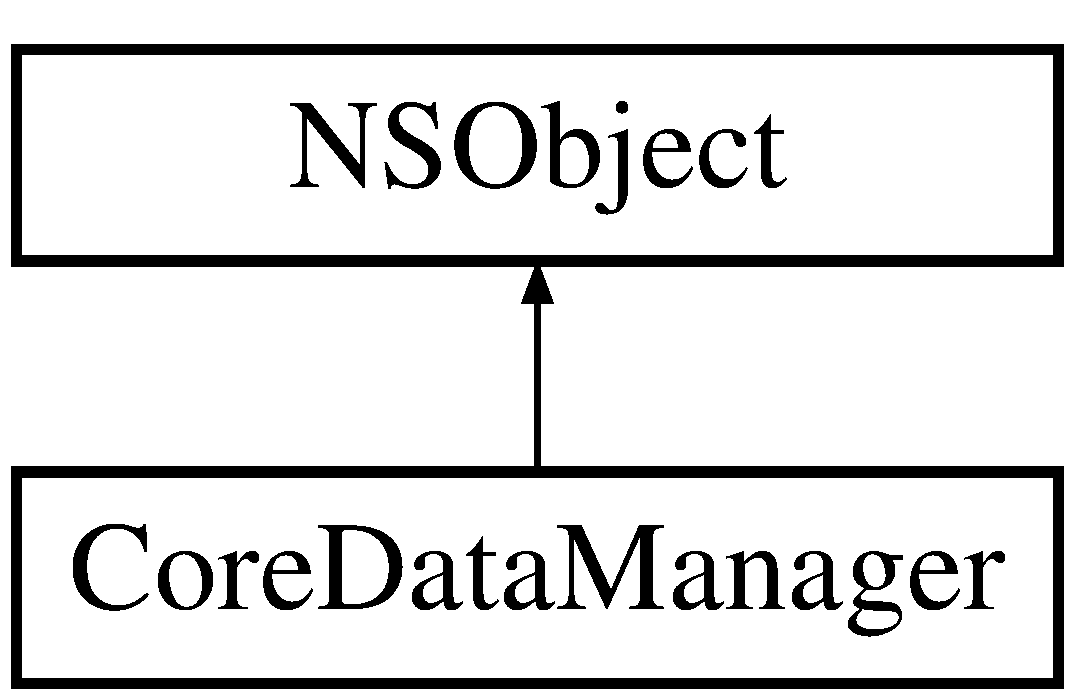
\includegraphics[height=2.000000cm]{interface_core_data_manager}
\end{center}
\end{figure}
\subsection*{Instance Methods}
\begin{DoxyCompactItemize}
\item 
(id) -\/ \hyperlink{interface_core_data_manager_ac99be2a18e096a2612cc9eafa5f88b36}{init\+With\+File\+Name\+:sqlite\+File\+Name\+:}
\item 
(N\+S\+Managed\+Object $\ast$) -\/ \hyperlink{interface_core_data_manager_a411a27a6c1fcaea2e894ffc9713fcb14}{create\+Managed\+Object\+:}
\item 
(B\+O\+O\+L) -\/ \hyperlink{interface_core_data_manager_adee944022fd4c8d45c33fe6b04b4c82f}{delete\+Managed\+Object\+:entity\+:}
\item 
(void) -\/ \hyperlink{interface_core_data_manager_a16e04f79be0510697bf6e9e0575dc33e}{delete\+All\+Objects\+:}
\item 
(N\+S\+Array $\ast$) -\/ \hyperlink{interface_core_data_manager_ac3769e057a5db88cdfdc71abc5f1f9ca}{fetch\+Managed\+Objects\+By\+Predicate\+:entity\+:sort\+Descriptors\+:}
\item 
(B\+O\+O\+L) -\/ \hyperlink{interface_core_data_manager_a0d4599a7671866520395ee195e2268c8}{save\+Context\+:}
\end{DoxyCompactItemize}
\subsection*{Class Methods}
\begin{DoxyCompactItemize}
\item 
(\hyperlink{interface_core_data_manager}{Core\+Data\+Manager} $\ast$) + \hyperlink{interface_core_data_manager_a72a3b0a316fe7508d02b8f640dc7884b}{get\+Instance}
\item 
(N\+S\+Array $\ast$) + \hyperlink{interface_core_data_manager_a4f6f5e1997e472b1a9a5b50e9410713a}{query\+:predicate\+:}
\end{DoxyCompactItemize}
\subsection*{Properties}
\begin{DoxyCompactItemize}
\item 
\hypertarget{interface_core_data_manager_ae8e3bc5409bcd4b4b16c0db274b49676}{N\+S\+Managed\+Object\+Model $\ast$ {\bfseries managed\+Object\+Model}}\label{interface_core_data_manager_ae8e3bc5409bcd4b4b16c0db274b49676}

\item 
\hypertarget{interface_core_data_manager_a04f78913860c95a80e270c6390a42211}{N\+S\+Managed\+Object\+Context $\ast$ {\bfseries managed\+Object\+Context}}\label{interface_core_data_manager_a04f78913860c95a80e270c6390a42211}

\item 
\hypertarget{interface_core_data_manager_aeb95a5451a0eb9ae52c7a94c6c01d259}{N\+S\+Persistent\+Store\+Coordinator $\ast$ {\bfseries persistent\+Store\+Coordinator}}\label{interface_core_data_manager_aeb95a5451a0eb9ae52c7a94c6c01d259}

\item 
\hypertarget{interface_core_data_manager_a2a2c49db7ffcf792775a63cf2fc9cba2}{N\+S\+String $\ast$ {\bfseries model\+File\+Name}}\label{interface_core_data_manager_a2a2c49db7ffcf792775a63cf2fc9cba2}

\item 
\hypertarget{interface_core_data_manager_ae807ce3cd077ce33dccd428eaf708721}{N\+S\+String $\ast$ {\bfseries sqlite\+File\+Name}}\label{interface_core_data_manager_ae807ce3cd077ce33dccd428eaf708721}

\end{DoxyCompactItemize}


\subsection{Method Documentation}
\hypertarget{interface_core_data_manager_a411a27a6c1fcaea2e894ffc9713fcb14}{\index{Core\+Data\+Manager@{Core\+Data\+Manager}!create\+Managed\+Object\+:@{create\+Managed\+Object\+:}}
\index{create\+Managed\+Object\+:@{create\+Managed\+Object\+:}!Core\+Data\+Manager@{Core\+Data\+Manager}}
\subsubsection[{create\+Managed\+Object\+:}]{\setlength{\rightskip}{0pt plus 5cm}-\/ (N\+S\+Managed\+Object $\ast$) create\+Managed\+Object\+: 
\begin{DoxyParamCaption}
\item[{(Class)}]{entity\+Class}
\end{DoxyParamCaption}
}}\label{interface_core_data_manager_a411a27a6c1fcaea2e894ffc9713fcb14}
获取\+N\+S\+Managed\+Object实例


\begin{DoxyParams}{Parameters}
{\em entity\+Class} & 创建的实体对象\\
\hline
\end{DoxyParams}
\begin{DoxyReturn}{Returns}

\end{DoxyReturn}
\hypertarget{interface_core_data_manager_a16e04f79be0510697bf6e9e0575dc33e}{\index{Core\+Data\+Manager@{Core\+Data\+Manager}!delete\+All\+Objects\+:@{delete\+All\+Objects\+:}}
\index{delete\+All\+Objects\+:@{delete\+All\+Objects\+:}!Core\+Data\+Manager@{Core\+Data\+Manager}}
\subsubsection[{delete\+All\+Objects\+:}]{\setlength{\rightskip}{0pt plus 5cm}-\/ (void) delete\+All\+Objects\+: 
\begin{DoxyParamCaption}
\item[{(Class)}]{entity\+Class}
\end{DoxyParamCaption}
}}\label{interface_core_data_manager_a16e04f79be0510697bf6e9e0575dc33e}
清空指定的表


\begin{DoxyParams}{Parameters}
{\em entity\+Class} & 目标实体对象 \\
\hline
\end{DoxyParams}
\hypertarget{interface_core_data_manager_adee944022fd4c8d45c33fe6b04b4c82f}{\index{Core\+Data\+Manager@{Core\+Data\+Manager}!delete\+Managed\+Object\+:entity\+:@{delete\+Managed\+Object\+:entity\+:}}
\index{delete\+Managed\+Object\+:entity\+:@{delete\+Managed\+Object\+:entity\+:}!Core\+Data\+Manager@{Core\+Data\+Manager}}
\subsubsection[{delete\+Managed\+Object\+:entity\+:}]{\setlength{\rightskip}{0pt plus 5cm}-\/ (B\+O\+O\+L) delete\+Managed\+Object\+: 
\begin{DoxyParamCaption}
\item[{(N\+S\+Managed\+Object $\ast$)}]{object}
\item[{entity:(Class)}]{entity\+Class}
\end{DoxyParamCaption}
}}\label{interface_core_data_manager_adee944022fd4c8d45c33fe6b04b4c82f}
删除指定的实例(数据库中一条记录)


\begin{DoxyParams}{Parameters}
{\em object} & 需要删除的\+N\+S\+Managed\+Object实例 \\
\hline
{\em entity\+Class} & 目标实体对象\\
\hline
\end{DoxyParams}
\begin{DoxyReturn}{Returns}

\end{DoxyReturn}
\hypertarget{interface_core_data_manager_ac3769e057a5db88cdfdc71abc5f1f9ca}{\index{Core\+Data\+Manager@{Core\+Data\+Manager}!fetch\+Managed\+Objects\+By\+Predicate\+:entity\+:sort\+Descriptors\+:@{fetch\+Managed\+Objects\+By\+Predicate\+:entity\+:sort\+Descriptors\+:}}
\index{fetch\+Managed\+Objects\+By\+Predicate\+:entity\+:sort\+Descriptors\+:@{fetch\+Managed\+Objects\+By\+Predicate\+:entity\+:sort\+Descriptors\+:}!Core\+Data\+Manager@{Core\+Data\+Manager}}
\subsubsection[{fetch\+Managed\+Objects\+By\+Predicate\+:entity\+:sort\+Descriptors\+:}]{\setlength{\rightskip}{0pt plus 5cm}-\/ (N\+S\+Array $\ast$) fetch\+Managed\+Objects\+By\+Predicate\+: 
\begin{DoxyParamCaption}
\item[{(N\+S\+Predicate $\ast$)}]{predicate}
\item[{entity:(Class)}]{entity\+Class}
\item[{sortDescriptors:(N\+S\+Array $\ast$)}]{sort\+Descriptors}
\end{DoxyParamCaption}
}}\label{interface_core_data_manager_ac3769e057a5db88cdfdc71abc5f1f9ca}
根据指定的查询条件查询数据,可以用来确认数据库中是否有相关实例


\begin{DoxyParams}{Parameters}
{\em predicate} & 查询条件 \\
\hline
{\em entity\+Class} & 目标实体对象 \\
\hline
{\em sort\+Descriptors} & 对象排序数组\\
\hline
\end{DoxyParams}
\begin{DoxyReturn}{Returns}

\end{DoxyReturn}
\hypertarget{interface_core_data_manager_a72a3b0a316fe7508d02b8f640dc7884b}{\index{Core\+Data\+Manager@{Core\+Data\+Manager}!get\+Instance@{get\+Instance}}
\index{get\+Instance@{get\+Instance}!Core\+Data\+Manager@{Core\+Data\+Manager}}
\subsubsection[{get\+Instance}]{\setlength{\rightskip}{0pt plus 5cm}+ ({\bf Core\+Data\+Manager} $\ast$) get\+Instance 
\begin{DoxyParamCaption}
{}
\end{DoxyParamCaption}
}}\label{interface_core_data_manager_a72a3b0a316fe7508d02b8f640dc7884b}
获取\+Core\+Data\+Manager实例

\begin{DoxyReturn}{Returns}

\end{DoxyReturn}
获取\+Core\+Data\+Manager实例 注意:如果datamodel的文件名不是\+Model的,需要为其设置,否则会强制关闭 默认的数据库文件的名字是\+Default.\+sqlite,如果需要更改,也可以进行修改,建议在\+App\+Delegate的 did\+Finish\+Launching\+With\+Options方法中进行设置,例如: \hyperlink{interface_core_data_manager}{Core\+Data\+Manager} $\ast$core\+Data\+Manager = \mbox{[}\hyperlink{interface_core_data_manager}{Core\+Data\+Manager} get\+Instance\mbox{]}; core\+Data\+Manager.\+model\+File\+Name = "My\+Model\char`\"{};
core\+Data\+Manager.\+sqlite\+File\+Name = @\char`\"{}My\+Data\+Base.\+sqlite";

从数据库中查询 \hyperlink{interface_core_data_manager}{Core\+Data\+Manager} $\ast$core\+Data\+Manager = \mbox{[}\hyperlink{interface_core_data_manager}{Core\+Data\+Manager} get\+Instance\mbox{]}; N\+S\+Predicate $\ast$predicate = \mbox{[}N\+S\+Predicate predicate\+With\+Format\+:"name==\%",name\mbox{]}; N\+S\+Mutable\+Array $\ast$records = \mbox{[}\mbox{[}core\+Data\+Manager fetch\+Managed\+Objects\+By\+Predicate\+:predicate entity\+:User.\+class sort\+Descriptors\+:nil\mbox{]} mutable\+Copy\mbox{]};

插入新值到数据库 \hyperlink{interface_core_data_manager}{Core\+Data\+Manager} {\itshape core\+Data\+Manager = \mbox{[}\hyperlink{interface_core_data_manager}{Core\+Data\+Manager} get\+Instance\mbox{]}; User $\ast$user = nil; user = (User})\mbox{[}N\+S\+Entity\+Description insert\+New\+Object\+For\+Entity\+For\+Name\+:\mbox{[}User.\+class class\+Name\mbox{]} in\+Managed\+Object\+Context\+:core\+Data\+Manager.\+managed\+Object\+Context\mbox{]}; user.\+name = name; user.\+password = password; user.\+login\+Times = 1; user.\+last\+Login\+Time = \mbox{[}\hyperlink{interface_util}{Util} current\+Time\+String\mbox{]}; user.\+user\+I\+D = "1234"; \mbox{[}core\+Data\+Manager save\+Context\+:User.\+class\mbox{]};

删除单条记录,需要先查询,这里是查询所有记录 N\+S\+Fetch\+Request $\ast$fetch\+Request = \mbox{[}\mbox{[}N\+S\+Fetch\+Request alloc\mbox{]} init\mbox{]}; N\+S\+Entity\+Description $\ast$entity = \mbox{[}N\+S\+Entity\+Description entity\+For\+Name\+:\mbox{[}entity\+Class class\+Name\mbox{]} in\+Managed\+Object\+Context\+:\mbox{[}self managed\+Object\+Context\mbox{]}\mbox{]}; \mbox{[}fetch\+Request set\+Entity\+:entity\mbox{]};

N\+S\+Error $\ast$error; N\+S\+Array $\ast$items = \mbox{[}\mbox{[}self managed\+Object\+Context\mbox{]} execute\+Fetch\+Request\+:fetch\+Request error\+:\&error\mbox{]}; for (N\+S\+Managed\+Object $\ast$managed\+Object in items) \{ \mbox{[}self delete\+Managed\+Object\+:managed\+Object entity\+:entity\+Class\mbox{]}; \}

删除整个表中内容 \mbox{[}\mbox{[}\hyperlink{interface_core_data_manager}{Core\+Data\+Manager} get\+Instance\mbox{]} delete\+All\+Objects\+:\mbox{[}Search class\mbox{]}\mbox{]};

更新某条记录 先查询出来,再删除,再新增 \hypertarget{interface_core_data_manager_ac99be2a18e096a2612cc9eafa5f88b36}{\index{Core\+Data\+Manager@{Core\+Data\+Manager}!init\+With\+File\+Name\+:sqlite\+File\+Name\+:@{init\+With\+File\+Name\+:sqlite\+File\+Name\+:}}
\index{init\+With\+File\+Name\+:sqlite\+File\+Name\+:@{init\+With\+File\+Name\+:sqlite\+File\+Name\+:}!Core\+Data\+Manager@{Core\+Data\+Manager}}
\subsubsection[{init\+With\+File\+Name\+:sqlite\+File\+Name\+:}]{\setlength{\rightskip}{0pt plus 5cm}-\/ (id) init\+With\+File\+Name\+: 
\begin{DoxyParamCaption}
\item[{(N\+S\+String$\ast$)}]{model\+File\+Name}
\item[{sqliteFileName:(N\+S\+String$\ast$)}]{sqlite\+File\+Name}
\end{DoxyParamCaption}
}}\label{interface_core_data_manager_ac99be2a18e096a2612cc9eafa5f88b36}
构造函数


\begin{DoxyParams}{Parameters}
{\em model\+File\+Name} & 模型文件名称 \\
\hline
{\em sqlite\+File\+Name} & 数据库文件名称\\
\hline
\end{DoxyParams}
\begin{DoxyReturn}{Returns}

\end{DoxyReturn}
\hypertarget{interface_core_data_manager_a4f6f5e1997e472b1a9a5b50e9410713a}{\index{Core\+Data\+Manager@{Core\+Data\+Manager}!query\+:predicate\+:@{query\+:predicate\+:}}
\index{query\+:predicate\+:@{query\+:predicate\+:}!Core\+Data\+Manager@{Core\+Data\+Manager}}
\subsubsection[{query\+:predicate\+:}]{\setlength{\rightskip}{0pt plus 5cm}+ (N\+S\+Array $\ast$) query\+: 
\begin{DoxyParamCaption}
\item[{(N\+S\+String$\ast$)}]{entity\+Nmae}
\item[{predicate:(N\+S\+Predicate $\ast$)}]{predicate}
\end{DoxyParamCaption}
}}\label{interface_core_data_manager_a4f6f5e1997e472b1a9a5b50e9410713a}
单表查询


\begin{DoxyParams}{Parameters}
{\em entity\+Nmae} & 表名 \\
\hline
{\em predicate} & 查询条件\\
\hline
\end{DoxyParams}
\begin{DoxyReturn}{Returns}
查询结果 
\end{DoxyReturn}
\hypertarget{interface_core_data_manager_a0d4599a7671866520395ee195e2268c8}{\index{Core\+Data\+Manager@{Core\+Data\+Manager}!save\+Context\+:@{save\+Context\+:}}
\index{save\+Context\+:@{save\+Context\+:}!Core\+Data\+Manager@{Core\+Data\+Manager}}
\subsubsection[{save\+Context\+:}]{\setlength{\rightskip}{0pt plus 5cm}-\/ (B\+O\+O\+L) save\+Context\+: 
\begin{DoxyParamCaption}
\item[{(Class)}]{entity\+Class}
\end{DoxyParamCaption}
}}\label{interface_core_data_manager_a0d4599a7671866520395ee195e2268c8}
保存数据库


\begin{DoxyParams}{Parameters}
{\em entity\+Class} & 目标实体对象\\
\hline
\end{DoxyParams}
\begin{DoxyReturn}{Returns}

\end{DoxyReturn}


The documentation for this class was generated from the following files\+:\begin{DoxyCompactItemize}
\item 
Core\+Data\+Manager/Core\+Data\+Manager.\+h\item 
Core\+Data\+Manager/Core\+Data\+Manager.\+m\end{DoxyCompactItemize}

\hypertarget{interface_g_data_x_m_l_document}{\section{G\+Data\+X\+M\+L\+Document Class Reference}
\label{interface_g_data_x_m_l_document}\index{G\+Data\+X\+M\+L\+Document@{G\+Data\+X\+M\+L\+Document}}
}
Inheritance diagram for G\+Data\+X\+M\+L\+Document\+:\begin{figure}[H]
\begin{center}
\leavevmode
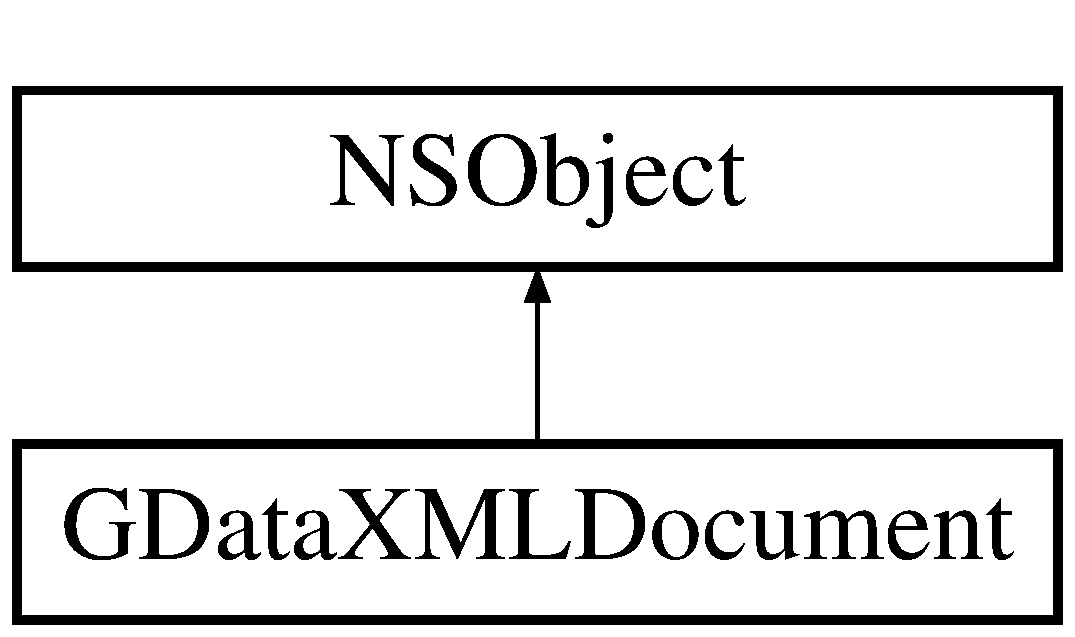
\includegraphics[height=2.000000cm]{interface_g_data_x_m_l_document}
\end{center}
\end{figure}
\subsection*{Instance Methods}
\begin{DoxyCompactItemize}
\item 
\hypertarget{interface_g_data_x_m_l_document_affa6920d0dfcedcd5bc0e21e74af971d}{(id) -\/ {\bfseries init\+With\+X\+M\+L\+String\+:options\+:error\+:}}\label{interface_g_data_x_m_l_document_affa6920d0dfcedcd5bc0e21e74af971d}

\item 
\hypertarget{interface_g_data_x_m_l_document_a5aac20d1849c77ca0904fdd50e65491a}{(id) -\/ {\bfseries init\+With\+Data\+:options\+:error\+:}}\label{interface_g_data_x_m_l_document_a5aac20d1849c77ca0904fdd50e65491a}

\item 
\hypertarget{interface_g_data_x_m_l_document_ab91990967e0e050dfe889f9b67b0d4db}{(id) -\/ {\bfseries init\+With\+Root\+Element\+:}}\label{interface_g_data_x_m_l_document_ab91990967e0e050dfe889f9b67b0d4db}

\item 
\hypertarget{interface_g_data_x_m_l_document_af6e96fd6b07f84044facaf26706f6497}{(\hyperlink{interface_g_data_x_m_l_element}{G\+Data\+X\+M\+L\+Element} $\ast$) -\/ {\bfseries root\+Element}}\label{interface_g_data_x_m_l_document_af6e96fd6b07f84044facaf26706f6497}

\item 
\hypertarget{interface_g_data_x_m_l_document_a984d2f49915376794041612b8c7b0534}{(N\+S\+Data $\ast$) -\/ {\bfseries X\+M\+L\+Data}}\label{interface_g_data_x_m_l_document_a984d2f49915376794041612b8c7b0534}

\item 
\hypertarget{interface_g_data_x_m_l_document_ac43d5fecaa5ca156d4a2202604f63098}{(void) -\/ {\bfseries set\+Version\+:}}\label{interface_g_data_x_m_l_document_ac43d5fecaa5ca156d4a2202604f63098}

\item 
\hypertarget{interface_g_data_x_m_l_document_a4c38b4821cf2fd94e0be91e5f58c47c5}{(void) -\/ {\bfseries set\+Character\+Encoding\+:}}\label{interface_g_data_x_m_l_document_a4c38b4821cf2fd94e0be91e5f58c47c5}

\item 
\hypertarget{interface_g_data_x_m_l_document_a8f72a4eb0c1d63deb9cf99ec44459cc4}{(N\+S\+Array $\ast$) -\/ {\bfseries nodes\+For\+X\+Path\+:namespaces\+:error\+:}}\label{interface_g_data_x_m_l_document_a8f72a4eb0c1d63deb9cf99ec44459cc4}

\item 
\hypertarget{interface_g_data_x_m_l_document_aa354334c070410bde942b706ce83e190}{(N\+S\+Array $\ast$) -\/ {\bfseries nodes\+For\+X\+Path\+:error\+:}}\label{interface_g_data_x_m_l_document_aa354334c070410bde942b706ce83e190}

\item 
\hypertarget{interface_g_data_x_m_l_document_a9bc2a02ba6251d9670127923b43df1a9}{(N\+S\+String $\ast$) -\/ {\bfseries description}}\label{interface_g_data_x_m_l_document_a9bc2a02ba6251d9670127923b43df1a9}

\end{DoxyCompactItemize}
\subsection*{Protected Attributes}
\begin{DoxyCompactItemize}
\item 
\hypertarget{interface_g_data_x_m_l_document_a8ad6e8cee0d74d2b3b28c83099e14e48}{xml\+Doc $\ast$ {\bfseries xml\+Doc\+\_\+}}\label{interface_g_data_x_m_l_document_a8ad6e8cee0d74d2b3b28c83099e14e48}

\end{DoxyCompactItemize}


The documentation for this class was generated from the following files\+:\begin{DoxyCompactItemize}
\item 
Net\+Work/\+X\+M\+L\+Parser/G\+Data\+X\+M\+L\+Node.\+h\item 
Net\+Work/\+X\+M\+L\+Parser/G\+Data\+X\+M\+L\+Node.\+m\end{DoxyCompactItemize}

\hypertarget{category_g_data_x_m_l_document_07_private_methods_08}{\section{G\+Data\+X\+M\+L\+Document(Private\+Methods) Category Reference}
\label{category_g_data_x_m_l_document_07_private_methods_08}\index{G\+Data\+X\+M\+L\+Document(\+Private\+Methods)@{G\+Data\+X\+M\+L\+Document(\+Private\+Methods)}}
}
\subsection*{Instance Methods}
\begin{DoxyCompactItemize}
\item 
\hypertarget{category_g_data_x_m_l_document_07_private_methods_08_a919a4f1c9925f4d6de2c09a92bfd0f35}{(void) -\/ {\bfseries add\+Strings\+Cache\+To\+Doc}}\label{category_g_data_x_m_l_document_07_private_methods_08_a919a4f1c9925f4d6de2c09a92bfd0f35}

\end{DoxyCompactItemize}


The documentation for this category was generated from the following file\+:\begin{DoxyCompactItemize}
\item 
Net\+Work/\+X\+M\+L\+Parser/G\+Data\+X\+M\+L\+Node.\+m\end{DoxyCompactItemize}

\hypertarget{interface_g_data_x_m_l_element}{\section{G\+Data\+X\+M\+L\+Element Class Reference}
\label{interface_g_data_x_m_l_element}\index{G\+Data\+X\+M\+L\+Element@{G\+Data\+X\+M\+L\+Element}}
}
Inheritance diagram for G\+Data\+X\+M\+L\+Element\+:\begin{figure}[H]
\begin{center}
\leavevmode
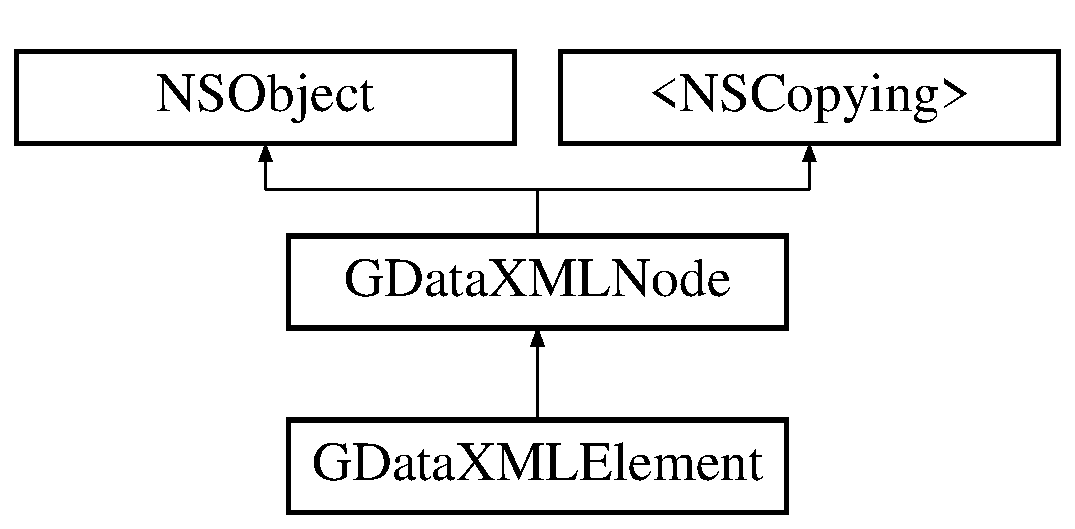
\includegraphics[height=3.000000cm]{interface_g_data_x_m_l_element}
\end{center}
\end{figure}
\subsection*{Instance Methods}
\begin{DoxyCompactItemize}
\item 
\hypertarget{interface_g_data_x_m_l_element_a8020a4dae6ad3175527534d5a793e285}{(id) -\/ {\bfseries init\+With\+X\+M\+L\+String\+:error\+:}}\label{interface_g_data_x_m_l_element_a8020a4dae6ad3175527534d5a793e285}

\item 
\hypertarget{interface_g_data_x_m_l_element_a4c0f13082cdf1115dd51a1199a6c8935}{(N\+S\+Array $\ast$) -\/ {\bfseries namespaces}}\label{interface_g_data_x_m_l_element_a4c0f13082cdf1115dd51a1199a6c8935}

\item 
\hypertarget{interface_g_data_x_m_l_element_af725206ae3ce5c7855a1a2960e82fef7}{(void) -\/ {\bfseries set\+Namespaces\+:}}\label{interface_g_data_x_m_l_element_af725206ae3ce5c7855a1a2960e82fef7}

\item 
\hypertarget{interface_g_data_x_m_l_element_a58f2f9b4dbc512caa8b0a6ac42e907a1}{(void) -\/ {\bfseries add\+Namespace\+:}}\label{interface_g_data_x_m_l_element_a58f2f9b4dbc512caa8b0a6ac42e907a1}

\item 
\hypertarget{interface_g_data_x_m_l_element_a506a65646d411876d1d23b1ce0afa920}{(void) -\/ {\bfseries add\+Child\+:}}\label{interface_g_data_x_m_l_element_a506a65646d411876d1d23b1ce0afa920}

\item 
\hypertarget{interface_g_data_x_m_l_element_a8d9571efd0923ecc365b267fd1c95c8a}{(void) -\/ {\bfseries remove\+Child\+:}}\label{interface_g_data_x_m_l_element_a8d9571efd0923ecc365b267fd1c95c8a}

\item 
\hypertarget{interface_g_data_x_m_l_element_af0724908d7e1c6b831caddcaf7973aaa}{(N\+S\+Array $\ast$) -\/ {\bfseries elements\+For\+Name\+:}}\label{interface_g_data_x_m_l_element_af0724908d7e1c6b831caddcaf7973aaa}

\item 
\hypertarget{interface_g_data_x_m_l_element_af2cb81abe782d2d3396fe9abe3b9f60e}{(N\+S\+Array $\ast$) -\/ {\bfseries elements\+For\+Local\+Name\+:\+U\+R\+I\+:}}\label{interface_g_data_x_m_l_element_af2cb81abe782d2d3396fe9abe3b9f60e}

\item 
\hypertarget{interface_g_data_x_m_l_element_ae6e3e03eff00c20c2953fcbe88d3c4d5}{(N\+S\+Array $\ast$) -\/ {\bfseries attributes}}\label{interface_g_data_x_m_l_element_ae6e3e03eff00c20c2953fcbe88d3c4d5}

\item 
\hypertarget{interface_g_data_x_m_l_element_a0823c7ce613abf40d5913805cbf54a8e}{(\hyperlink{interface_g_data_x_m_l_node}{G\+Data\+X\+M\+L\+Node} $\ast$) -\/ {\bfseries attribute\+For\+Name\+:}}\label{interface_g_data_x_m_l_element_a0823c7ce613abf40d5913805cbf54a8e}

\item 
\hypertarget{interface_g_data_x_m_l_element_aa685fc8bb2453aa2af8543eaa3ac27bc}{(\hyperlink{interface_g_data_x_m_l_node}{G\+Data\+X\+M\+L\+Node} $\ast$) -\/ {\bfseries attribute\+For\+Local\+Name\+:\+U\+R\+I\+:}}\label{interface_g_data_x_m_l_element_aa685fc8bb2453aa2af8543eaa3ac27bc}

\item 
\hypertarget{interface_g_data_x_m_l_element_a51a2307fd7086c0e814fd7b3d5da86bf}{(void) -\/ {\bfseries add\+Attribute\+:}}\label{interface_g_data_x_m_l_element_a51a2307fd7086c0e814fd7b3d5da86bf}

\item 
\hypertarget{interface_g_data_x_m_l_element_ab27be508b932cbe3d0686659069e41b7}{(N\+S\+String $\ast$) -\/ {\bfseries resolve\+Prefix\+For\+Namespace\+U\+R\+I\+:}}\label{interface_g_data_x_m_l_element_ab27be508b932cbe3d0686659069e41b7}

\end{DoxyCompactItemize}
\subsection*{Additional Inherited Members}


The documentation for this class was generated from the following files\+:\begin{DoxyCompactItemize}
\item 
Net\+Work/\+X\+M\+L\+Parser/G\+Data\+X\+M\+L\+Node.\+h\item 
Net\+Work/\+X\+M\+L\+Parser/G\+Data\+X\+M\+L\+Node.\+m\end{DoxyCompactItemize}

\hypertarget{category_g_data_x_m_l_element_07_private_methods_08}{\section{G\+Data\+X\+M\+L\+Element(Private\+Methods) Category Reference}
\label{category_g_data_x_m_l_element_07_private_methods_08}\index{G\+Data\+X\+M\+L\+Element(\+Private\+Methods)@{G\+Data\+X\+M\+L\+Element(\+Private\+Methods)}}
}
\subsection*{Class Methods}
\begin{DoxyCompactItemize}
\item 
\hypertarget{category_g_data_x_m_l_element_07_private_methods_08_a5f56aa547c9ba1abdc3d68e050a9b4e3}{(void) + {\bfseries fix\+Up\+Namespaces\+For\+Node\+:grafting\+To\+Tree\+Node\+:}}\label{category_g_data_x_m_l_element_07_private_methods_08_a5f56aa547c9ba1abdc3d68e050a9b4e3}

\end{DoxyCompactItemize}


The documentation for this category was generated from the following file\+:\begin{DoxyCompactItemize}
\item 
Net\+Work/\+X\+M\+L\+Parser/G\+Data\+X\+M\+L\+Node.\+m\end{DoxyCompactItemize}

\hypertarget{interface_g_data_x_m_l_node}{\section{G\+Data\+X\+M\+L\+Node Class Reference}
\label{interface_g_data_x_m_l_node}\index{G\+Data\+X\+M\+L\+Node@{G\+Data\+X\+M\+L\+Node}}
}
Inheritance diagram for G\+Data\+X\+M\+L\+Node\+:\begin{figure}[H]
\begin{center}
\leavevmode
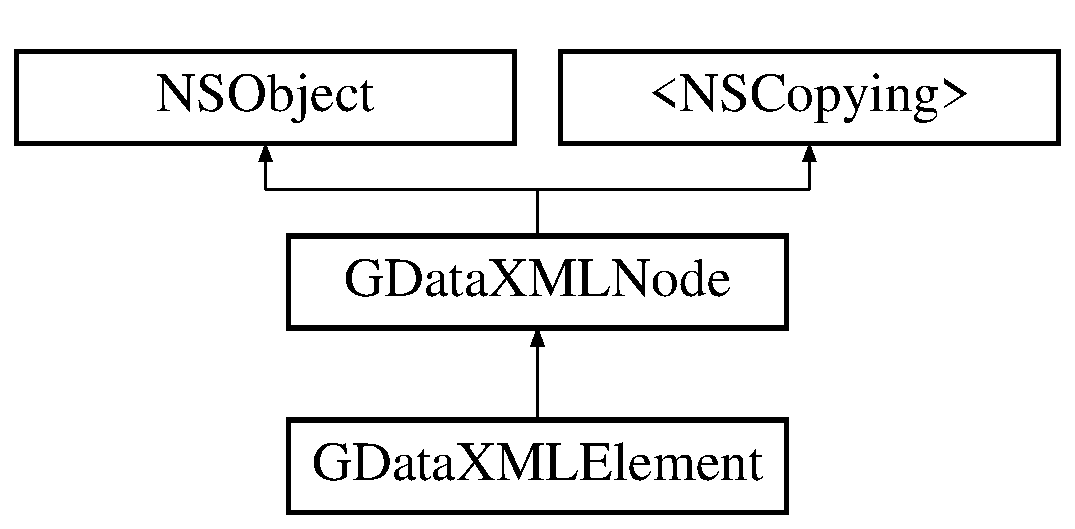
\includegraphics[height=3.000000cm]{interface_g_data_x_m_l_node}
\end{center}
\end{figure}
\subsection*{Instance Methods}
\begin{DoxyCompactItemize}
\item 
\hypertarget{interface_g_data_x_m_l_node_ad6cef8a7c9c6714b8ea42e2620f86866}{(N\+S\+String $\ast$) -\/ {\bfseries string\+Value}}\label{interface_g_data_x_m_l_node_ad6cef8a7c9c6714b8ea42e2620f86866}

\item 
\hypertarget{interface_g_data_x_m_l_node_ab3b73dcb1ac9607325552747a3055a1e}{(void) -\/ {\bfseries set\+String\+Value\+:}}\label{interface_g_data_x_m_l_node_ab3b73dcb1ac9607325552747a3055a1e}

\item 
\hypertarget{interface_g_data_x_m_l_node_a8c1ecef5a1827105f8cdb435fe330dda}{(N\+S\+U\+Integer) -\/ {\bfseries child\+Count}}\label{interface_g_data_x_m_l_node_a8c1ecef5a1827105f8cdb435fe330dda}

\item 
\hypertarget{interface_g_data_x_m_l_node_a5d78f07c8cd059176801973bf6883452}{(N\+S\+Array $\ast$) -\/ {\bfseries children}}\label{interface_g_data_x_m_l_node_a5d78f07c8cd059176801973bf6883452}

\item 
\hypertarget{interface_g_data_x_m_l_node_acabc5e624c3bbc27ba75c443d48b9795}{(\hyperlink{interface_g_data_x_m_l_node}{G\+Data\+X\+M\+L\+Node} $\ast$) -\/ {\bfseries child\+At\+Index\+:}}\label{interface_g_data_x_m_l_node_acabc5e624c3bbc27ba75c443d48b9795}

\item 
\hypertarget{interface_g_data_x_m_l_node_a503afc6b19e456b831f6b45ae184336c}{(N\+S\+String $\ast$) -\/ {\bfseries local\+Name}}\label{interface_g_data_x_m_l_node_a503afc6b19e456b831f6b45ae184336c}

\item 
\hypertarget{interface_g_data_x_m_l_node_a4dcfed52258221c7387f1482d7ee8488}{(N\+S\+String $\ast$) -\/ {\bfseries name}}\label{interface_g_data_x_m_l_node_a4dcfed52258221c7387f1482d7ee8488}

\item 
\hypertarget{interface_g_data_x_m_l_node_ad243c0aec788b95cb5fa8b6a89707c10}{(N\+S\+String $\ast$) -\/ {\bfseries prefix}}\label{interface_g_data_x_m_l_node_ad243c0aec788b95cb5fa8b6a89707c10}

\item 
\hypertarget{interface_g_data_x_m_l_node_a9d34ab47a4b5e1b3c67b26b07e9956a1}{(N\+S\+String $\ast$) -\/ {\bfseries U\+R\+I}}\label{interface_g_data_x_m_l_node_a9d34ab47a4b5e1b3c67b26b07e9956a1}

\item 
\hypertarget{interface_g_data_x_m_l_node_a5e033ccdae3236c8875e1c6feb44c949}{(G\+Data\+X\+M\+L\+Node\+Kind) -\/ {\bfseries kind}}\label{interface_g_data_x_m_l_node_a5e033ccdae3236c8875e1c6feb44c949}

\item 
\hypertarget{interface_g_data_x_m_l_node_a958c434d973db58ada939d7276977812}{(N\+S\+String $\ast$) -\/ {\bfseries X\+M\+L\+String}}\label{interface_g_data_x_m_l_node_a958c434d973db58ada939d7276977812}

\item 
\hypertarget{interface_g_data_x_m_l_node_a93c2784d84fc245d99cf2943fc41c19c}{(N\+S\+Array $\ast$) -\/ {\bfseries nodes\+For\+X\+Path\+:namespaces\+:error\+:}}\label{interface_g_data_x_m_l_node_a93c2784d84fc245d99cf2943fc41c19c}

\item 
\hypertarget{interface_g_data_x_m_l_node_a48f3179efdba9b7e017aa32e7118907b}{(N\+S\+Array $\ast$) -\/ {\bfseries nodes\+For\+X\+Path\+:error\+:}}\label{interface_g_data_x_m_l_node_a48f3179efdba9b7e017aa32e7118907b}

\item 
\hypertarget{interface_g_data_x_m_l_node_a775ef8bdbcb26003bfd326930f028d44}{(xml\+Node\+Ptr) -\/ {\bfseries X\+M\+L\+Node}}\label{interface_g_data_x_m_l_node_a775ef8bdbcb26003bfd326930f028d44}

\item 
\hypertarget{interface_g_data_x_m_l_node_a71cb5af09b5c6737c452f2e09bcdec36}{(void) -\/ {\bfseries release\+Cached\+Values}}\label{interface_g_data_x_m_l_node_a71cb5af09b5c6737c452f2e09bcdec36}

\end{DoxyCompactItemize}
\subsection*{Class Methods}
\begin{DoxyCompactItemize}
\item 
\hypertarget{interface_g_data_x_m_l_node_ad7e4405c6195d993a5633faa1899c8a0}{(\hyperlink{interface_g_data_x_m_l_element}{G\+Data\+X\+M\+L\+Element} $\ast$) + {\bfseries element\+With\+Name\+:}}\label{interface_g_data_x_m_l_node_ad7e4405c6195d993a5633faa1899c8a0}

\item 
\hypertarget{interface_g_data_x_m_l_node_ad8afb69afa7b083627e8a6db5eba45f7}{(\hyperlink{interface_g_data_x_m_l_element}{G\+Data\+X\+M\+L\+Element} $\ast$) + {\bfseries element\+With\+Name\+:string\+Value\+:}}\label{interface_g_data_x_m_l_node_ad8afb69afa7b083627e8a6db5eba45f7}

\item 
\hypertarget{interface_g_data_x_m_l_node_ae1241290bcd76d378ba9a5eb0612b6c4}{(\hyperlink{interface_g_data_x_m_l_element}{G\+Data\+X\+M\+L\+Element} $\ast$) + {\bfseries element\+With\+Name\+:\+U\+R\+I\+:}}\label{interface_g_data_x_m_l_node_ae1241290bcd76d378ba9a5eb0612b6c4}

\item 
\hypertarget{interface_g_data_x_m_l_node_abd922c9940730a4f78c906c2392123df}{(id) + {\bfseries attribute\+With\+Name\+:string\+Value\+:}}\label{interface_g_data_x_m_l_node_abd922c9940730a4f78c906c2392123df}

\item 
\hypertarget{interface_g_data_x_m_l_node_a82060803e76687ce902f09c96f654ab2}{(id) + {\bfseries attribute\+With\+Name\+:\+U\+R\+I\+:string\+Value\+:}}\label{interface_g_data_x_m_l_node_a82060803e76687ce902f09c96f654ab2}

\item 
\hypertarget{interface_g_data_x_m_l_node_a59cd9e673bcf2be9ed19ebbabc68ad26}{(id) + {\bfseries namespace\+With\+Name\+:string\+Value\+:}}\label{interface_g_data_x_m_l_node_a59cd9e673bcf2be9ed19ebbabc68ad26}

\item 
\hypertarget{interface_g_data_x_m_l_node_a13761fd3b75c6f465800e2d4ae45db84}{(id) + {\bfseries text\+With\+String\+Value\+:}}\label{interface_g_data_x_m_l_node_a13761fd3b75c6f465800e2d4ae45db84}

\item 
\hypertarget{interface_g_data_x_m_l_node_abaa7cb3204ca104a89895f895728b942}{(N\+S\+String $\ast$) + {\bfseries local\+Name\+For\+Name\+:}}\label{interface_g_data_x_m_l_node_abaa7cb3204ca104a89895f895728b942}

\item 
\hypertarget{interface_g_data_x_m_l_node_ad6038ded1bfe166d7c87718dde7a466f}{(N\+S\+String $\ast$) + {\bfseries prefix\+For\+Name\+:}}\label{interface_g_data_x_m_l_node_ad6038ded1bfe166d7c87718dde7a466f}

\end{DoxyCompactItemize}
\subsection*{Protected Attributes}
\begin{DoxyCompactItemize}
\item 
\hypertarget{interface_g_data_x_m_l_node_acfd13d67dcb0ed8011df204c36c88d6f}{xml\+Node\+Ptr {\bfseries xml\+Node\+\_\+}}\label{interface_g_data_x_m_l_node_acfd13d67dcb0ed8011df204c36c88d6f}

\item 
\hypertarget{interface_g_data_x_m_l_node_af6ca9b5845f17e614acc517388e1bfd5}{B\+O\+O\+L {\bfseries should\+Free\+X\+M\+L\+Node\+\_\+}}\label{interface_g_data_x_m_l_node_af6ca9b5845f17e614acc517388e1bfd5}

\item 
\hypertarget{interface_g_data_x_m_l_node_abf237c0ffe4081e69064e6ca858b23c6}{N\+S\+String $\ast$ {\bfseries cached\+Name\+\_\+}}\label{interface_g_data_x_m_l_node_abf237c0ffe4081e69064e6ca858b23c6}

\item 
\hypertarget{interface_g_data_x_m_l_node_a4bf9ed070da05d56e7af4481d7e85c3b}{N\+S\+Array $\ast$ {\bfseries cached\+Children\+\_\+}}\label{interface_g_data_x_m_l_node_a4bf9ed070da05d56e7af4481d7e85c3b}

\item 
\hypertarget{interface_g_data_x_m_l_node_a5681557d48aaa1ed6ba6a5d6488bb6a5}{N\+S\+Array $\ast$ {\bfseries cached\+Attributes\+\_\+}}\label{interface_g_data_x_m_l_node_a5681557d48aaa1ed6ba6a5d6488bb6a5}

\end{DoxyCompactItemize}


The documentation for this class was generated from the following files\+:\begin{DoxyCompactItemize}
\item 
Net\+Work/\+X\+M\+L\+Parser/G\+Data\+X\+M\+L\+Node.\+h\item 
Net\+Work/\+X\+M\+L\+Parser/G\+Data\+X\+M\+L\+Node.\+m\end{DoxyCompactItemize}

\hypertarget{category_g_data_x_m_l_node_07_private_methods_08}{\section{G\+Data\+X\+M\+L\+Node(Private\+Methods) Category Reference}
\label{category_g_data_x_m_l_node_07_private_methods_08}\index{G\+Data\+X\+M\+L\+Node(\+Private\+Methods)@{G\+Data\+X\+M\+L\+Node(\+Private\+Methods)}}
}
\subsection*{Instance Methods}
\begin{DoxyCompactItemize}
\item 
\hypertarget{category_g_data_x_m_l_node_07_private_methods_08_afe892d98b556fbab1381efd9fcde6819}{(id) -\/ {\bfseries init\+Consuming\+X\+M\+L\+Node\+:}}\label{category_g_data_x_m_l_node_07_private_methods_08_afe892d98b556fbab1381efd9fcde6819}

\item 
\hypertarget{category_g_data_x_m_l_node_07_private_methods_08_ac32928fffb81e4e96957c82e759fd192}{(id) -\/ {\bfseries init\+Borrowing\+X\+M\+L\+Node\+:}}\label{category_g_data_x_m_l_node_07_private_methods_08_ac32928fffb81e4e96957c82e759fd192}

\item 
\hypertarget{category_g_data_x_m_l_node_07_private_methods_08_a472c0a766d820c7774f5c587e32db00d}{(xml\+Node\+Ptr) -\/ {\bfseries X\+M\+L\+Node}}\label{category_g_data_x_m_l_node_07_private_methods_08_a472c0a766d820c7774f5c587e32db00d}

\item 
\hypertarget{category_g_data_x_m_l_node_07_private_methods_08_af9ab19e292ae4d18c6302f97f6e284f8}{(xml\+Node\+Ptr) -\/ {\bfseries X\+M\+L\+Node\+Copy}}\label{category_g_data_x_m_l_node_07_private_methods_08_af9ab19e292ae4d18c6302f97f6e284f8}

\item 
\hypertarget{category_g_data_x_m_l_node_07_private_methods_08_adbb4de0b3d2e31e5016413f28df8ab23}{(\hyperlink{interface_g_data_x_m_l_node}{G\+Data\+X\+M\+L\+Node} $\ast$) -\/ {\bfseries attribute\+For\+X\+M\+L\+Node\+:}}\label{category_g_data_x_m_l_node_07_private_methods_08_adbb4de0b3d2e31e5016413f28df8ab23}

\item 
\hypertarget{category_g_data_x_m_l_node_07_private_methods_08_aab0df9eaa8a836f244fc035ceada7901}{(N\+S\+String $\ast$) -\/ {\bfseries string\+From\+X\+M\+L\+String\+:}}\label{category_g_data_x_m_l_node_07_private_methods_08_aab0df9eaa8a836f244fc035ceada7901}

\item 
\hypertarget{category_g_data_x_m_l_node_07_private_methods_08_a7d6b77d179a4a83b5cfe0c173baf1c3c}{(B\+O\+O\+L) -\/ {\bfseries should\+Free\+X\+M\+L\+Node}}\label{category_g_data_x_m_l_node_07_private_methods_08_a7d6b77d179a4a83b5cfe0c173baf1c3c}

\item 
\hypertarget{category_g_data_x_m_l_node_07_private_methods_08_a0faeb14e174431b0f7b6e90e5bb14e21}{(void) -\/ {\bfseries set\+Should\+Free\+X\+M\+L\+Node\+:}}\label{category_g_data_x_m_l_node_07_private_methods_08_a0faeb14e174431b0f7b6e90e5bb14e21}

\end{DoxyCompactItemize}
\subsection*{Class Methods}
\begin{DoxyCompactItemize}
\item 
\hypertarget{category_g_data_x_m_l_node_07_private_methods_08_afa291e610c39be001971719e6eb37996}{(id) + {\bfseries node\+Consuming\+X\+M\+L\+Node\+:}}\label{category_g_data_x_m_l_node_07_private_methods_08_afa291e610c39be001971719e6eb37996}

\item 
\hypertarget{category_g_data_x_m_l_node_07_private_methods_08_a0b67aacd8d9351afa5d159b3971b932f}{(id) + {\bfseries node\+Borrowing\+X\+M\+L\+Node\+:}}\label{category_g_data_x_m_l_node_07_private_methods_08_a0b67aacd8d9351afa5d159b3971b932f}

\end{DoxyCompactItemize}


The documentation for this category was generated from the following file\+:\begin{DoxyCompactItemize}
\item 
Net\+Work/\+X\+M\+L\+Parser/G\+Data\+X\+M\+L\+Node.\+m\end{DoxyCompactItemize}

\hypertarget{interface_j_k_array}{\section{J\+K\+Array Class Reference}
\label{interface_j_k_array}\index{J\+K\+Array@{J\+K\+Array}}
}
Inheritance diagram for J\+K\+Array\+:\begin{figure}[H]
\begin{center}
\leavevmode
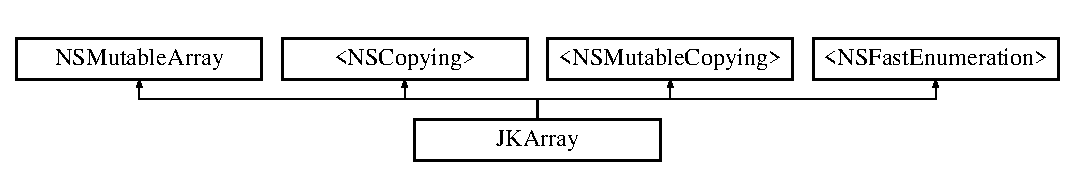
\includegraphics[height=1.931034cm]{interface_j_k_array}
\end{center}
\end{figure}
\subsection*{Protected Attributes}
\begin{DoxyCompactItemize}
\item 
\hypertarget{interface_j_k_array_a26bec99d019d3ec883d849986e2c3ef9}{id $\ast$ {\bfseries objects}}\label{interface_j_k_array_a26bec99d019d3ec883d849986e2c3ef9}

\item 
\hypertarget{interface_j_k_array_a903336bb8564dd3b732b4a0aab7dfb48}{N\+S\+U\+Integer {\bfseries count}}\label{interface_j_k_array_a903336bb8564dd3b732b4a0aab7dfb48}

\item 
\hypertarget{interface_j_k_array_a74b14ae533a3004ac5eef33d06c59470}{N\+S\+U\+Integer {\bfseries capacity}}\label{interface_j_k_array_a74b14ae533a3004ac5eef33d06c59470}

\item 
\hypertarget{interface_j_k_array_af5ad2eeccbca0b4203feb674a975aaf4}{N\+S\+U\+Integer {\bfseries mutations}}\label{interface_j_k_array_af5ad2eeccbca0b4203feb674a975aaf4}

\end{DoxyCompactItemize}


The documentation for this class was generated from the following file\+:\begin{DoxyCompactItemize}
\item 
J\+S\+O\+N\+Kit/J\+S\+O\+N\+Kit.\+m\end{DoxyCompactItemize}

\hypertarget{struct_j_k_buffer}{\section{J\+K\+Buffer Struct Reference}
\label{struct_j_k_buffer}\index{J\+K\+Buffer@{J\+K\+Buffer}}
}
\subsection*{Protected Attributes}
\begin{DoxyCompactItemize}
\item 
\hypertarget{struct_j_k_buffer_a82b694da8e8cc43e460b548581b1dc03}{\hyperlink{struct_j_k_ptr_range}{J\+K\+Ptr\+Range} {\bfseries bytes}}\label{struct_j_k_buffer_a82b694da8e8cc43e460b548581b1dc03}

\end{DoxyCompactItemize}


The documentation for this struct was generated from the following file\+:\begin{DoxyCompactItemize}
\item 
J\+S\+O\+N\+Kit/J\+S\+O\+N\+Kit.\+m\end{DoxyCompactItemize}

\hypertarget{struct_j_k_const_buffer}{\section{J\+K\+Const\+Buffer Struct Reference}
\label{struct_j_k_const_buffer}\index{J\+K\+Const\+Buffer@{J\+K\+Const\+Buffer}}
}
\subsection*{Protected Attributes}
\begin{DoxyCompactItemize}
\item 
\hypertarget{struct_j_k_const_buffer_ac9eed12dee7b6758b0672a86ba4d1e73}{\hyperlink{struct_j_k_const_ptr_range}{J\+K\+Const\+Ptr\+Range} {\bfseries bytes}}\label{struct_j_k_const_buffer_ac9eed12dee7b6758b0672a86ba4d1e73}

\end{DoxyCompactItemize}


The documentation for this struct was generated from the following file\+:\begin{DoxyCompactItemize}
\item 
J\+S\+O\+N\+Kit/J\+S\+O\+N\+Kit.\+m\end{DoxyCompactItemize}

\hypertarget{struct_j_k_const_ptr_range}{\section{J\+K\+Const\+Ptr\+Range Struct Reference}
\label{struct_j_k_const_ptr_range}\index{J\+K\+Const\+Ptr\+Range@{J\+K\+Const\+Ptr\+Range}}
}
\subsection*{Protected Attributes}
\begin{DoxyCompactItemize}
\item 
\hypertarget{struct_j_k_const_ptr_range_afa2519e22b4232f1e2e01f23b5c3df4f}{const unsigned char $\ast$ {\bfseries ptr}}\label{struct_j_k_const_ptr_range_afa2519e22b4232f1e2e01f23b5c3df4f}

\item 
\hypertarget{struct_j_k_const_ptr_range_a71e6d672adc0a4ab55448c2bb585d582}{size\+\_\+t {\bfseries length}}\label{struct_j_k_const_ptr_range_a71e6d672adc0a4ab55448c2bb585d582}

\end{DoxyCompactItemize}


The documentation for this struct was generated from the following file\+:\begin{DoxyCompactItemize}
\item 
J\+S\+O\+N\+Kit/J\+S\+O\+N\+Kit.\+m\end{DoxyCompactItemize}

\hypertarget{interface_j_k_dictionary}{\section{J\+K\+Dictionary Class Reference}
\label{interface_j_k_dictionary}\index{J\+K\+Dictionary@{J\+K\+Dictionary}}
}
Inheritance diagram for J\+K\+Dictionary\+:\begin{figure}[H]
\begin{center}
\leavevmode
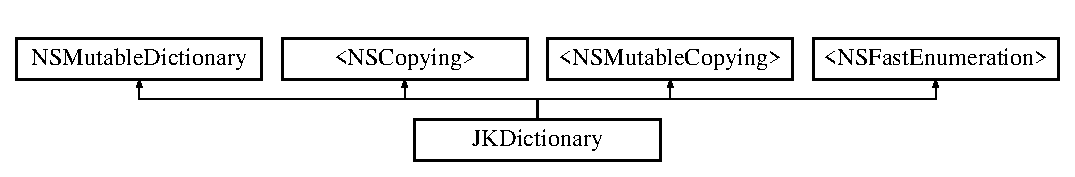
\includegraphics[height=1.931034cm]{interface_j_k_dictionary}
\end{center}
\end{figure}
\subsection*{Protected Attributes}
\begin{DoxyCompactItemize}
\item 
\hypertarget{interface_j_k_dictionary_af9a788a17e658c6f1b66a24fd9b1b42a}{N\+S\+U\+Integer {\bfseries count}}\label{interface_j_k_dictionary_af9a788a17e658c6f1b66a24fd9b1b42a}

\item 
\hypertarget{interface_j_k_dictionary_a0573bbe8650a3d8b075b8f06fd9fe3c6}{N\+S\+U\+Integer {\bfseries capacity}}\label{interface_j_k_dictionary_a0573bbe8650a3d8b075b8f06fd9fe3c6}

\item 
\hypertarget{interface_j_k_dictionary_ac7f772c0ef0a376a4fe48aca3496ccb3}{N\+S\+U\+Integer {\bfseries mutations}}\label{interface_j_k_dictionary_ac7f772c0ef0a376a4fe48aca3496ccb3}

\item 
\hypertarget{interface_j_k_dictionary_ad329317a4a2c0076e67efc69cfc45830}{\hyperlink{struct_j_k_hash_table_entry}{J\+K\+Hash\+Table\+Entry} $\ast$ {\bfseries entry}}\label{interface_j_k_dictionary_ad329317a4a2c0076e67efc69cfc45830}

\end{DoxyCompactItemize}


The documentation for this class was generated from the following file\+:\begin{DoxyCompactItemize}
\item 
J\+S\+O\+N\+Kit/J\+S\+O\+N\+Kit.\+m\end{DoxyCompactItemize}

\hypertarget{interface_j_k_dictionary_enumerator}{\section{J\+K\+Dictionary\+Enumerator Class Reference}
\label{interface_j_k_dictionary_enumerator}\index{J\+K\+Dictionary\+Enumerator@{J\+K\+Dictionary\+Enumerator}}
}
Inheritance diagram for J\+K\+Dictionary\+Enumerator\+:\begin{figure}[H]
\begin{center}
\leavevmode
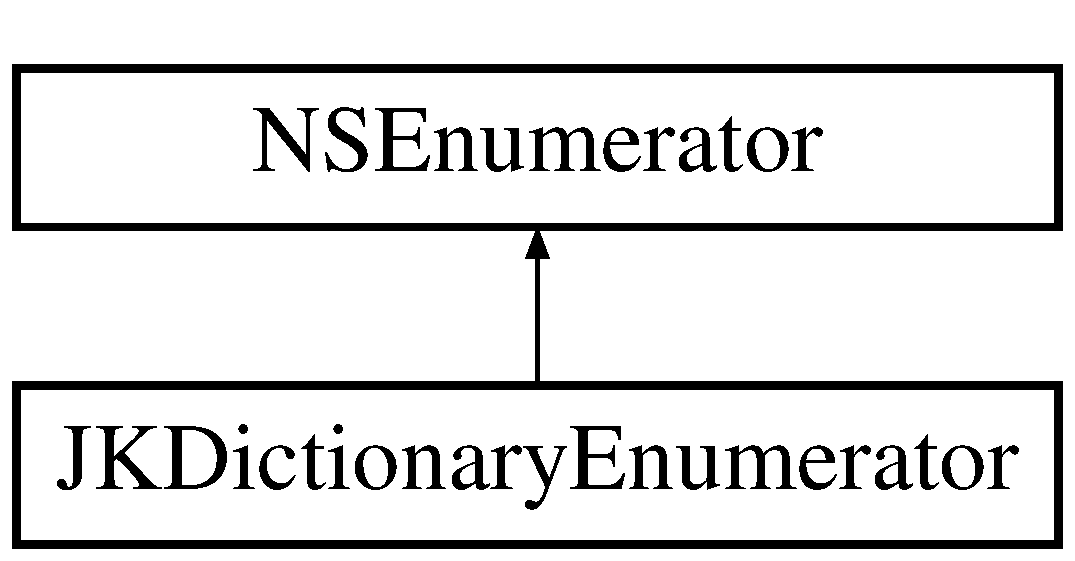
\includegraphics[height=2.000000cm]{interface_j_k_dictionary_enumerator}
\end{center}
\end{figure}
\subsection*{Instance Methods}
\begin{DoxyCompactItemize}
\item 
\hypertarget{interface_j_k_dictionary_enumerator_a5085cc23ae119b8cdf4328f8333e6ae7}{(id) -\/ {\bfseries init\+With\+J\+K\+Dictionary\+:}}\label{interface_j_k_dictionary_enumerator_a5085cc23ae119b8cdf4328f8333e6ae7}

\item 
\hypertarget{interface_j_k_dictionary_enumerator_aeacc476cb120593fb2b140e019427c97}{(N\+S\+Array $\ast$) -\/ {\bfseries all\+Objects}}\label{interface_j_k_dictionary_enumerator_aeacc476cb120593fb2b140e019427c97}

\item 
\hypertarget{interface_j_k_dictionary_enumerator_ae72411e7e1dda3b91950ddcd210bb7cf}{(id) -\/ {\bfseries next\+Object}}\label{interface_j_k_dictionary_enumerator_ae72411e7e1dda3b91950ddcd210bb7cf}

\end{DoxyCompactItemize}
\subsection*{Protected Attributes}
\begin{DoxyCompactItemize}
\item 
\hypertarget{interface_j_k_dictionary_enumerator_a58e8ed040636b59b6c9eaeb0dc6c89f2}{id {\bfseries collection}}\label{interface_j_k_dictionary_enumerator_a58e8ed040636b59b6c9eaeb0dc6c89f2}

\item 
\hypertarget{interface_j_k_dictionary_enumerator_add4b08edabce81c31438ec3c16cd37d8}{N\+S\+U\+Integer {\bfseries next\+Object}}\label{interface_j_k_dictionary_enumerator_add4b08edabce81c31438ec3c16cd37d8}

\end{DoxyCompactItemize}


The documentation for this class was generated from the following file\+:\begin{DoxyCompactItemize}
\item 
J\+S\+O\+N\+Kit/J\+S\+O\+N\+Kit.\+m\end{DoxyCompactItemize}

\hypertarget{struct_j_k_encode_cache}{\section{J\+K\+Encode\+Cache Struct Reference}
\label{struct_j_k_encode_cache}\index{J\+K\+Encode\+Cache@{J\+K\+Encode\+Cache}}
}
\subsection*{Protected Attributes}
\begin{DoxyCompactItemize}
\item 
\hypertarget{struct_j_k_encode_cache_a92d31ee910f818f9d319db5f6e1a17f0}{id {\bfseries object}}\label{struct_j_k_encode_cache_a92d31ee910f818f9d319db5f6e1a17f0}

\item 
\hypertarget{struct_j_k_encode_cache_a7651dd8a8d77c384a286f0a6432a6a30}{size\+\_\+t {\bfseries offset}}\label{struct_j_k_encode_cache_a7651dd8a8d77c384a286f0a6432a6a30}

\item 
\hypertarget{struct_j_k_encode_cache_a8d75c9aafedd78bd41f58a7cae621a5a}{size\+\_\+t {\bfseries length}}\label{struct_j_k_encode_cache_a8d75c9aafedd78bd41f58a7cae621a5a}

\end{DoxyCompactItemize}


The documentation for this struct was generated from the following file\+:\begin{DoxyCompactItemize}
\item 
J\+S\+O\+N\+Kit/J\+S\+O\+N\+Kit.\+m\end{DoxyCompactItemize}

\hypertarget{struct_j_k_encode_state}{\section{J\+K\+Encode\+State Struct Reference}
\label{struct_j_k_encode_state}\index{J\+K\+Encode\+State@{J\+K\+Encode\+State}}
}
\subsection*{Protected Attributes}
\begin{DoxyCompactItemize}
\item 
\hypertarget{struct_j_k_encode_state_a1b0aea46e1e8d3c3c1a10c717b62e594}{\hyperlink{struct_j_k_managed_buffer}{J\+K\+Managed\+Buffer} {\bfseries utf8\+Conversion\+Buffer}}\label{struct_j_k_encode_state_a1b0aea46e1e8d3c3c1a10c717b62e594}

\item 
\hypertarget{struct_j_k_encode_state_a75a3a02fa81cbff32df3dd039bb1516e}{\hyperlink{struct_j_k_managed_buffer}{J\+K\+Managed\+Buffer} {\bfseries string\+Buffer}}\label{struct_j_k_encode_state_a75a3a02fa81cbff32df3dd039bb1516e}

\item 
\hypertarget{struct_j_k_encode_state_a74e949afd40d30d6bf3f90283fce0ffb}{size\+\_\+t {\bfseries at\+Index}}\label{struct_j_k_encode_state_a74e949afd40d30d6bf3f90283fce0ffb}

\item 
\hypertarget{struct_j_k_encode_state_afa5f38579b9be63a088d6e7633280998}{\hyperlink{struct_j_k_fast_class_lookup}{J\+K\+Fast\+Class\+Lookup} {\bfseries fast\+Class\+Lookup}}\label{struct_j_k_encode_state_afa5f38579b9be63a088d6e7633280998}

\item 
\hypertarget{struct_j_k_encode_state_a0ef51a24eff707dcbf33ae7247214d21}{\hyperlink{struct_j_k_encode_cache}{J\+K\+Encode\+Cache} {\bfseries cache} \mbox{[}J\+K\+\_\+\+E\+N\+C\+O\+D\+E\+\_\+\+C\+A\+C\+H\+E\+\_\+\+S\+L\+O\+T\+S\mbox{]}}\label{struct_j_k_encode_state_a0ef51a24eff707dcbf33ae7247214d21}

\item 
\hypertarget{struct_j_k_encode_state_ac12503e3307839b27c7d91e1fcb503c8}{J\+K\+Serialize\+Option\+Flags {\bfseries serialize\+Option\+Flags}}\label{struct_j_k_encode_state_ac12503e3307839b27c7d91e1fcb503c8}

\item 
\hypertarget{struct_j_k_encode_state_a8f92a733bcd0a24441b86fdf44746a2b}{J\+K\+Encode\+Option\+Type {\bfseries encode\+Option}}\label{struct_j_k_encode_state_a8f92a733bcd0a24441b86fdf44746a2b}

\item 
\hypertarget{struct_j_k_encode_state_a0f95ac1d47e8408d4108e12d226b6fc2}{size\+\_\+t {\bfseries depth}}\label{struct_j_k_encode_state_a0f95ac1d47e8408d4108e12d226b6fc2}

\item 
\hypertarget{struct_j_k_encode_state_a06a37dda06467b599ec7b24093b4982f}{N\+S\+Error $\ast$ {\bfseries error}}\label{struct_j_k_encode_state_a06a37dda06467b599ec7b24093b4982f}

\item 
\hypertarget{struct_j_k_encode_state_a15a9d6710ae0bd0851fcc7d9756768a6}{id {\bfseries class\+Formatter\+Delegate}}\label{struct_j_k_encode_state_a15a9d6710ae0bd0851fcc7d9756768a6}

\item 
\hypertarget{struct_j_k_encode_state_ad29de3691eba8128cd70cc5f362f60d0}{S\+E\+L {\bfseries class\+Formatter\+Selector}}\label{struct_j_k_encode_state_ad29de3691eba8128cd70cc5f362f60d0}

\item 
\hypertarget{struct_j_k_encode_state_a8f58e19530ef145df0ecf1ac35865d2e}{J\+K\+Class\+Formatter\+I\+M\+P {\bfseries class\+Formatter\+I\+M\+P}}\label{struct_j_k_encode_state_a8f58e19530ef145df0ecf1ac35865d2e}

\end{DoxyCompactItemize}


The documentation for this struct was generated from the following file\+:\begin{DoxyCompactItemize}
\item 
J\+S\+O\+N\+Kit/J\+S\+O\+N\+Kit.\+m\end{DoxyCompactItemize}

\hypertarget{struct_j_k_fast_class_lookup}{\section{J\+K\+Fast\+Class\+Lookup Struct Reference}
\label{struct_j_k_fast_class_lookup}\index{J\+K\+Fast\+Class\+Lookup@{J\+K\+Fast\+Class\+Lookup}}
}
\subsection*{Protected Attributes}
\begin{DoxyCompactItemize}
\item 
\hypertarget{struct_j_k_fast_class_lookup_acd04a4b7e019d6a55790817b854128a2}{void $\ast$ {\bfseries string\+Class}}\label{struct_j_k_fast_class_lookup_acd04a4b7e019d6a55790817b854128a2}

\item 
\hypertarget{struct_j_k_fast_class_lookup_a603079acbc76d7743d135768f77baa85}{void $\ast$ {\bfseries number\+Class}}\label{struct_j_k_fast_class_lookup_a603079acbc76d7743d135768f77baa85}

\item 
\hypertarget{struct_j_k_fast_class_lookup_ab0f7be4ff84fd61097b479e03cb6de94}{void $\ast$ {\bfseries array\+Class}}\label{struct_j_k_fast_class_lookup_ab0f7be4ff84fd61097b479e03cb6de94}

\item 
\hypertarget{struct_j_k_fast_class_lookup_a52147c32a09cabb2ffa9ff7ac1a27e5b}{void $\ast$ {\bfseries dictionary\+Class}}\label{struct_j_k_fast_class_lookup_a52147c32a09cabb2ffa9ff7ac1a27e5b}

\item 
\hypertarget{struct_j_k_fast_class_lookup_a8399859e5563a816499b6d2ffdfb55ca}{void $\ast$ {\bfseries null\+Class}}\label{struct_j_k_fast_class_lookup_a8399859e5563a816499b6d2ffdfb55ca}

\end{DoxyCompactItemize}


The documentation for this struct was generated from the following file\+:\begin{DoxyCompactItemize}
\item 
J\+S\+O\+N\+Kit/J\+S\+O\+N\+Kit.\+m\end{DoxyCompactItemize}

\hypertarget{struct_j_k_hash_table_entry}{\section{J\+K\+Hash\+Table\+Entry Struct Reference}
\label{struct_j_k_hash_table_entry}\index{J\+K\+Hash\+Table\+Entry@{J\+K\+Hash\+Table\+Entry}}
}
\subsection*{Protected Attributes}
\begin{DoxyCompactItemize}
\item 
\hypertarget{struct_j_k_hash_table_entry_a3627d1eea6b9d771b73d460d110a125a}{N\+S\+U\+Integer {\bfseries key\+Hash}}\label{struct_j_k_hash_table_entry_a3627d1eea6b9d771b73d460d110a125a}

\item 
\hypertarget{struct_j_k_hash_table_entry_a14459841f0c97cce172556d8338234bd}{id {\bfseries key}}\label{struct_j_k_hash_table_entry_a14459841f0c97cce172556d8338234bd}

\item 
\hypertarget{struct_j_k_hash_table_entry_a47f523fa961c85cbb5df375b802b8316}{id {\bfseries object}}\label{struct_j_k_hash_table_entry_a47f523fa961c85cbb5df375b802b8316}

\end{DoxyCompactItemize}


The documentation for this struct was generated from the following file\+:\begin{DoxyCompactItemize}
\item 
J\+S\+O\+N\+Kit/J\+S\+O\+N\+Kit.\+m\end{DoxyCompactItemize}

\hypertarget{struct_j_k_managed_buffer}{\section{J\+K\+Managed\+Buffer Struct Reference}
\label{struct_j_k_managed_buffer}\index{J\+K\+Managed\+Buffer@{J\+K\+Managed\+Buffer}}
}
\subsection*{Protected Attributes}
\begin{DoxyCompactItemize}
\item 
\hypertarget{struct_j_k_managed_buffer_a57af888785f75f4282fe68215655e146}{\hyperlink{struct_j_k_ptr_range}{J\+K\+Ptr\+Range} {\bfseries bytes}}\label{struct_j_k_managed_buffer_a57af888785f75f4282fe68215655e146}

\item 
\hypertarget{struct_j_k_managed_buffer_a38a499c041d11c99bc175f53c3700c5a}{J\+K\+Managed\+Buffer\+Flags {\bfseries flags}}\label{struct_j_k_managed_buffer_a38a499c041d11c99bc175f53c3700c5a}

\item 
\hypertarget{struct_j_k_managed_buffer_ad45389f30f38ea703e116ba4f7496fc2}{size\+\_\+t {\bfseries round\+Size\+Up\+To\+Multiple\+Of}}\label{struct_j_k_managed_buffer_ad45389f30f38ea703e116ba4f7496fc2}

\end{DoxyCompactItemize}


The documentation for this struct was generated from the following file\+:\begin{DoxyCompactItemize}
\item 
J\+S\+O\+N\+Kit/J\+S\+O\+N\+Kit.\+m\end{DoxyCompactItemize}

\hypertarget{struct_j_k_obj_c_imp_cache}{\section{J\+K\+Obj\+C\+Imp\+Cache Struct Reference}
\label{struct_j_k_obj_c_imp_cache}\index{J\+K\+Obj\+C\+Imp\+Cache@{J\+K\+Obj\+C\+Imp\+Cache}}
}
\subsection*{Protected Attributes}
\begin{DoxyCompactItemize}
\item 
\hypertarget{struct_j_k_obj_c_imp_cache_a2acfa5579ae2ce93cc41b3370622aac5}{Class {\bfseries N\+S\+Number\+Class}}\label{struct_j_k_obj_c_imp_cache_a2acfa5579ae2ce93cc41b3370622aac5}

\item 
\hypertarget{struct_j_k_obj_c_imp_cache_a2c83a6491469584a76b8da5672862f9f}{N\+S\+Number\+Alloc\+Imp {\bfseries N\+S\+Number\+Alloc}}\label{struct_j_k_obj_c_imp_cache_a2c83a6491469584a76b8da5672862f9f}

\item 
\hypertarget{struct_j_k_obj_c_imp_cache_afd030cfda65ff794d562320125fe8ecb}{N\+S\+Number\+Init\+With\+Unsigned\+Long\+Long\+Imp {\bfseries N\+S\+Number\+Init\+With\+Unsigned\+Long\+Long}}\label{struct_j_k_obj_c_imp_cache_afd030cfda65ff794d562320125fe8ecb}

\end{DoxyCompactItemize}


The documentation for this struct was generated from the following file\+:\begin{DoxyCompactItemize}
\item 
J\+S\+O\+N\+Kit/J\+S\+O\+N\+Kit.\+m\end{DoxyCompactItemize}

\hypertarget{struct_j_k_object_stack}{\section{J\+K\+Object\+Stack Struct Reference}
\label{struct_j_k_object_stack}\index{J\+K\+Object\+Stack@{J\+K\+Object\+Stack}}
}
\subsection*{Protected Attributes}
\begin{DoxyCompactItemize}
\item 
\hypertarget{struct_j_k_object_stack_a05d0aaccbbd97c2d2d9e21103a0f0674}{void $\ast$$\ast$ {\bfseries objects}}\label{struct_j_k_object_stack_a05d0aaccbbd97c2d2d9e21103a0f0674}

\item 
\hypertarget{struct_j_k_object_stack_ab68ecf2c44e86aa7a610a3f62569027d}{void $\ast$$\ast$ {\bfseries keys}}\label{struct_j_k_object_stack_ab68ecf2c44e86aa7a610a3f62569027d}

\item 
\hypertarget{struct_j_k_object_stack_a1182bd031d894877fe2a7963a5d857ce}{C\+F\+Hash\+Code $\ast$ {\bfseries cf\+Hashes}}\label{struct_j_k_object_stack_a1182bd031d894877fe2a7963a5d857ce}

\item 
\hypertarget{struct_j_k_object_stack_a41f8a4ef732a6871e2bf2527c063e97d}{size\+\_\+t {\bfseries count}}\label{struct_j_k_object_stack_a41f8a4ef732a6871e2bf2527c063e97d}

\item 
\hypertarget{struct_j_k_object_stack_a2ed7166eb043cc62224f829700bbf7e5}{size\+\_\+t {\bfseries index}}\label{struct_j_k_object_stack_a2ed7166eb043cc62224f829700bbf7e5}

\item 
\hypertarget{struct_j_k_object_stack_ac0eac91125386d09f4d4834fdeed6356}{size\+\_\+t {\bfseries round\+Size\+Up\+To\+Multiple\+Of}}\label{struct_j_k_object_stack_ac0eac91125386d09f4d4834fdeed6356}

\item 
\hypertarget{struct_j_k_object_stack_ad2a26b250c96005e28cda8d2d493dfbe}{J\+K\+Object\+Stack\+Flags {\bfseries flags}}\label{struct_j_k_object_stack_ad2a26b250c96005e28cda8d2d493dfbe}

\end{DoxyCompactItemize}


The documentation for this struct was generated from the following file\+:\begin{DoxyCompactItemize}
\item 
J\+S\+O\+N\+Kit/J\+S\+O\+N\+Kit.\+m\end{DoxyCompactItemize}

\hypertarget{struct_j_k_parse_state}{\section{J\+K\+Parse\+State Struct Reference}
\label{struct_j_k_parse_state}\index{J\+K\+Parse\+State@{J\+K\+Parse\+State}}
}
\subsection*{Protected Attributes}
\begin{DoxyCompactItemize}
\item 
\hypertarget{struct_j_k_parse_state_a1f3490e9a09b5b8a3e6da9acbf931dc6}{J\+K\+Parse\+Option\+Flags {\bfseries parse\+Option\+Flags}}\label{struct_j_k_parse_state_a1f3490e9a09b5b8a3e6da9acbf931dc6}

\item 
\hypertarget{struct_j_k_parse_state_ac4058997292d1db6df9a98fdad4490c6}{\hyperlink{struct_j_k_const_buffer}{J\+K\+Const\+Buffer} {\bfseries string\+Buffer}}\label{struct_j_k_parse_state_ac4058997292d1db6df9a98fdad4490c6}

\item 
\hypertarget{struct_j_k_parse_state_a76a9ba58b3d6d6cf0c4c14bbd4504c06}{size\+\_\+t {\bfseries at\+Index}}\label{struct_j_k_parse_state_a76a9ba58b3d6d6cf0c4c14bbd4504c06}

\item 
\hypertarget{struct_j_k_parse_state_ac3782de601b30a5b130bf0cdac9ad8da}{size\+\_\+t {\bfseries line\+Number}}\label{struct_j_k_parse_state_ac3782de601b30a5b130bf0cdac9ad8da}

\item 
\hypertarget{struct_j_k_parse_state_a20c602b9dcd7a8c97188f52a139f20cc}{size\+\_\+t {\bfseries line\+Start\+Index}}\label{struct_j_k_parse_state_a20c602b9dcd7a8c97188f52a139f20cc}

\item 
\hypertarget{struct_j_k_parse_state_aba55775f625aafeb9cd2e10283c7a9c2}{size\+\_\+t {\bfseries prev\+\_\+at\+Index}}\label{struct_j_k_parse_state_aba55775f625aafeb9cd2e10283c7a9c2}

\item 
\hypertarget{struct_j_k_parse_state_ae437d0653063a9138624c6583959317d}{size\+\_\+t {\bfseries prev\+\_\+line\+Number}}\label{struct_j_k_parse_state_ae437d0653063a9138624c6583959317d}

\item 
\hypertarget{struct_j_k_parse_state_aa7cb604a31c86b51cf1fb63eab1bbb3c}{size\+\_\+t {\bfseries prev\+\_\+line\+Start\+Index}}\label{struct_j_k_parse_state_aa7cb604a31c86b51cf1fb63eab1bbb3c}

\item 
\hypertarget{struct_j_k_parse_state_a6f83002325505e9ed5e773ceb67dde61}{\hyperlink{struct_j_k_parse_token}{J\+K\+Parse\+Token} {\bfseries token}}\label{struct_j_k_parse_state_a6f83002325505e9ed5e773ceb67dde61}

\item 
\hypertarget{struct_j_k_parse_state_a7791f3bf2c8783211532137805d8d840}{\hyperlink{struct_j_k_object_stack}{J\+K\+Object\+Stack} {\bfseries object\+Stack}}\label{struct_j_k_parse_state_a7791f3bf2c8783211532137805d8d840}

\item 
\hypertarget{struct_j_k_parse_state_ab2ca3852fea527ab91bd92c88f815071}{\hyperlink{struct_j_k_token_cache}{J\+K\+Token\+Cache} {\bfseries cache}}\label{struct_j_k_parse_state_ab2ca3852fea527ab91bd92c88f815071}

\item 
\hypertarget{struct_j_k_parse_state_a624df08c0fa58d317dc51d51c24f66ad}{\hyperlink{struct_j_k_obj_c_imp_cache}{J\+K\+Obj\+C\+Imp\+Cache} {\bfseries obj\+C\+Imp\+Cache}}\label{struct_j_k_parse_state_a624df08c0fa58d317dc51d51c24f66ad}

\item 
\hypertarget{struct_j_k_parse_state_aac482928f44dcfaf76ae8c433c55275a}{N\+S\+Error $\ast$ {\bfseries error}}\label{struct_j_k_parse_state_aac482928f44dcfaf76ae8c433c55275a}

\item 
\hypertarget{struct_j_k_parse_state_af0f3b08c1e9ff308b882b8ccd7d82f81}{int {\bfseries error\+Is\+Prev}}\label{struct_j_k_parse_state_af0f3b08c1e9ff308b882b8ccd7d82f81}

\item 
\hypertarget{struct_j_k_parse_state_a8df957ed41d5c7ac5f4d38ebb1bc0f73}{B\+O\+O\+L {\bfseries mutable\+Collections}}\label{struct_j_k_parse_state_a8df957ed41d5c7ac5f4d38ebb1bc0f73}

\end{DoxyCompactItemize}


The documentation for this struct was generated from the following file\+:\begin{DoxyCompactItemize}
\item 
J\+S\+O\+N\+Kit/J\+S\+O\+N\+Kit.\+m\end{DoxyCompactItemize}

\hypertarget{struct_j_k_parse_token}{\section{J\+K\+Parse\+Token Struct Reference}
\label{struct_j_k_parse_token}\index{J\+K\+Parse\+Token@{J\+K\+Parse\+Token}}
}
\subsection*{Protected Attributes}
\begin{DoxyCompactItemize}
\item 
\hypertarget{struct_j_k_parse_token_a435901def67b18cedd8ac6c3ab593e0e}{\hyperlink{struct_j_k_const_ptr_range}{J\+K\+Const\+Ptr\+Range} {\bfseries token\+Ptr\+Range}}\label{struct_j_k_parse_token_a435901def67b18cedd8ac6c3ab593e0e}

\item 
\hypertarget{struct_j_k_parse_token_abafcf1667d5f2c7aebe4594cff2170fe}{J\+K\+Token\+Type {\bfseries type}}\label{struct_j_k_parse_token_abafcf1667d5f2c7aebe4594cff2170fe}

\item 
\hypertarget{struct_j_k_parse_token_aa961078ffa70513ad240af905ce3fd71}{\hyperlink{struct_j_k_token_value}{J\+K\+Token\+Value} {\bfseries value}}\label{struct_j_k_parse_token_aa961078ffa70513ad240af905ce3fd71}

\item 
\hypertarget{struct_j_k_parse_token_a0da21fecd02b19d8bc53bb62b4c99e2a}{\hyperlink{struct_j_k_managed_buffer}{J\+K\+Managed\+Buffer} {\bfseries token\+Buffer}}\label{struct_j_k_parse_token_a0da21fecd02b19d8bc53bb62b4c99e2a}

\end{DoxyCompactItemize}


The documentation for this struct was generated from the following file\+:\begin{DoxyCompactItemize}
\item 
J\+S\+O\+N\+Kit/J\+S\+O\+N\+Kit.\+m\end{DoxyCompactItemize}

\hypertarget{struct_j_k_ptr_range}{\section{J\+K\+Ptr\+Range Struct Reference}
\label{struct_j_k_ptr_range}\index{J\+K\+Ptr\+Range@{J\+K\+Ptr\+Range}}
}
\subsection*{Protected Attributes}
\begin{DoxyCompactItemize}
\item 
\hypertarget{struct_j_k_ptr_range_adb05c5c3ef7a0b101fffce1675070ec3}{unsigned char $\ast$ {\bfseries ptr}}\label{struct_j_k_ptr_range_adb05c5c3ef7a0b101fffce1675070ec3}

\item 
\hypertarget{struct_j_k_ptr_range_a5e17381910c1986b7564ee7fb0201bdb}{size\+\_\+t {\bfseries length}}\label{struct_j_k_ptr_range_a5e17381910c1986b7564ee7fb0201bdb}

\end{DoxyCompactItemize}


The documentation for this struct was generated from the following file\+:\begin{DoxyCompactItemize}
\item 
J\+S\+O\+N\+Kit/J\+S\+O\+N\+Kit.\+m\end{DoxyCompactItemize}

\hypertarget{struct_j_k_range}{\section{J\+K\+Range Struct Reference}
\label{struct_j_k_range}\index{J\+K\+Range@{J\+K\+Range}}
}
\subsection*{Protected Attributes}
\begin{DoxyCompactItemize}
\item 
\hypertarget{struct_j_k_range_aef1c09bd06b578b2f7dac97529e061c8}{size\+\_\+t {\bfseries location}}\label{struct_j_k_range_aef1c09bd06b578b2f7dac97529e061c8}

\item 
\hypertarget{struct_j_k_range_ae6422b6a24aeb2f4c9834ca5543bf1b9}{size\+\_\+t {\bfseries length}}\label{struct_j_k_range_ae6422b6a24aeb2f4c9834ca5543bf1b9}

\end{DoxyCompactItemize}


The documentation for this struct was generated from the following file\+:\begin{DoxyCompactItemize}
\item 
J\+S\+O\+N\+Kit/J\+S\+O\+N\+Kit.\+m\end{DoxyCompactItemize}

\hypertarget{interface_j_k_serializer}{\section{J\+K\+Serializer Class Reference}
\label{interface_j_k_serializer}\index{J\+K\+Serializer@{J\+K\+Serializer}}
}
Inheritance diagram for J\+K\+Serializer\+:\begin{figure}[H]
\begin{center}
\leavevmode
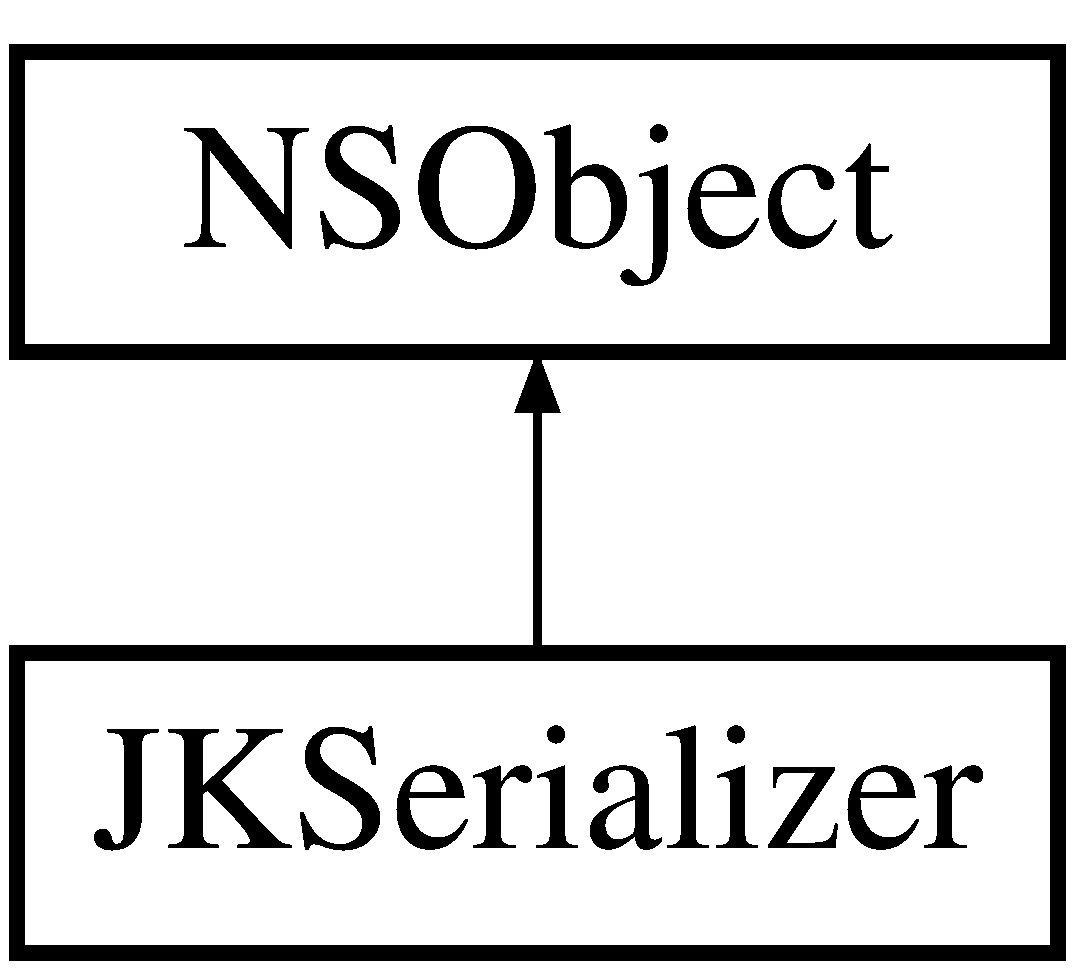
\includegraphics[height=2.000000cm]{interface_j_k_serializer}
\end{center}
\end{figure}
\subsection*{Instance Methods}
\begin{DoxyCompactItemize}
\item 
\hypertarget{interface_j_k_serializer_a87382a040de01c2a3b87c2bec27b8045}{(id) -\/ {\bfseries serialize\+Object\+:options\+:encode\+Option\+:block\+:delegate\+:selector\+:error\+:}}\label{interface_j_k_serializer_a87382a040de01c2a3b87c2bec27b8045}

\item 
\hypertarget{interface_j_k_serializer_a1149913af74980381131cdccf0da8545}{(void) -\/ {\bfseries release\+State}}\label{interface_j_k_serializer_a1149913af74980381131cdccf0da8545}

\end{DoxyCompactItemize}
\subsection*{Class Methods}
\begin{DoxyCompactItemize}
\item 
\hypertarget{interface_j_k_serializer_a87382a040de01c2a3b87c2bec27b8045}{(id) + {\bfseries serialize\+Object\+:options\+:encode\+Option\+:block\+:delegate\+:selector\+:error\+:}}\label{interface_j_k_serializer_a87382a040de01c2a3b87c2bec27b8045}

\end{DoxyCompactItemize}
\subsection*{Protected Attributes}
\begin{DoxyCompactItemize}
\item 
\hypertarget{interface_j_k_serializer_a194502e1f78000add993592a219b5fd7}{\hyperlink{struct_j_k_encode_state}{J\+K\+Encode\+State} $\ast$ {\bfseries encode\+State}}\label{interface_j_k_serializer_a194502e1f78000add993592a219b5fd7}

\end{DoxyCompactItemize}


The documentation for this class was generated from the following file\+:\begin{DoxyCompactItemize}
\item 
J\+S\+O\+N\+Kit/J\+S\+O\+N\+Kit.\+m\end{DoxyCompactItemize}

\hypertarget{struct_j_k_token_cache}{\section{J\+K\+Token\+Cache Struct Reference}
\label{struct_j_k_token_cache}\index{J\+K\+Token\+Cache@{J\+K\+Token\+Cache}}
}
\subsection*{Protected Attributes}
\begin{DoxyCompactItemize}
\item 
\hypertarget{struct_j_k_token_cache_a80b3a1d112b7d798309a71ae3335ab9e}{\hyperlink{struct_j_k_token_cache_item}{J\+K\+Token\+Cache\+Item} $\ast$ {\bfseries items}}\label{struct_j_k_token_cache_a80b3a1d112b7d798309a71ae3335ab9e}

\item 
\hypertarget{struct_j_k_token_cache_a064f4270180ca06ecb5aa14d3b47f2d1}{size\+\_\+t {\bfseries count}}\label{struct_j_k_token_cache_a064f4270180ca06ecb5aa14d3b47f2d1}

\item 
\hypertarget{struct_j_k_token_cache_a02ed24d19e7b1f837d57a4847acee4bb}{unsigned int {\bfseries prng\+\_\+lfsr}}\label{struct_j_k_token_cache_a02ed24d19e7b1f837d57a4847acee4bb}

\item 
\hypertarget{struct_j_k_token_cache_a2cb844821594c94a3d1cd512faa9d66e}{unsigned char {\bfseries age} \mbox{[}J\+K\+\_\+\+C\+A\+C\+H\+E\+\_\+\+S\+L\+O\+T\+S\mbox{]}}\label{struct_j_k_token_cache_a2cb844821594c94a3d1cd512faa9d66e}

\end{DoxyCompactItemize}


The documentation for this struct was generated from the following file\+:\begin{DoxyCompactItemize}
\item 
J\+S\+O\+N\+Kit/J\+S\+O\+N\+Kit.\+m\end{DoxyCompactItemize}

\hypertarget{struct_j_k_token_cache_item}{\section{J\+K\+Token\+Cache\+Item Struct Reference}
\label{struct_j_k_token_cache_item}\index{J\+K\+Token\+Cache\+Item@{J\+K\+Token\+Cache\+Item}}
}
\subsection*{Protected Attributes}
\begin{DoxyCompactItemize}
\item 
\hypertarget{struct_j_k_token_cache_item_a2e20066b2f883735899c4a2b5d0f485c}{void $\ast$ {\bfseries object}}\label{struct_j_k_token_cache_item_a2e20066b2f883735899c4a2b5d0f485c}

\item 
\hypertarget{struct_j_k_token_cache_item_a435cc4ad29e22676dc63f86d57505792}{J\+K\+Hash {\bfseries hash}}\label{struct_j_k_token_cache_item_a435cc4ad29e22676dc63f86d57505792}

\item 
\hypertarget{struct_j_k_token_cache_item_acdee4c0f0ca5d2beb2726d32188cf3cf}{C\+F\+Hash\+Code {\bfseries cf\+Hash}}\label{struct_j_k_token_cache_item_acdee4c0f0ca5d2beb2726d32188cf3cf}

\item 
\hypertarget{struct_j_k_token_cache_item_af207b8177d67ed341eb7d76a8818f599}{size\+\_\+t {\bfseries size}}\label{struct_j_k_token_cache_item_af207b8177d67ed341eb7d76a8818f599}

\item 
\hypertarget{struct_j_k_token_cache_item_a8da7d44fc8a4146563cf907cb4952aea}{unsigned char $\ast$ {\bfseries bytes}}\label{struct_j_k_token_cache_item_a8da7d44fc8a4146563cf907cb4952aea}

\item 
\hypertarget{struct_j_k_token_cache_item_a3966e59525ab02ab68125e7de34b904b}{J\+K\+Value\+Type {\bfseries type}}\label{struct_j_k_token_cache_item_a3966e59525ab02ab68125e7de34b904b}

\end{DoxyCompactItemize}


The documentation for this struct was generated from the following file\+:\begin{DoxyCompactItemize}
\item 
J\+S\+O\+N\+Kit/J\+S\+O\+N\+Kit.\+m\end{DoxyCompactItemize}

\hypertarget{struct_j_k_token_value}{\section{J\+K\+Token\+Value Struct Reference}
\label{struct_j_k_token_value}\index{J\+K\+Token\+Value@{J\+K\+Token\+Value}}
}
\subsection*{Protected Attributes}
\begin{DoxyCompactItemize}
\item 
\hypertarget{struct_j_k_token_value_a3fe09fde3e69bf9f63074714de4f2bfa}{\hyperlink{struct_j_k_const_ptr_range}{J\+K\+Const\+Ptr\+Range} {\bfseries ptr\+Range}}\label{struct_j_k_token_value_a3fe09fde3e69bf9f63074714de4f2bfa}

\item 
\hypertarget{struct_j_k_token_value_a905c992619d59026f2a223b4ee660707}{J\+K\+Value\+Type {\bfseries type}}\label{struct_j_k_token_value_a905c992619d59026f2a223b4ee660707}

\item 
\hypertarget{struct_j_k_token_value_aa377f366a9138439789b6da4fd31418d}{J\+K\+Hash {\bfseries hash}}\label{struct_j_k_token_value_aa377f366a9138439789b6da4fd31418d}

\item 
\hypertarget{struct_j_k_token_value_ad1a9ee37f509c7ca8dae5a7c83ea670a}{\begin{tabbing}
xx\=xx\=xx\=xx\=xx\=xx\=xx\=xx\=xx\=\kill
union \{\\
\hypertarget{union_j_k_token_value_1_1@11_a139d1b7a00b0fd83107b01f0d039a8b1}{\>long long {\bfseries longLongValue}\\
\hypertarget{union_j_k_token_value_1_1@11_ae9399141380d88641a5f48f4ca62fd5d}{\>unsigned long long {\bfseries unsignedLongLongValue}\\
\hypertarget{union_j_k_token_value_1_1@11_ad9f89a50d60de29bce1362a665e08c80}{\>double {\bfseries doubleValue}\\
\} {\bfseries number}}\label{struct_j_k_token_value_ad1a9ee37f509c7ca8dae5a7c83ea670a}
\\

\end{tabbing}\item 
\hypertarget{struct_j_k_token_value_a640704944e9f807c3a9b493bca533480}{\hyperlink{struct_j_k_token_cache_item}{J\+K\+Token\+Cache\+Item} $\ast$ {\bfseries cache\+Item}}\label{struct_j_k_token_value_a640704944e9f807c3a9b493bca533480}

\end{DoxyCompactItemize}


The documentation for this struct was generated from the following file\+:\begin{DoxyCompactItemize}
\item 
J\+S\+O\+N\+Kit/J\+S\+O\+N\+Kit.\+m\end{DoxyCompactItemize}

\hypertarget{class_j_s_o_n_decoder}{\section{J\+S\+O\+N\+Decoder Class Reference}
\label{class_j_s_o_n_decoder}\index{J\+S\+O\+N\+Decoder@{J\+S\+O\+N\+Decoder}}
}


The documentation for this class was generated from the following file\+:\begin{DoxyCompactItemize}
\item 
J\+S\+O\+N\+Kit/J\+S\+O\+N\+Kit.\+m\end{DoxyCompactItemize}

\hypertarget{interface_m_k_number_badge_view}{\section{M\+K\+Number\+Badge\+View Class Reference}
\label{interface_m_k_number_badge_view}\index{M\+K\+Number\+Badge\+View@{M\+K\+Number\+Badge\+View}}
}
Inheritance diagram for M\+K\+Number\+Badge\+View\+:\begin{figure}[H]
\begin{center}
\leavevmode
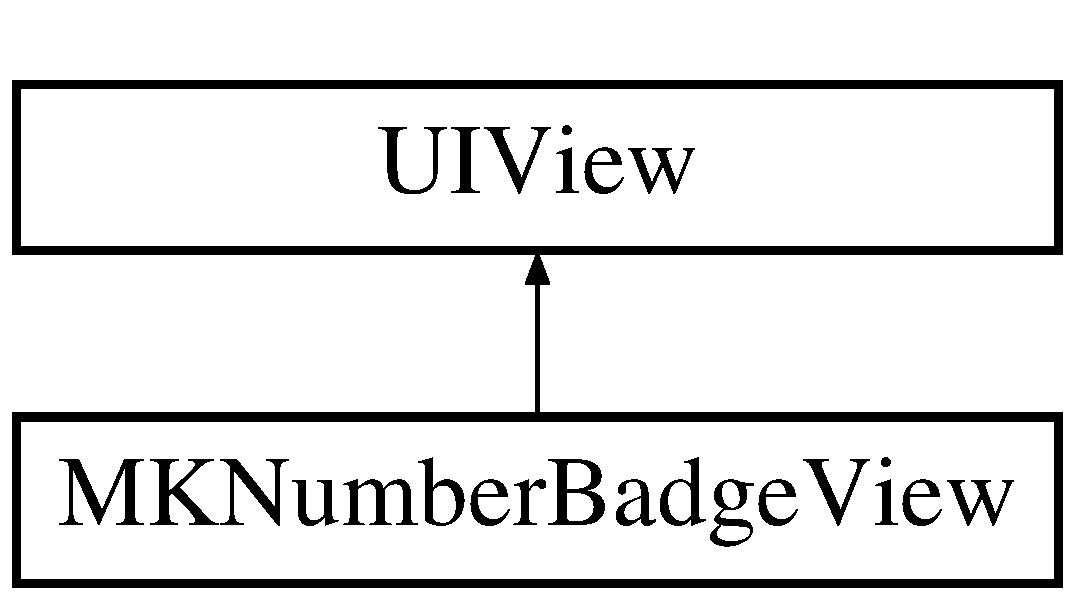
\includegraphics[height=2.000000cm]{interface_m_k_number_badge_view}
\end{center}
\end{figure}
\subsection*{Protected Attributes}
\begin{DoxyCompactItemize}
\item 
\hypertarget{interface_m_k_number_badge_view_a26701201c6ad4c4448dbac97c788bab6}{N\+S\+U\+Integer {\bfseries \+\_\+value}}\label{interface_m_k_number_badge_view_a26701201c6ad4c4448dbac97c788bab6}

\end{DoxyCompactItemize}
\subsection*{Properties}
\begin{DoxyCompactItemize}
\item 
\hypertarget{interface_m_k_number_badge_view_a93007e9e20d2a4fe88ab5d655c4892fa}{N\+S\+String $\ast$ {\bfseries text\+Format}}\label{interface_m_k_number_badge_view_a93007e9e20d2a4fe88ab5d655c4892fa}

\item 
\hypertarget{interface_m_k_number_badge_view_a41e94241b814619c4d3c68c5f1983f42}{C\+G\+Point {\bfseries adjust\+Offset}}\label{interface_m_k_number_badge_view_a41e94241b814619c4d3c68c5f1983f42}

\item 
\hypertarget{interface_m_k_number_badge_view_a83ab7b13a271038405ff1eb8fb1c4f84}{N\+S\+U\+Integer {\bfseries value}}\label{interface_m_k_number_badge_view_a83ab7b13a271038405ff1eb8fb1c4f84}

\item 
\hypertarget{interface_m_k_number_badge_view_a75a7f2d78189f535d71b82c1b7b528f9}{B\+O\+O\+L {\bfseries shadow}}\label{interface_m_k_number_badge_view_a75a7f2d78189f535d71b82c1b7b528f9}

\item 
\hypertarget{interface_m_k_number_badge_view_ad600c1ea35beb68f95ed5c623d65acdc}{C\+G\+Size {\bfseries shadow\+Offset}}\label{interface_m_k_number_badge_view_ad600c1ea35beb68f95ed5c623d65acdc}

\item 
\hypertarget{interface_m_k_number_badge_view_a937e97243d051c408d0bf7396d662f2a}{U\+I\+Color $\ast$ {\bfseries shadow\+Color}}\label{interface_m_k_number_badge_view_a937e97243d051c408d0bf7396d662f2a}

\item 
\hypertarget{interface_m_k_number_badge_view_aff71d7714946dec0355d3673e57713bc}{B\+O\+O\+L {\bfseries shine}}\label{interface_m_k_number_badge_view_aff71d7714946dec0355d3673e57713bc}

\item 
\hypertarget{interface_m_k_number_badge_view_af70f9f4959b90e9b0016c5e38c615fe5}{U\+I\+Font $\ast$ {\bfseries font}}\label{interface_m_k_number_badge_view_af70f9f4959b90e9b0016c5e38c615fe5}

\item 
\hypertarget{interface_m_k_number_badge_view_ad7e0bbe6584a7a1cd9fbd9e4a157d8bc}{U\+I\+Color $\ast$ {\bfseries fill\+Color}}\label{interface_m_k_number_badge_view_ad7e0bbe6584a7a1cd9fbd9e4a157d8bc}

\item 
\hypertarget{interface_m_k_number_badge_view_afcac41773fdb9fdb2b751843ba6cccf5}{U\+I\+Color $\ast$ {\bfseries stroke\+Color}}\label{interface_m_k_number_badge_view_afcac41773fdb9fdb2b751843ba6cccf5}

\item 
\hypertarget{interface_m_k_number_badge_view_afd17106ffa23870714690eaf7cbb71ce}{C\+G\+Float {\bfseries stroke\+Width}}\label{interface_m_k_number_badge_view_afd17106ffa23870714690eaf7cbb71ce}

\item 
\hypertarget{interface_m_k_number_badge_view_ac7651779abe69c876a279be0518aeda8}{U\+I\+Color $\ast$ {\bfseries text\+Color}}\label{interface_m_k_number_badge_view_ac7651779abe69c876a279be0518aeda8}

\item 
\hypertarget{interface_m_k_number_badge_view_aa574e1a1e92655575884f0a1eaf2325f}{N\+S\+Text\+Alignment {\bfseries alignment}}\label{interface_m_k_number_badge_view_aa574e1a1e92655575884f0a1eaf2325f}

\item 
\hypertarget{interface_m_k_number_badge_view_a7d3bb6a28c122cd2347575f3aaf4a3d6}{C\+G\+Size {\bfseries badge\+Size}}\label{interface_m_k_number_badge_view_a7d3bb6a28c122cd2347575f3aaf4a3d6}

\item 
\hypertarget{interface_m_k_number_badge_view_a0a47c8bff71bb346087cf80dbed51cbf}{N\+S\+U\+Integer {\bfseries pad}}\label{interface_m_k_number_badge_view_a0a47c8bff71bb346087cf80dbed51cbf}

\item 
\hypertarget{interface_m_k_number_badge_view_a3f3830b24f219975515c17b2b26bd43b}{B\+O\+O\+L {\bfseries hide\+When\+Zero}}\label{interface_m_k_number_badge_view_a3f3830b24f219975515c17b2b26bd43b}

\end{DoxyCompactItemize}


The documentation for this class was generated from the following files\+:\begin{DoxyCompactItemize}
\item 
Views/\+M\+K\+Number\+Badge/M\+K\+Number\+Badge\+View.\+h\item 
Views/\+M\+K\+Number\+Badge/M\+K\+Number\+Badge\+View.\+m\end{DoxyCompactItemize}

\hypertarget{category_m_k_number_badge_view_07_08}{\section{M\+K\+Number\+Badge\+View() Category Reference}
\label{category_m_k_number_badge_view_07_08}\index{M\+K\+Number\+Badge\+View()@{M\+K\+Number\+Badge\+View()}}
}
\subsection*{Instance Methods}
\begin{DoxyCompactItemize}
\item 
\hypertarget{category_m_k_number_badge_view_07_08_ad9f544f765060e2a097d467dfd94cbde}{(void) -\/ {\bfseries init\+State}}\label{category_m_k_number_badge_view_07_08_ad9f544f765060e2a097d467dfd94cbde}

\item 
\hypertarget{category_m_k_number_badge_view_07_08_accaa33773f40db9748edda849ddf9f51}{(C\+G\+Path\+Ref) -\/ {\bfseries new\+Badge\+Path\+For\+Text\+Size\+:}}\label{category_m_k_number_badge_view_07_08_accaa33773f40db9748edda849ddf9f51}

\end{DoxyCompactItemize}


The documentation for this category was generated from the following file\+:\begin{DoxyCompactItemize}
\item 
Views/\+M\+K\+Number\+Badge/M\+K\+Number\+Badge\+View.\+m\end{DoxyCompactItemize}

\hypertarget{category_n_s_array_07_j_s_o_n_kit_serializing_08}{\section{N\+S\+Array(J\+S\+O\+N\+Kit\+Serializing) Category Reference}
\label{category_n_s_array_07_j_s_o_n_kit_serializing_08}\index{N\+S\+Array(\+J\+S\+O\+N\+Kit\+Serializing)@{N\+S\+Array(\+J\+S\+O\+N\+Kit\+Serializing)}}
}


The documentation for this category was generated from the following file\+:\begin{DoxyCompactItemize}
\item 
J\+S\+O\+N\+Kit/J\+S\+O\+N\+Kit.\+m\end{DoxyCompactItemize}

\hypertarget{category_n_s_data_07_compressor_08}{\section{N\+S\+Data(Compressor) Category Reference}
\label{category_n_s_data_07_compressor_08}\index{N\+S\+Data(\+Compressor)@{N\+S\+Data(\+Compressor)}}
}
\subsection*{Instance Methods}
\begin{DoxyCompactItemize}
\item 
(N\+S\+Data $\ast$) -\/ \hyperlink{category_n_s_data_07_compressor_08_a4da6aae48945349f4aaf30dcc0df7ab8}{uncompress\+Zipped\+Data}
\item 
(N\+S\+Data $\ast$) -\/ \hyperlink{category_n_s_data_07_compressor_08_af347cbf75de636221ff577861d087251}{gzip\+Data}
\end{DoxyCompactItemize}


\subsection{Method Documentation}
\hypertarget{category_n_s_data_07_compressor_08_af347cbf75de636221ff577861d087251}{\index{N\+S\+Data(\+Compressor)@{N\+S\+Data(\+Compressor)}!gzip\+Data@{gzip\+Data}}
\index{gzip\+Data@{gzip\+Data}!N\+S\+Data(\+Compressor)@{N\+S\+Data(\+Compressor)}}
\subsubsection[{gzip\+Data}]{\setlength{\rightskip}{0pt plus 5cm}-\/ (N\+S\+Data $\ast$) gzip\+Data 
\begin{DoxyParamCaption}
{}
\end{DoxyParamCaption}
}}\label{category_n_s_data_07_compressor_08_af347cbf75de636221ff577861d087251}
压缩成gzip格式

\begin{DoxyReturn}{Returns}

\end{DoxyReturn}
\hypertarget{category_n_s_data_07_compressor_08_a4da6aae48945349f4aaf30dcc0df7ab8}{\index{N\+S\+Data(\+Compressor)@{N\+S\+Data(\+Compressor)}!uncompress\+Zipped\+Data@{uncompress\+Zipped\+Data}}
\index{uncompress\+Zipped\+Data@{uncompress\+Zipped\+Data}!N\+S\+Data(\+Compressor)@{N\+S\+Data(\+Compressor)}}
\subsubsection[{uncompress\+Zipped\+Data}]{\setlength{\rightskip}{0pt plus 5cm}-\/ (N\+S\+Data $\ast$) uncompress\+Zipped\+Data 
\begin{DoxyParamCaption}
{}
\end{DoxyParamCaption}
}}\label{category_n_s_data_07_compressor_08_a4da6aae48945349f4aaf30dcc0df7ab8}
解压缩,可以解压zip与gzip压缩过的字符串

\begin{DoxyReturn}{Returns}

\end{DoxyReturn}
解压缩,经过测试,可以解压zip与gzip压缩过的字符串

\begin{DoxyReturn}{Returns}

\end{DoxyReturn}


The documentation for this category was generated from the following files\+:\begin{DoxyCompactItemize}
\item 
Category/N\+S\+Data+\+Compressor.\+h\item 
Category/N\+S\+Data+\+Compressor.\+m\end{DoxyCompactItemize}

\hypertarget{category_n_s_data_07_encryption_08}{\section{N\+S\+Data(Encryption) Category Reference}
\label{category_n_s_data_07_encryption_08}\index{N\+S\+Data(\+Encryption)@{N\+S\+Data(\+Encryption)}}
}
\subsection*{Instance Methods}
\begin{DoxyCompactItemize}
\item 
(N\+S\+Data $\ast$) -\/ \hyperlink{category_n_s_data_07_encryption_08_a7a76eef3c86f0a807607f10bfe6120e9}{A\+E\+S256\+Encrypt\+With\+Key\+:}
\item 
(N\+S\+Data $\ast$) -\/ \hyperlink{category_n_s_data_07_encryption_08_a51d1973dc328b7edf92e18ba000cd304}{A\+E\+S256\+Decrypt\+With\+Key\+:}
\end{DoxyCompactItemize}


\subsection{Method Documentation}
\hypertarget{category_n_s_data_07_encryption_08_a51d1973dc328b7edf92e18ba000cd304}{\index{N\+S\+Data(\+Encryption)@{N\+S\+Data(\+Encryption)}!A\+E\+S256\+Decrypt\+With\+Key\+:@{A\+E\+S256\+Decrypt\+With\+Key\+:}}
\index{A\+E\+S256\+Decrypt\+With\+Key\+:@{A\+E\+S256\+Decrypt\+With\+Key\+:}!N\+S\+Data(\+Encryption)@{N\+S\+Data(\+Encryption)}}
\subsubsection[{A\+E\+S256\+Decrypt\+With\+Key\+:}]{\setlength{\rightskip}{0pt plus 5cm}-\/ (N\+S\+Data $\ast$) A\+E\+S256\+Decrypt\+With\+Key\+: 
\begin{DoxyParamCaption}
\item[{(N\+S\+Data $\ast$)}]{key}
\end{DoxyParamCaption}
}}\label{category_n_s_data_07_encryption_08_a51d1973dc328b7edf92e18ba000cd304}
A\+E\+S解密


\begin{DoxyParams}{Parameters}
{\em key} & 32位的key值,注意key值必须是32位,否则跨平台使用时会有问题\\
\hline
\end{DoxyParams}
\begin{DoxyReturn}{Returns}

\end{DoxyReturn}
\hypertarget{category_n_s_data_07_encryption_08_a7a76eef3c86f0a807607f10bfe6120e9}{\index{N\+S\+Data(\+Encryption)@{N\+S\+Data(\+Encryption)}!A\+E\+S256\+Encrypt\+With\+Key\+:@{A\+E\+S256\+Encrypt\+With\+Key\+:}}
\index{A\+E\+S256\+Encrypt\+With\+Key\+:@{A\+E\+S256\+Encrypt\+With\+Key\+:}!N\+S\+Data(\+Encryption)@{N\+S\+Data(\+Encryption)}}
\subsubsection[{A\+E\+S256\+Encrypt\+With\+Key\+:}]{\setlength{\rightskip}{0pt plus 5cm}-\/ (N\+S\+Data $\ast$) A\+E\+S256\+Encrypt\+With\+Key\+: 
\begin{DoxyParamCaption}
\item[{(N\+S\+Data $\ast$)}]{key}
\end{DoxyParamCaption}
}}\label{category_n_s_data_07_encryption_08_a7a76eef3c86f0a807607f10bfe6120e9}
A\+E\+S加密


\begin{DoxyParams}{Parameters}
{\em key} & 32位的key值,注意key值必须是32位,否则跨平台使用时会有问题\\
\hline
\end{DoxyParams}
\begin{DoxyReturn}{Returns}

\end{DoxyReturn}


The documentation for this category was generated from the following file\+:\begin{DoxyCompactItemize}
\item 
A\+E\+S/N\+S\+Data+\+Encryption.\+h\end{DoxyCompactItemize}

\hypertarget{category_n_s_data_07_j_s_o_n_kit_deserializing_08}{\section{N\+S\+Data(J\+S\+O\+N\+Kit\+Deserializing) Category Reference}
\label{category_n_s_data_07_j_s_o_n_kit_deserializing_08}\index{N\+S\+Data(\+J\+S\+O\+N\+Kit\+Deserializing)@{N\+S\+Data(\+J\+S\+O\+N\+Kit\+Deserializing)}}
}


The documentation for this category was generated from the following file\+:\begin{DoxyCompactItemize}
\item 
J\+S\+O\+N\+Kit/J\+S\+O\+N\+Kit.\+m\end{DoxyCompactItemize}

\hypertarget{category_n_s_dictionary_07_dictionary2_j_s_o_n_08}{\section{N\+S\+Dictionary(Dictionary2\+J\+S\+O\+N) Category Reference}
\label{category_n_s_dictionary_07_dictionary2_j_s_o_n_08}\index{N\+S\+Dictionary(\+Dictionary2\+J\+S\+O\+N)@{N\+S\+Dictionary(\+Dictionary2\+J\+S\+O\+N)}}
}
\subsection*{Instance Methods}
\begin{DoxyCompactItemize}
\item 
(N\+S\+String $\ast$) -\/ \hyperlink{category_n_s_dictionary_07_dictionary2_j_s_o_n_08_ab79f1aebeb2181ce1e3170074126853a}{dictionary2\+J\+S\+O\+N\+:}
\end{DoxyCompactItemize}


\subsection{Method Documentation}
\hypertarget{category_n_s_dictionary_07_dictionary2_j_s_o_n_08_ab79f1aebeb2181ce1e3170074126853a}{\index{N\+S\+Dictionary(\+Dictionary2\+J\+S\+O\+N)@{N\+S\+Dictionary(\+Dictionary2\+J\+S\+O\+N)}!dictionary2\+J\+S\+O\+N\+:@{dictionary2\+J\+S\+O\+N\+:}}
\index{dictionary2\+J\+S\+O\+N\+:@{dictionary2\+J\+S\+O\+N\+:}!N\+S\+Dictionary(\+Dictionary2\+J\+S\+O\+N)@{N\+S\+Dictionary(\+Dictionary2\+J\+S\+O\+N)}}
\subsubsection[{dictionary2\+J\+S\+O\+N\+:}]{\setlength{\rightskip}{0pt plus 5cm}-\/ (N\+S\+String $\ast$) dictionary2\+J\+S\+O\+N\+: 
\begin{DoxyParamCaption}
\item[{(N\+S\+Dictionary$\ast$)}]{target\+Dictionary}
\end{DoxyParamCaption}
}}\label{category_n_s_dictionary_07_dictionary2_j_s_o_n_08_ab79f1aebeb2181ce1e3170074126853a}
字典转换成\+J\+S\+O\+N


\begin{DoxyParams}{Parameters}
{\em target\+Dictionary} & 待转换目标字典\\
\hline
\end{DoxyParams}
\begin{DoxyReturn}{Returns}

\end{DoxyReturn}


The documentation for this category was generated from the following files\+:\begin{DoxyCompactItemize}
\item 
Category/N\+S\+Dictionary+\+Dictionary2\+J\+S\+O\+N.\+h\item 
Category/N\+S\+Dictionary+\+Dictionary2\+J\+S\+O\+N.\+m\end{DoxyCompactItemize}

\hypertarget{category_n_s_dictionary_07_j_s_o_n_kit_serializing_08}{\section{N\+S\+Dictionary(J\+S\+O\+N\+Kit\+Serializing) Category Reference}
\label{category_n_s_dictionary_07_j_s_o_n_kit_serializing_08}\index{N\+S\+Dictionary(\+J\+S\+O\+N\+Kit\+Serializing)@{N\+S\+Dictionary(\+J\+S\+O\+N\+Kit\+Serializing)}}
}


The documentation for this category was generated from the following file\+:\begin{DoxyCompactItemize}
\item 
J\+S\+O\+N\+Kit/J\+S\+O\+N\+Kit.\+m\end{DoxyCompactItemize}

\hypertarget{category_n_s_object_07_class_name_08}{\section{N\+S\+Object(Class\+Name) Category Reference}
\label{category_n_s_object_07_class_name_08}\index{N\+S\+Object(\+Class\+Name)@{N\+S\+Object(\+Class\+Name)}}
}
\subsection*{Class Methods}
\begin{DoxyCompactItemize}
\item 
(N\+S\+String $\ast$) + \hyperlink{category_n_s_object_07_class_name_08_a1a88504ee5249caa01c45dabaa8dda66}{class\+Name}
\end{DoxyCompactItemize}


\subsection{Method Documentation}
\hypertarget{category_n_s_object_07_class_name_08_a1a88504ee5249caa01c45dabaa8dda66}{\index{N\+S\+Object(\+Class\+Name)@{N\+S\+Object(\+Class\+Name)}!class\+Name@{class\+Name}}
\index{class\+Name@{class\+Name}!N\+S\+Object(\+Class\+Name)@{N\+S\+Object(\+Class\+Name)}}
\subsubsection[{class\+Name}]{\setlength{\rightskip}{0pt plus 5cm}+ (N\+S\+String $\ast$) class\+Name 
\begin{DoxyParamCaption}
{}
\end{DoxyParamCaption}
}}\label{category_n_s_object_07_class_name_08_a1a88504ee5249caa01c45dabaa8dda66}
将对象类名称转换成字符串

\begin{DoxyReturn}{Returns}

\end{DoxyReturn}


The documentation for this category was generated from the following files\+:\begin{DoxyCompactItemize}
\item 
Category/N\+S\+Object+\+Class\+Name.\+h\item 
Category/N\+S\+Object+\+Class\+Name.\+m\end{DoxyCompactItemize}

\hypertarget{category_n_s_string_07_a_e_s256_encrypt_08}{\section{N\+S\+String(A\+E\+S256\+Encrypt) Category Reference}
\label{category_n_s_string_07_a_e_s256_encrypt_08}\index{N\+S\+String(\+A\+E\+S256\+Encrypt)@{N\+S\+String(\+A\+E\+S256\+Encrypt)}}
}
\subsection*{Instance Methods}
\begin{DoxyCompactItemize}
\item 
(N\+S\+String $\ast$) -\/ \hyperlink{category_n_s_string_07_a_e_s256_encrypt_08_a8d40511a483a7d1a15ef0565dfa3ad7c}{A\+E\+S256\+Encrypt\+:}
\item 
(N\+S\+String $\ast$) -\/ \hyperlink{category_n_s_string_07_a_e_s256_encrypt_08_afcf4895e16d68f55b897f0b925f2dd56}{A\+E\+S256\+Decrypt\+:}
\end{DoxyCompactItemize}


\subsection{Method Documentation}
\hypertarget{category_n_s_string_07_a_e_s256_encrypt_08_afcf4895e16d68f55b897f0b925f2dd56}{\index{N\+S\+String(\+A\+E\+S256\+Encrypt)@{N\+S\+String(\+A\+E\+S256\+Encrypt)}!A\+E\+S256\+Decrypt\+:@{A\+E\+S256\+Decrypt\+:}}
\index{A\+E\+S256\+Decrypt\+:@{A\+E\+S256\+Decrypt\+:}!N\+S\+String(\+A\+E\+S256\+Encrypt)@{N\+S\+String(\+A\+E\+S256\+Encrypt)}}
\subsubsection[{A\+E\+S256\+Decrypt\+:}]{\setlength{\rightskip}{0pt plus 5cm}-\/ (N\+S\+String $\ast$) A\+E\+S256\+Decrypt\+: 
\begin{DoxyParamCaption}
\item[{(N\+S\+String$\ast$)}]{key}
\end{DoxyParamCaption}
}}\label{category_n_s_string_07_a_e_s256_encrypt_08_afcf4895e16d68f55b897f0b925f2dd56}
A\+E\+S 256解密


\begin{DoxyParams}{Parameters}
{\em key} & 32位的key值,注意key值必须是32位,否则跨平台使用时会有问题\\
\hline
\end{DoxyParams}
\begin{DoxyReturn}{Returns}

\end{DoxyReturn}
\hypertarget{category_n_s_string_07_a_e_s256_encrypt_08_a8d40511a483a7d1a15ef0565dfa3ad7c}{\index{N\+S\+String(\+A\+E\+S256\+Encrypt)@{N\+S\+String(\+A\+E\+S256\+Encrypt)}!A\+E\+S256\+Encrypt\+:@{A\+E\+S256\+Encrypt\+:}}
\index{A\+E\+S256\+Encrypt\+:@{A\+E\+S256\+Encrypt\+:}!N\+S\+String(\+A\+E\+S256\+Encrypt)@{N\+S\+String(\+A\+E\+S256\+Encrypt)}}
\subsubsection[{A\+E\+S256\+Encrypt\+:}]{\setlength{\rightskip}{0pt plus 5cm}-\/ (N\+S\+String $\ast$) A\+E\+S256\+Encrypt\+: 
\begin{DoxyParamCaption}
\item[{(N\+S\+String$\ast$)}]{key}
\end{DoxyParamCaption}
}}\label{category_n_s_string_07_a_e_s256_encrypt_08_a8d40511a483a7d1a15ef0565dfa3ad7c}
A\+E\+S 256加密


\begin{DoxyParams}{Parameters}
{\em key} & 32位的key值,注意key值必须是32位,否则跨平台使用时会有问题\\
\hline
\end{DoxyParams}
\begin{DoxyReturn}{Returns}

\end{DoxyReturn}


The documentation for this category was generated from the following files\+:\begin{DoxyCompactItemize}
\item 
A\+E\+S/N\+S\+String+\+A\+E\+S256\+Encrypt.\+h\item 
A\+E\+S/N\+S\+String+\+A\+E\+S256\+Encrypt.\+m\end{DoxyCompactItemize}

\hypertarget{category_n_s_string_07_j_s_o_n_kit_deserializing_08}{\section{N\+S\+String(J\+S\+O\+N\+Kit\+Deserializing) Category Reference}
\label{category_n_s_string_07_j_s_o_n_kit_deserializing_08}\index{N\+S\+String(\+J\+S\+O\+N\+Kit\+Deserializing)@{N\+S\+String(\+J\+S\+O\+N\+Kit\+Deserializing)}}
}


The documentation for this category was generated from the following file\+:\begin{DoxyCompactItemize}
\item 
J\+S\+O\+N\+Kit/J\+S\+O\+N\+Kit.\+m\end{DoxyCompactItemize}

\hypertarget{category_n_s_string_07_j_s_o_n_kit_serializing_08}{\section{N\+S\+String(J\+S\+O\+N\+Kit\+Serializing) Category Reference}
\label{category_n_s_string_07_j_s_o_n_kit_serializing_08}\index{N\+S\+String(\+J\+S\+O\+N\+Kit\+Serializing)@{N\+S\+String(\+J\+S\+O\+N\+Kit\+Serializing)}}
}


The documentation for this category was generated from the following file\+:\begin{DoxyCompactItemize}
\item 
J\+S\+O\+N\+Kit/J\+S\+O\+N\+Kit.\+m\end{DoxyCompactItemize}

\hypertarget{category_n_s_string_07_trim_08}{\section{N\+S\+String(Trim) Category Reference}
\label{category_n_s_string_07_trim_08}\index{N\+S\+String(\+Trim)@{N\+S\+String(\+Trim)}}
}
\subsection*{Instance Methods}
\begin{DoxyCompactItemize}
\item 
(N\+S\+String $\ast$) -\/ \hyperlink{category_n_s_string_07_trim_08_a3332817f0b6b24998b6f23c1161e82a0}{trim}
\end{DoxyCompactItemize}


\subsection{Method Documentation}
\hypertarget{category_n_s_string_07_trim_08_a3332817f0b6b24998b6f23c1161e82a0}{\index{N\+S\+String(\+Trim)@{N\+S\+String(\+Trim)}!trim@{trim}}
\index{trim@{trim}!N\+S\+String(\+Trim)@{N\+S\+String(\+Trim)}}
\subsubsection[{trim}]{\setlength{\rightskip}{0pt plus 5cm}-\/ (N\+S\+String $\ast$) trim 
\begin{DoxyParamCaption}
{}
\end{DoxyParamCaption}
}}\label{category_n_s_string_07_trim_08_a3332817f0b6b24998b6f23c1161e82a0}
去除首尾空格

\begin{DoxyReturn}{Returns}

\end{DoxyReturn}


The documentation for this category was generated from the following files\+:\begin{DoxyCompactItemize}
\item 
Category/N\+S\+String+\+Trim.\+h\item 
Category/N\+S\+String+\+Trim.\+m\end{DoxyCompactItemize}

\hypertarget{category_n_s_string_07_u_r_l_08}{\section{N\+S\+String(U\+R\+L) Category Reference}
\label{category_n_s_string_07_u_r_l_08}\index{N\+S\+String(\+U\+R\+L)@{N\+S\+String(\+U\+R\+L)}}
}
\subsection*{Instance Methods}
\begin{DoxyCompactItemize}
\item 
(N\+S\+String $\ast$) -\/ \hyperlink{category_n_s_string_07_u_r_l_08_a8148309a8c2a055ee184b589aecfa02e}{U\+R\+L\+Encoded\+String}
\end{DoxyCompactItemize}


\subsection{Method Documentation}
\hypertarget{category_n_s_string_07_u_r_l_08_a8148309a8c2a055ee184b589aecfa02e}{\index{N\+S\+String(\+U\+R\+L)@{N\+S\+String(\+U\+R\+L)}!U\+R\+L\+Encoded\+String@{U\+R\+L\+Encoded\+String}}
\index{U\+R\+L\+Encoded\+String@{U\+R\+L\+Encoded\+String}!N\+S\+String(\+U\+R\+L)@{N\+S\+String(\+U\+R\+L)}}
\subsubsection[{U\+R\+L\+Encoded\+String}]{\setlength{\rightskip}{0pt plus 5cm}-\/ (N\+S\+String $\ast$) U\+R\+L\+Encoded\+String 
\begin{DoxyParamCaption}
{}
\end{DoxyParamCaption}
}}\label{category_n_s_string_07_u_r_l_08_a8148309a8c2a055ee184b589aecfa02e}
将\+U\+R\+L中的非拉丁字符转换成全拉丁字符

\begin{DoxyReturn}{Returns}

\end{DoxyReturn}


The documentation for this category was generated from the following files\+:\begin{DoxyCompactItemize}
\item 
Category/N\+S\+String+\+U\+R\+L.\+h\item 
Category/N\+S\+String+\+U\+R\+L.\+m\end{DoxyCompactItemize}

\hypertarget{category_u_i_alert_view_07_block_08}{\section{U\+I\+Alert\+View(Block) Category Reference}
\label{category_u_i_alert_view_07_block_08}\index{U\+I\+Alert\+View(\+Block)@{U\+I\+Alert\+View(\+Block)}}
}
\subsection*{Instance Methods}
\begin{DoxyCompactItemize}
\item 
(void) -\/ \hyperlink{category_u_i_alert_view_07_block_08_a911f8b6abd31cc0b95b98aff88de9515}{show\+Alert\+View\+With\+Complete\+Block\+:}
\end{DoxyCompactItemize}
\subsection*{Protected Types}
\begin{DoxyCompactItemize}
\item 
typedef void($^\wedge$ \hyperlink{category_u_i_alert_view_07_block_08_ab250b3fbf44082caf18f9ca597e5dcc5}{Complete\+Block} )(N\+S\+Integer button\+Index)
\end{DoxyCompactItemize}


\subsection{Member Typedef Documentation}
\hypertarget{category_u_i_alert_view_07_block_08_ab250b3fbf44082caf18f9ca597e5dcc5}{\index{U\+I\+Alert\+View(\+Block)@{U\+I\+Alert\+View(\+Block)}!Complete\+Block@{Complete\+Block}}
\index{Complete\+Block@{Complete\+Block}!U\+I\+Alert\+View(\+Block)@{U\+I\+Alert\+View(\+Block)}}
\subsubsection[{Complete\+Block}]{\setlength{\rightskip}{0pt plus 5cm}-\/ (typedef void($^\wedge$ Complete\+Block)(N\+S\+Integer button\+Index))\hspace{0.3cm}{\ttfamily [protected]}}}\label{category_u_i_alert_view_07_block_08_ab250b3fbf44082caf18f9ca597e5dcc5}
定义一个点击弹出按钮后的回调block


\begin{DoxyParams}{Parameters}
{\em button\+Index} & 点击按钮的index \\
\hline
\end{DoxyParams}


\subsection{Method Documentation}
\hypertarget{category_u_i_alert_view_07_block_08_a911f8b6abd31cc0b95b98aff88de9515}{\index{U\+I\+Alert\+View(\+Block)@{U\+I\+Alert\+View(\+Block)}!show\+Alert\+View\+With\+Complete\+Block\+:@{show\+Alert\+View\+With\+Complete\+Block\+:}}
\index{show\+Alert\+View\+With\+Complete\+Block\+:@{show\+Alert\+View\+With\+Complete\+Block\+:}!U\+I\+Alert\+View(\+Block)@{U\+I\+Alert\+View(\+Block)}}
\subsubsection[{show\+Alert\+View\+With\+Complete\+Block\+:}]{\setlength{\rightskip}{0pt plus 5cm}-\/ (void) show\+Alert\+View\+With\+Complete\+Block\+: 
\begin{DoxyParamCaption}
\item[{({\bf Complete\+Block})}]{block}
\end{DoxyParamCaption}
}}\label{category_u_i_alert_view_07_block_08_a911f8b6abd31cc0b95b98aff88de9515}
用\+Block的方式回调,这时候会默认用self作为\+Delegate


\begin{DoxyParams}{Parameters}
{\em block} & Complete\+Block \\
\hline
\end{DoxyParams}
1 创建关联(源对象,关键字,关联的对象和一个关联策略。) 2 关键字是一个void类型的指针。每一个关联的关键字必须是唯一的。通常都是会采用静态变量来作为关键字。 3 关联策略表明了相关的对象是通过赋值,保留引用还是复制的方式进行关联的;关联是原子的还是非原子的。这里的关联策略和声明属性时的很类似。

The documentation for this category was generated from the following files\+:\begin{DoxyCompactItemize}
\item 
Category/U\+I\+Alert\+View+\+Block.\+h\item 
Category/U\+I\+Alert\+View+\+Block.\+m\end{DoxyCompactItemize}

\hypertarget{category_u_i_color_07_u_i_color_from_hex_08}{\section{U\+I\+Color(U\+I\+Color\+From\+Hex) Category Reference}
\label{category_u_i_color_07_u_i_color_from_hex_08}\index{U\+I\+Color(\+U\+I\+Color\+From\+Hex)@{U\+I\+Color(\+U\+I\+Color\+From\+Hex)}}
}
\subsection*{Class Methods}
\begin{DoxyCompactItemize}
\item 
(U\+I\+Color $\ast$) + \hyperlink{category_u_i_color_07_u_i_color_from_hex_08_a50bab54fcbceb58002351586a9303761}{color\+With\+Hex\+:alpha\+:}
\item 
(U\+I\+Color $\ast$) + \hyperlink{category_u_i_color_07_u_i_color_from_hex_08_a8ca14e16bdd7ec892aa32c5592967d0d}{color\+With\+Hex\+:}
\item 
(U\+I\+Color $\ast$) + \hyperlink{category_u_i_color_07_u_i_color_from_hex_08_acf23a77c8281f2cde755a982339bf527}{white\+Color\+With\+Alpha\+:}
\item 
(U\+I\+Color $\ast$) + \hyperlink{category_u_i_color_07_u_i_color_from_hex_08_a4531f319ff3624e60d6cb0658597c1c4}{black\+Color\+With\+Alpha\+:}
\end{DoxyCompactItemize}


\subsection{Method Documentation}
\hypertarget{category_u_i_color_07_u_i_color_from_hex_08_a4531f319ff3624e60d6cb0658597c1c4}{\index{U\+I\+Color(\+U\+I\+Color\+From\+Hex)@{U\+I\+Color(\+U\+I\+Color\+From\+Hex)}!black\+Color\+With\+Alpha\+:@{black\+Color\+With\+Alpha\+:}}
\index{black\+Color\+With\+Alpha\+:@{black\+Color\+With\+Alpha\+:}!U\+I\+Color(\+U\+I\+Color\+From\+Hex)@{U\+I\+Color(\+U\+I\+Color\+From\+Hex)}}
\subsubsection[{black\+Color\+With\+Alpha\+:}]{\setlength{\rightskip}{0pt plus 5cm}+ (U\+I\+Color $\ast$) black\+Color\+With\+Alpha\+: 
\begin{DoxyParamCaption}
\item[{(C\+G\+Float)}]{alpha\+Value}
\end{DoxyParamCaption}
}}\label{category_u_i_color_07_u_i_color_from_hex_08_a4531f319ff3624e60d6cb0658597c1c4}
颜色为黑色时的透明度设置


\begin{DoxyParams}{Parameters}
{\em alpha\+Value} & 透明度\\
\hline
\end{DoxyParams}
\begin{DoxyReturn}{Returns}

\end{DoxyReturn}
\hypertarget{category_u_i_color_07_u_i_color_from_hex_08_a8ca14e16bdd7ec892aa32c5592967d0d}{\index{U\+I\+Color(\+U\+I\+Color\+From\+Hex)@{U\+I\+Color(\+U\+I\+Color\+From\+Hex)}!color\+With\+Hex\+:@{color\+With\+Hex\+:}}
\index{color\+With\+Hex\+:@{color\+With\+Hex\+:}!U\+I\+Color(\+U\+I\+Color\+From\+Hex)@{U\+I\+Color(\+U\+I\+Color\+From\+Hex)}}
\subsubsection[{color\+With\+Hex\+:}]{\setlength{\rightskip}{0pt plus 5cm}+ (U\+I\+Color $\ast$) color\+With\+Hex\+: 
\begin{DoxyParamCaption}
\item[{(N\+S\+Integer)}]{hex\+Value}
\end{DoxyParamCaption}
}}\label{category_u_i_color_07_u_i_color_from_hex_08_a8ca14e16bdd7ec892aa32c5592967d0d}
以6位十六进制的形式表示颜色


\begin{DoxyParams}{Parameters}
{\em hex\+Value} & 6位十六进制数:0x000000 $\sim$ 0xffffff\\
\hline
\end{DoxyParams}
\begin{DoxyReturn}{Returns}

\end{DoxyReturn}
\hypertarget{category_u_i_color_07_u_i_color_from_hex_08_a50bab54fcbceb58002351586a9303761}{\index{U\+I\+Color(\+U\+I\+Color\+From\+Hex)@{U\+I\+Color(\+U\+I\+Color\+From\+Hex)}!color\+With\+Hex\+:alpha\+:@{color\+With\+Hex\+:alpha\+:}}
\index{color\+With\+Hex\+:alpha\+:@{color\+With\+Hex\+:alpha\+:}!U\+I\+Color(\+U\+I\+Color\+From\+Hex)@{U\+I\+Color(\+U\+I\+Color\+From\+Hex)}}
\subsubsection[{color\+With\+Hex\+:alpha\+:}]{\setlength{\rightskip}{0pt plus 5cm}+ (U\+I\+Color $\ast$) {\bf color\+With\+Hex\+:} 
\begin{DoxyParamCaption}
\item[{(N\+S\+Integer)}]{hex\+Value}
\item[{alpha:(C\+G\+Float)}]{alpha\+Value}
\end{DoxyParamCaption}
}}\label{category_u_i_color_07_u_i_color_from_hex_08_a50bab54fcbceb58002351586a9303761}
以6位十六进制的形式表示颜色,并且可以设置该颜色的透明度


\begin{DoxyParams}{Parameters}
{\em hex\+Value} & 6位十六进制数:0x000000 $\sim$ 0xffffff \\
\hline
{\em alpha\+Value} & 透明度\\
\hline
\end{DoxyParams}
\begin{DoxyReturn}{Returns}

\end{DoxyReturn}
\hypertarget{category_u_i_color_07_u_i_color_from_hex_08_acf23a77c8281f2cde755a982339bf527}{\index{U\+I\+Color(\+U\+I\+Color\+From\+Hex)@{U\+I\+Color(\+U\+I\+Color\+From\+Hex)}!white\+Color\+With\+Alpha\+:@{white\+Color\+With\+Alpha\+:}}
\index{white\+Color\+With\+Alpha\+:@{white\+Color\+With\+Alpha\+:}!U\+I\+Color(\+U\+I\+Color\+From\+Hex)@{U\+I\+Color(\+U\+I\+Color\+From\+Hex)}}
\subsubsection[{white\+Color\+With\+Alpha\+:}]{\setlength{\rightskip}{0pt plus 5cm}+ (U\+I\+Color $\ast$) white\+Color\+With\+Alpha\+: 
\begin{DoxyParamCaption}
\item[{(C\+G\+Float)}]{alpha\+Value}
\end{DoxyParamCaption}
}}\label{category_u_i_color_07_u_i_color_from_hex_08_acf23a77c8281f2cde755a982339bf527}
颜色为白色时的透明度设置


\begin{DoxyParams}{Parameters}
{\em alpha\+Value} & 透明度\\
\hline
\end{DoxyParams}
\begin{DoxyReturn}{Returns}

\end{DoxyReturn}


The documentation for this category was generated from the following files\+:\begin{DoxyCompactItemize}
\item 
Category/U\+I\+Color+\+U\+I\+Color\+From\+Hex.\+h\item 
Category/U\+I\+Color+\+U\+I\+Color\+From\+Hex.\+m\end{DoxyCompactItemize}

\hypertarget{category_u_i_image_07_circle_image_08}{\section{U\+I\+Image(Circle\+Image) Category Reference}
\label{category_u_i_image_07_circle_image_08}\index{U\+I\+Image(\+Circle\+Image)@{U\+I\+Image(\+Circle\+Image)}}
}
\subsection*{Instance Methods}
\begin{DoxyCompactItemize}
\item 
(U\+I\+Image $\ast$) -\/ \hyperlink{category_u_i_image_07_circle_image_08_a0a76bddad3eacc24d0fcd7dc50812afb}{circle\+Image\+With\+Inset\+:}
\end{DoxyCompactItemize}


\subsection{Method Documentation}
\hypertarget{category_u_i_image_07_circle_image_08_a0a76bddad3eacc24d0fcd7dc50812afb}{\index{U\+I\+Image(\+Circle\+Image)@{U\+I\+Image(\+Circle\+Image)}!circle\+Image\+With\+Inset\+:@{circle\+Image\+With\+Inset\+:}}
\index{circle\+Image\+With\+Inset\+:@{circle\+Image\+With\+Inset\+:}!U\+I\+Image(\+Circle\+Image)@{U\+I\+Image(\+Circle\+Image)}}
\subsubsection[{circle\+Image\+With\+Inset\+:}]{\setlength{\rightskip}{0pt plus 5cm}-\/ (U\+I\+Image $\ast$) circle\+Image\+With\+Inset\+: 
\begin{DoxyParamCaption}
\item[{(C\+G\+Float)}]{inset}
\end{DoxyParamCaption}
}}\label{category_u_i_image_07_circle_image_08_a0a76bddad3eacc24d0fcd7dc50812afb}
制造圆形图片


\begin{DoxyParams}{Parameters}
{\em inset} & 会根据原始图的最大半径扣除inset值来画园\\
\hline
\end{DoxyParams}
\begin{DoxyReturn}{Returns}

\end{DoxyReturn}


The documentation for this category was generated from the following files\+:\begin{DoxyCompactItemize}
\item 
Category/U\+I\+Image+\+Circle\+Image.\+h\item 
Category/U\+I\+Image+\+Circle\+Image.\+m\end{DoxyCompactItemize}

\hypertarget{category_u_i_image_07_u_i_image_from_u_i_color_08}{\section{U\+I\+Image(U\+I\+Image\+From\+U\+I\+Color) Category Reference}
\label{category_u_i_image_07_u_i_image_from_u_i_color_08}\index{U\+I\+Image(\+U\+I\+Image\+From\+U\+I\+Color)@{U\+I\+Image(\+U\+I\+Image\+From\+U\+I\+Color)}}
}
\subsection*{Class Methods}
\begin{DoxyCompactItemize}
\item 
(U\+I\+Image $\ast$) + \hyperlink{category_u_i_image_07_u_i_image_from_u_i_color_08_a9a93e47a000ed1883dcf81bf78afecf6}{init\+Image\+With\+U\+I\+Color\+:}
\item 
(U\+I\+Image $\ast$) + \hyperlink{category_u_i_image_07_u_i_image_from_u_i_color_08_ac2cdb9fd057a153936f4a77b5b690eea}{init\+Image\+With\+U\+I\+Color\+:and\+Size\+:}
\end{DoxyCompactItemize}


\subsection{Method Documentation}
\hypertarget{category_u_i_image_07_u_i_image_from_u_i_color_08_a9a93e47a000ed1883dcf81bf78afecf6}{\index{U\+I\+Image(\+U\+I\+Image\+From\+U\+I\+Color)@{U\+I\+Image(\+U\+I\+Image\+From\+U\+I\+Color)}!init\+Image\+With\+U\+I\+Color\+:@{init\+Image\+With\+U\+I\+Color\+:}}
\index{init\+Image\+With\+U\+I\+Color\+:@{init\+Image\+With\+U\+I\+Color\+:}!U\+I\+Image(\+U\+I\+Image\+From\+U\+I\+Color)@{U\+I\+Image(\+U\+I\+Image\+From\+U\+I\+Color)}}
\subsubsection[{init\+Image\+With\+U\+I\+Color\+:}]{\setlength{\rightskip}{0pt plus 5cm}+ (U\+I\+Image $\ast$) init\+Image\+With\+U\+I\+Color\+: 
\begin{DoxyParamCaption}
\item[{(U\+I\+Color $\ast$)}]{color}
\end{DoxyParamCaption}
}}\label{category_u_i_image_07_u_i_image_from_u_i_color_08_a9a93e47a000ed1883dcf81bf78afecf6}
以颜色来设置图片


\begin{DoxyParams}{Parameters}
{\em color} & 设置颜色\\
\hline
\end{DoxyParams}
\begin{DoxyReturn}{Returns}

\end{DoxyReturn}
\hypertarget{category_u_i_image_07_u_i_image_from_u_i_color_08_ac2cdb9fd057a153936f4a77b5b690eea}{\index{U\+I\+Image(\+U\+I\+Image\+From\+U\+I\+Color)@{U\+I\+Image(\+U\+I\+Image\+From\+U\+I\+Color)}!init\+Image\+With\+U\+I\+Color\+:and\+Size\+:@{init\+Image\+With\+U\+I\+Color\+:and\+Size\+:}}
\index{init\+Image\+With\+U\+I\+Color\+:and\+Size\+:@{init\+Image\+With\+U\+I\+Color\+:and\+Size\+:}!U\+I\+Image(\+U\+I\+Image\+From\+U\+I\+Color)@{U\+I\+Image(\+U\+I\+Image\+From\+U\+I\+Color)}}
\subsubsection[{init\+Image\+With\+U\+I\+Color\+:and\+Size\+:}]{\setlength{\rightskip}{0pt plus 5cm}+ (U\+I\+Image $\ast$) {\bf init\+Image\+With\+U\+I\+Color\+:} 
\begin{DoxyParamCaption}
\item[{(U\+I\+Color $\ast$)}]{color}
\item[{andSize:(C\+G\+Size)}]{size}
\end{DoxyParamCaption}
}}\label{category_u_i_image_07_u_i_image_from_u_i_color_08_ac2cdb9fd057a153936f4a77b5b690eea}
以颜色来设置图片,并设置图片尺寸


\begin{DoxyParams}{Parameters}
{\em color} & 设置颜色 \\
\hline
{\em size} & 图片尺寸\\
\hline
\end{DoxyParams}
\begin{DoxyReturn}{Returns}

\end{DoxyReturn}


The documentation for this category was generated from the following files\+:\begin{DoxyCompactItemize}
\item 
Category/U\+I\+Image+\+U\+I\+Image\+From\+U\+I\+Color.\+h\item 
Category/U\+I\+Image+\+U\+I\+Image\+From\+U\+I\+Color.\+m\end{DoxyCompactItemize}

\hypertarget{category_u_i_image_07_u_i_rounded_rect_image_08}{\section{U\+I\+Image(U\+I\+Rounded\+Rect\+Image) Category Reference}
\label{category_u_i_image_07_u_i_rounded_rect_image_08}\index{U\+I\+Image(\+U\+I\+Rounded\+Rect\+Image)@{U\+I\+Image(\+U\+I\+Rounded\+Rect\+Image)}}
}
\subsection*{Instance Methods}
\begin{DoxyCompactItemize}
\item 
(U\+I\+Image $\ast$) -\/ \hyperlink{category_u_i_image_07_u_i_rounded_rect_image_08_a3cf89cb2d3de32d197d0c0d84e01a5b4}{create\+Rounded\+Rect\+Image\+:size\+:}
\end{DoxyCompactItemize}


\subsection{Method Documentation}
\hypertarget{category_u_i_image_07_u_i_rounded_rect_image_08_a3cf89cb2d3de32d197d0c0d84e01a5b4}{\index{U\+I\+Image(\+U\+I\+Rounded\+Rect\+Image)@{U\+I\+Image(\+U\+I\+Rounded\+Rect\+Image)}!create\+Rounded\+Rect\+Image\+:size\+:@{create\+Rounded\+Rect\+Image\+:size\+:}}
\index{create\+Rounded\+Rect\+Image\+:size\+:@{create\+Rounded\+Rect\+Image\+:size\+:}!U\+I\+Image(\+U\+I\+Rounded\+Rect\+Image)@{U\+I\+Image(\+U\+I\+Rounded\+Rect\+Image)}}
\subsubsection[{create\+Rounded\+Rect\+Image\+:size\+:}]{\setlength{\rightskip}{0pt plus 5cm}-\/ (U\+I\+Image $\ast$) create\+Rounded\+Rect\+Image\+: 
\begin{DoxyParamCaption}
\item[{(U\+I\+Image$\ast$)}]{image}
\item[{size:(C\+G\+Size)}]{size}
\end{DoxyParamCaption}
}}\label{category_u_i_image_07_u_i_rounded_rect_image_08_a3cf89cb2d3de32d197d0c0d84e01a5b4}
将矩形图片设置成圆角图片,尺寸可以自定义


\begin{DoxyParams}{Parameters}
{\em image} & 待设置图片 \\
\hline
{\em size} & 自定义尺寸\\
\hline
\end{DoxyParams}
\begin{DoxyReturn}{Returns}

\end{DoxyReturn}


The documentation for this category was generated from the following files\+:\begin{DoxyCompactItemize}
\item 
Category/U\+I\+Image+\+U\+I\+Rounded\+Rect\+Image.\+h\item 
Category/U\+I\+Image+\+U\+I\+Rounded\+Rect\+Image.\+m\end{DoxyCompactItemize}

\hypertarget{category_u_i_navigation_bar_07_customize_08}{\section{U\+I\+Navigation\+Bar(Customize) Category Reference}
\label{category_u_i_navigation_bar_07_customize_08}\index{U\+I\+Navigation\+Bar(\+Customize)@{U\+I\+Navigation\+Bar(\+Customize)}}
}
\subsection*{Instance Methods}
\begin{DoxyCompactItemize}
\item 
(void) -\/ \hyperlink{category_u_i_navigation_bar_07_customize_08_aa73b84df91f31fae792d932e263087e1}{set\+Background\+Color\+:}
\item 
(void) -\/ \hyperlink{category_u_i_navigation_bar_07_customize_08_adfc2d75e883e6303205bbd634818a887}{set\+Default\+Background\+Color}
\item 
(void) -\/ \hyperlink{category_u_i_navigation_bar_07_customize_08_a2d262b83c3b5b90a060d2bd58f060c99}{set\+Bar\+Button\+Item\+Color\+:}
\item 
(void) -\/ \hyperlink{category_u_i_navigation_bar_07_customize_08_ac55b9e69404090fa0ca783e017ce705f}{set\+Title\+Color\+:}
\end{DoxyCompactItemize}


\subsection{Method Documentation}
\hypertarget{category_u_i_navigation_bar_07_customize_08_aa73b84df91f31fae792d932e263087e1}{\index{U\+I\+Navigation\+Bar(\+Customize)@{U\+I\+Navigation\+Bar(\+Customize)}!set\+Background\+Color\+:@{set\+Background\+Color\+:}}
\index{set\+Background\+Color\+:@{set\+Background\+Color\+:}!U\+I\+Navigation\+Bar(\+Customize)@{U\+I\+Navigation\+Bar(\+Customize)}}
\subsubsection[{set\+Background\+Color\+:}]{\setlength{\rightskip}{0pt plus 5cm}-\/ (void) set\+Background\+Color\+: 
\begin{DoxyParamCaption}
\item[{(N\+S\+Integer)}]{color}
\end{DoxyParamCaption}
}}\label{category_u_i_navigation_bar_07_customize_08_aa73b84df91f31fae792d932e263087e1}
设置背景颜色(16进制颜色)


\begin{DoxyParams}{Parameters}
{\em color} & 16进制颜色,例如0x\+A\+A\+B\+B\+C\+C \\
\hline
\end{DoxyParams}
\hypertarget{category_u_i_navigation_bar_07_customize_08_a2d262b83c3b5b90a060d2bd58f060c99}{\index{U\+I\+Navigation\+Bar(\+Customize)@{U\+I\+Navigation\+Bar(\+Customize)}!set\+Bar\+Button\+Item\+Color\+:@{set\+Bar\+Button\+Item\+Color\+:}}
\index{set\+Bar\+Button\+Item\+Color\+:@{set\+Bar\+Button\+Item\+Color\+:}!U\+I\+Navigation\+Bar(\+Customize)@{U\+I\+Navigation\+Bar(\+Customize)}}
\subsubsection[{set\+Bar\+Button\+Item\+Color\+:}]{\setlength{\rightskip}{0pt plus 5cm}-\/ (void) set\+Bar\+Button\+Item\+Color\+: 
\begin{DoxyParamCaption}
\item[{(N\+S\+Integer)}]{color}
\end{DoxyParamCaption}
}}\label{category_u_i_navigation_bar_07_customize_08_a2d262b83c3b5b90a060d2bd58f060c99}
设置nav bar上按钮的颜色,如返回按钮


\begin{DoxyParams}{Parameters}
{\em color} & 16进制颜色,例如0x\+A\+A\+B\+B\+C\+C \\
\hline
\end{DoxyParams}
\hypertarget{category_u_i_navigation_bar_07_customize_08_adfc2d75e883e6303205bbd634818a887}{\index{U\+I\+Navigation\+Bar(\+Customize)@{U\+I\+Navigation\+Bar(\+Customize)}!set\+Default\+Background\+Color@{set\+Default\+Background\+Color}}
\index{set\+Default\+Background\+Color@{set\+Default\+Background\+Color}!U\+I\+Navigation\+Bar(\+Customize)@{U\+I\+Navigation\+Bar(\+Customize)}}
\subsubsection[{set\+Default\+Background\+Color}]{\setlength{\rightskip}{0pt plus 5cm}-\/ (void) set\+Default\+Background\+Color 
\begin{DoxyParamCaption}
{}
\end{DoxyParamCaption}
}}\label{category_u_i_navigation_bar_07_customize_08_adfc2d75e883e6303205bbd634818a887}
设置默认背景颜色 \hypertarget{category_u_i_navigation_bar_07_customize_08_ac55b9e69404090fa0ca783e017ce705f}{\index{U\+I\+Navigation\+Bar(\+Customize)@{U\+I\+Navigation\+Bar(\+Customize)}!set\+Title\+Color\+:@{set\+Title\+Color\+:}}
\index{set\+Title\+Color\+:@{set\+Title\+Color\+:}!U\+I\+Navigation\+Bar(\+Customize)@{U\+I\+Navigation\+Bar(\+Customize)}}
\subsubsection[{set\+Title\+Color\+:}]{\setlength{\rightskip}{0pt plus 5cm}-\/ (void) set\+Title\+Color\+: 
\begin{DoxyParamCaption}
\item[{(N\+S\+Integer)}]{color}
\end{DoxyParamCaption}
}}\label{category_u_i_navigation_bar_07_customize_08_ac55b9e69404090fa0ca783e017ce705f}
设置nav bar上标题的颜色


\begin{DoxyParams}{Parameters}
{\em color} & 16进制颜色,例如0x\+A\+A\+B\+B\+C\+C \\
\hline
\end{DoxyParams}


The documentation for this category was generated from the following files\+:\begin{DoxyCompactItemize}
\item 
Category/U\+I\+Navigation\+Bar+\+Customize.\+h\item 
Category/U\+I\+Navigation\+Bar+\+Customize.\+m\end{DoxyCompactItemize}

\hypertarget{category_u_i_tab_bar_07_customize_08}{\section{U\+I\+Tab\+Bar(Customize) Category Reference}
\label{category_u_i_tab_bar_07_customize_08}\index{U\+I\+Tab\+Bar(\+Customize)@{U\+I\+Tab\+Bar(\+Customize)}}
}
\subsection*{Instance Methods}
\begin{DoxyCompactItemize}
\item 
(void) -\/ \hyperlink{category_u_i_tab_bar_07_customize_08_a94cb37e9c9a1688b281069c578804ef3}{set\+Tab\+Bar\+Item\+Title\+:image\+:parent\+View\+Controller\+:tint\+Color\+:selected\+Tint\+Color\+:background\+Image\+Color\+:normal\+Text\+Color\+:selected\+Text\+Color\+:}
\end{DoxyCompactItemize}


\subsection{Method Documentation}
\hypertarget{category_u_i_tab_bar_07_customize_08_a94cb37e9c9a1688b281069c578804ef3}{\index{U\+I\+Tab\+Bar(\+Customize)@{U\+I\+Tab\+Bar(\+Customize)}!set\+Tab\+Bar\+Item\+Title\+:image\+:parent\+View\+Controller\+:tint\+Color\+:selected\+Tint\+Color\+:background\+Image\+Color\+:normal\+Text\+Color\+:selected\+Text\+Color\+:@{set\+Tab\+Bar\+Item\+Title\+:image\+:parent\+View\+Controller\+:tint\+Color\+:selected\+Tint\+Color\+:background\+Image\+Color\+:normal\+Text\+Color\+:selected\+Text\+Color\+:}}
\index{set\+Tab\+Bar\+Item\+Title\+:image\+:parent\+View\+Controller\+:tint\+Color\+:selected\+Tint\+Color\+:background\+Image\+Color\+:normal\+Text\+Color\+:selected\+Text\+Color\+:@{set\+Tab\+Bar\+Item\+Title\+:image\+:parent\+View\+Controller\+:tint\+Color\+:selected\+Tint\+Color\+:background\+Image\+Color\+:normal\+Text\+Color\+:selected\+Text\+Color\+:}!U\+I\+Tab\+Bar(\+Customize)@{U\+I\+Tab\+Bar(\+Customize)}}
\subsubsection[{set\+Tab\+Bar\+Item\+Title\+:image\+:parent\+View\+Controller\+:tint\+Color\+:selected\+Tint\+Color\+:background\+Image\+Color\+:normal\+Text\+Color\+:selected\+Text\+Color\+:}]{\setlength{\rightskip}{0pt plus 5cm}-\/ (void) set\+Tab\+Bar\+Item\+Title\+: 
\begin{DoxyParamCaption}
\item[{(N\+S\+String$\ast$)}]{title}
\item[{image:(N\+S\+String$\ast$)}]{image\+Name}
\item[{parentViewController:(U\+I\+View\+Controller$\ast$)}]{parent}
\item[{tintColor:(N\+S\+Integer)}]{tint\+Color}
\item[{selectedTintColor:(N\+S\+Integer)}]{selected\+Tint\+Color}
\item[{backgroundImageColor:(N\+S\+Integer)}]{background\+Image\+Color}
\item[{normalTextColor:(N\+S\+Integer)}]{normal\+Text\+Color}
\item[{selectedTextColor:(N\+S\+Integer)}]{selected\+Text\+Color}
\end{DoxyParamCaption}
}}\label{category_u_i_tab_bar_07_customize_08_a94cb37e9c9a1688b281069c578804ef3}
设置顶部tab的名称和图片,图片必须为30$\ast$30(i\+Phone4)和 60$\ast$60(retina屏幕)


\begin{DoxyParams}{Parameters}
{\em title} & tab\+Bar\+Item的标题 \\
\hline
{\em image\+Name} & tab\+Bar\+Item的图片名称 \\
\hline
{\em parent} & 对应的viewcontroller \\
\hline
{\em tint\+Color} & tab\+Bar\+Item的颜色 \\
\hline
{\em selected\+Tint\+Color} & tab\+Bar\+Item选中的时的颜色 \\
\hline
{\em background\+Image\+Color} & tab\+Bar\+Item背景图片的颜色 \\
\hline
{\em normal\+Text\+Color} & 普通状态下的tab\+Bar\+Item文字颜色 \\
\hline
{\em selected\+Text\+Color} & 选中状态下的tab\+Bar\+Item文字颜色 \\
\hline
\end{DoxyParams}


The documentation for this category was generated from the following files\+:\begin{DoxyCompactItemize}
\item 
Category/U\+I\+Tab\+Bar+\+Customize.\+h\item 
Category/U\+I\+Tab\+Bar+\+Customize.\+m\end{DoxyCompactItemize}

\hypertarget{category_u_i_view_07_h_k_project_base_08}{\section{U\+I\+View(H\+K\+Project\+Base) Category Reference}
\label{category_u_i_view_07_h_k_project_base_08}\index{U\+I\+View(\+H\+K\+Project\+Base)@{U\+I\+View(\+H\+K\+Project\+Base)}}
}
\subsection*{Properties}
\begin{DoxyCompactItemize}
\item 
I\+B\+Inspectable C\+G\+Float \hyperlink{category_u_i_view_07_h_k_project_base_08_af7127d16fde5bd7465a64e1e5bec282e}{corner\+Radius}
\item 
\hypertarget{category_u_i_view_07_h_k_project_base_08_a094b9e652612f4e47ab5c219adaf5757}{I\+B\+Inspectable C\+G\+Float {\bfseries border\+Width}}\label{category_u_i_view_07_h_k_project_base_08_a094b9e652612f4e47ab5c219adaf5757}

\item 
\hypertarget{category_u_i_view_07_h_k_project_base_08_a28f000618f60941c8847fbbe5165c5de}{I\+B\+Inspectable U\+I\+Color $\ast$ {\bfseries border\+Color}}\label{category_u_i_view_07_h_k_project_base_08_a28f000618f60941c8847fbbe5165c5de}

\end{DoxyCompactItemize}


\subsection{Property Documentation}
\hypertarget{category_u_i_view_07_h_k_project_base_08_af7127d16fde5bd7465a64e1e5bec282e}{\index{U\+I\+View(\+H\+K\+Project\+Base)@{U\+I\+View(\+H\+K\+Project\+Base)}!corner\+Radius@{corner\+Radius}}
\index{corner\+Radius@{corner\+Radius}!U\+I\+View(\+H\+K\+Project\+Base)@{U\+I\+View(\+H\+K\+Project\+Base)}}
\subsubsection[{corner\+Radius}]{\setlength{\rightskip}{0pt plus 5cm}-\/ (C\+G\+Float) corner\+Radius\hspace{0.3cm}{\ttfamily [read]}, {\ttfamily [write]}, {\ttfamily [nonatomic]}, {\ttfamily [assign]}}}\label{category_u_i_view_07_h_k_project_base_08_af7127d16fde5bd7465a64e1e5bec282e}
扩展以支持在\+I\+B中直接设置这些属性 

The documentation for this category was generated from the following files\+:\begin{DoxyCompactItemize}
\item 
Category/U\+I\+View+\+H\+K\+Project\+Base.\+h\item 
Category/U\+I\+View+\+H\+K\+Project\+Base.\+m\end{DoxyCompactItemize}

\hypertarget{category_u_i_view_07_update_frame_08}{\section{U\+I\+View(Update\+Frame) Category Reference}
\label{category_u_i_view_07_update_frame_08}\index{U\+I\+View(\+Update\+Frame)@{U\+I\+View(\+Update\+Frame)}}
}
\subsection*{Instance Methods}
\begin{DoxyCompactItemize}
\item 
(void) -\/ \hyperlink{category_u_i_view_07_update_frame_08_ac4b0cdd61e7d5ad99ec806ba3e797f4c}{set\+Height\+:}
\item 
(void) -\/ \hyperlink{category_u_i_view_07_update_frame_08_aa81dab5c05a587fc8138dad4a3940722}{set\+Width\+:}
\item 
(void) -\/ \hyperlink{category_u_i_view_07_update_frame_08_aba7ee1ca4d01b403e82423d5b5c609b8}{set\+X\+Value\+:}
\item 
(void) -\/ \hyperlink{category_u_i_view_07_update_frame_08_a0c8cf938cfc621010fc58dcdb632ab3b}{set\+Y\+Value\+:}
\item 
(void) -\/ \hyperlink{category_u_i_view_07_update_frame_08_a4ea82e1306188a3fe90fddf5819607c9}{update\+Height\+:}
\item 
(void) -\/ \hyperlink{category_u_i_view_07_update_frame_08_a5ae60b1c3e3e0826a2f9ea4774268a8f}{update\+Width\+:}
\item 
(void) -\/ \hyperlink{category_u_i_view_07_update_frame_08_aaf43082b5dd37d71b5694d8edfb5586e}{update\+X\+Value\+:}
\item 
(void) -\/ \hyperlink{category_u_i_view_07_update_frame_08_ad8f47024c8582f52fbd9b2140046e688}{update\+Y\+Value\+:}
\end{DoxyCompactItemize}


\subsection{Method Documentation}
\hypertarget{category_u_i_view_07_update_frame_08_ac4b0cdd61e7d5ad99ec806ba3e797f4c}{\index{U\+I\+View(\+Update\+Frame)@{U\+I\+View(\+Update\+Frame)}!set\+Height\+:@{set\+Height\+:}}
\index{set\+Height\+:@{set\+Height\+:}!U\+I\+View(\+Update\+Frame)@{U\+I\+View(\+Update\+Frame)}}
\subsubsection[{set\+Height\+:}]{\setlength{\rightskip}{0pt plus 5cm}-\/ (void) set\+Height\+: 
\begin{DoxyParamCaption}
\item[{(C\+G\+Float)}]{height}
\end{DoxyParamCaption}
}}\label{category_u_i_view_07_update_frame_08_ac4b0cdd61e7d5ad99ec806ba3e797f4c}
直接设置height


\begin{DoxyParams}{Parameters}
{\em height} & \\
\hline
\end{DoxyParams}
\hypertarget{category_u_i_view_07_update_frame_08_aa81dab5c05a587fc8138dad4a3940722}{\index{U\+I\+View(\+Update\+Frame)@{U\+I\+View(\+Update\+Frame)}!set\+Width\+:@{set\+Width\+:}}
\index{set\+Width\+:@{set\+Width\+:}!U\+I\+View(\+Update\+Frame)@{U\+I\+View(\+Update\+Frame)}}
\subsubsection[{set\+Width\+:}]{\setlength{\rightskip}{0pt plus 5cm}-\/ (void) set\+Width\+: 
\begin{DoxyParamCaption}
\item[{(C\+G\+Float)}]{width}
\end{DoxyParamCaption}
}}\label{category_u_i_view_07_update_frame_08_aa81dab5c05a587fc8138dad4a3940722}
直接设置width


\begin{DoxyParams}{Parameters}
{\em width} & \\
\hline
\end{DoxyParams}
\hypertarget{category_u_i_view_07_update_frame_08_aba7ee1ca4d01b403e82423d5b5c609b8}{\index{U\+I\+View(\+Update\+Frame)@{U\+I\+View(\+Update\+Frame)}!set\+X\+Value\+:@{set\+X\+Value\+:}}
\index{set\+X\+Value\+:@{set\+X\+Value\+:}!U\+I\+View(\+Update\+Frame)@{U\+I\+View(\+Update\+Frame)}}
\subsubsection[{set\+X\+Value\+:}]{\setlength{\rightskip}{0pt plus 5cm}-\/ (void) set\+X\+Value\+: 
\begin{DoxyParamCaption}
\item[{(C\+G\+Float)}]{x}
\end{DoxyParamCaption}
}}\label{category_u_i_view_07_update_frame_08_aba7ee1ca4d01b403e82423d5b5c609b8}
直接设置x


\begin{DoxyParams}{Parameters}
{\em x} & \\
\hline
\end{DoxyParams}
\hypertarget{category_u_i_view_07_update_frame_08_a0c8cf938cfc621010fc58dcdb632ab3b}{\index{U\+I\+View(\+Update\+Frame)@{U\+I\+View(\+Update\+Frame)}!set\+Y\+Value\+:@{set\+Y\+Value\+:}}
\index{set\+Y\+Value\+:@{set\+Y\+Value\+:}!U\+I\+View(\+Update\+Frame)@{U\+I\+View(\+Update\+Frame)}}
\subsubsection[{set\+Y\+Value\+:}]{\setlength{\rightskip}{0pt plus 5cm}-\/ (void) set\+Y\+Value\+: 
\begin{DoxyParamCaption}
\item[{(C\+G\+Float)}]{y}
\end{DoxyParamCaption}
}}\label{category_u_i_view_07_update_frame_08_a0c8cf938cfc621010fc58dcdb632ab3b}
直接设置y


\begin{DoxyParams}{Parameters}
{\em y} & \\
\hline
\end{DoxyParams}
\hypertarget{category_u_i_view_07_update_frame_08_a4ea82e1306188a3fe90fddf5819607c9}{\index{U\+I\+View(\+Update\+Frame)@{U\+I\+View(\+Update\+Frame)}!update\+Height\+:@{update\+Height\+:}}
\index{update\+Height\+:@{update\+Height\+:}!U\+I\+View(\+Update\+Frame)@{U\+I\+View(\+Update\+Frame)}}
\subsubsection[{update\+Height\+:}]{\setlength{\rightskip}{0pt plus 5cm}-\/ (void) update\+Height\+: 
\begin{DoxyParamCaption}
\item[{(C\+G\+Float)}]{height\+Offset}
\end{DoxyParamCaption}
}}\label{category_u_i_view_07_update_frame_08_a4ea82e1306188a3fe90fddf5819607c9}
根据偏移量来设置height,如上移20


\begin{DoxyParams}{Parameters}
{\em height\+Offset} & \\
\hline
\end{DoxyParams}
\hypertarget{category_u_i_view_07_update_frame_08_a5ae60b1c3e3e0826a2f9ea4774268a8f}{\index{U\+I\+View(\+Update\+Frame)@{U\+I\+View(\+Update\+Frame)}!update\+Width\+:@{update\+Width\+:}}
\index{update\+Width\+:@{update\+Width\+:}!U\+I\+View(\+Update\+Frame)@{U\+I\+View(\+Update\+Frame)}}
\subsubsection[{update\+Width\+:}]{\setlength{\rightskip}{0pt plus 5cm}-\/ (void) update\+Width\+: 
\begin{DoxyParamCaption}
\item[{(C\+G\+Float)}]{width\+Offset}
\end{DoxyParamCaption}
}}\label{category_u_i_view_07_update_frame_08_a5ae60b1c3e3e0826a2f9ea4774268a8f}
根据偏移量来设置width,如上移20


\begin{DoxyParams}{Parameters}
{\em width\+Offset} & \\
\hline
\end{DoxyParams}
\hypertarget{category_u_i_view_07_update_frame_08_aaf43082b5dd37d71b5694d8edfb5586e}{\index{U\+I\+View(\+Update\+Frame)@{U\+I\+View(\+Update\+Frame)}!update\+X\+Value\+:@{update\+X\+Value\+:}}
\index{update\+X\+Value\+:@{update\+X\+Value\+:}!U\+I\+View(\+Update\+Frame)@{U\+I\+View(\+Update\+Frame)}}
\subsubsection[{update\+X\+Value\+:}]{\setlength{\rightskip}{0pt plus 5cm}-\/ (void) update\+X\+Value\+: 
\begin{DoxyParamCaption}
\item[{(C\+G\+Float)}]{x\+Offset}
\end{DoxyParamCaption}
}}\label{category_u_i_view_07_update_frame_08_aaf43082b5dd37d71b5694d8edfb5586e}
根据偏移量来设置x,如上移20


\begin{DoxyParams}{Parameters}
{\em x\+Offset} & \\
\hline
\end{DoxyParams}
\hypertarget{category_u_i_view_07_update_frame_08_ad8f47024c8582f52fbd9b2140046e688}{\index{U\+I\+View(\+Update\+Frame)@{U\+I\+View(\+Update\+Frame)}!update\+Y\+Value\+:@{update\+Y\+Value\+:}}
\index{update\+Y\+Value\+:@{update\+Y\+Value\+:}!U\+I\+View(\+Update\+Frame)@{U\+I\+View(\+Update\+Frame)}}
\subsubsection[{update\+Y\+Value\+:}]{\setlength{\rightskip}{0pt plus 5cm}-\/ (void) update\+Y\+Value\+: 
\begin{DoxyParamCaption}
\item[{(C\+G\+Float)}]{y\+Offset}
\end{DoxyParamCaption}
}}\label{category_u_i_view_07_update_frame_08_ad8f47024c8582f52fbd9b2140046e688}
根据偏移量来设置y,如上移20


\begin{DoxyParams}{Parameters}
{\em y\+Offset} & \\
\hline
\end{DoxyParams}


The documentation for this category was generated from the following files\+:\begin{DoxyCompactItemize}
\item 
Category/U\+I\+View+\+Update\+Frame.\+h\item 
Category/U\+I\+View+\+Update\+Frame.\+m\end{DoxyCompactItemize}

\hypertarget{interface_util}{\section{Util Class Reference}
\label{interface_util}\index{Util@{Util}}
}
Inheritance diagram for Util\+:\begin{figure}[H]
\begin{center}
\leavevmode
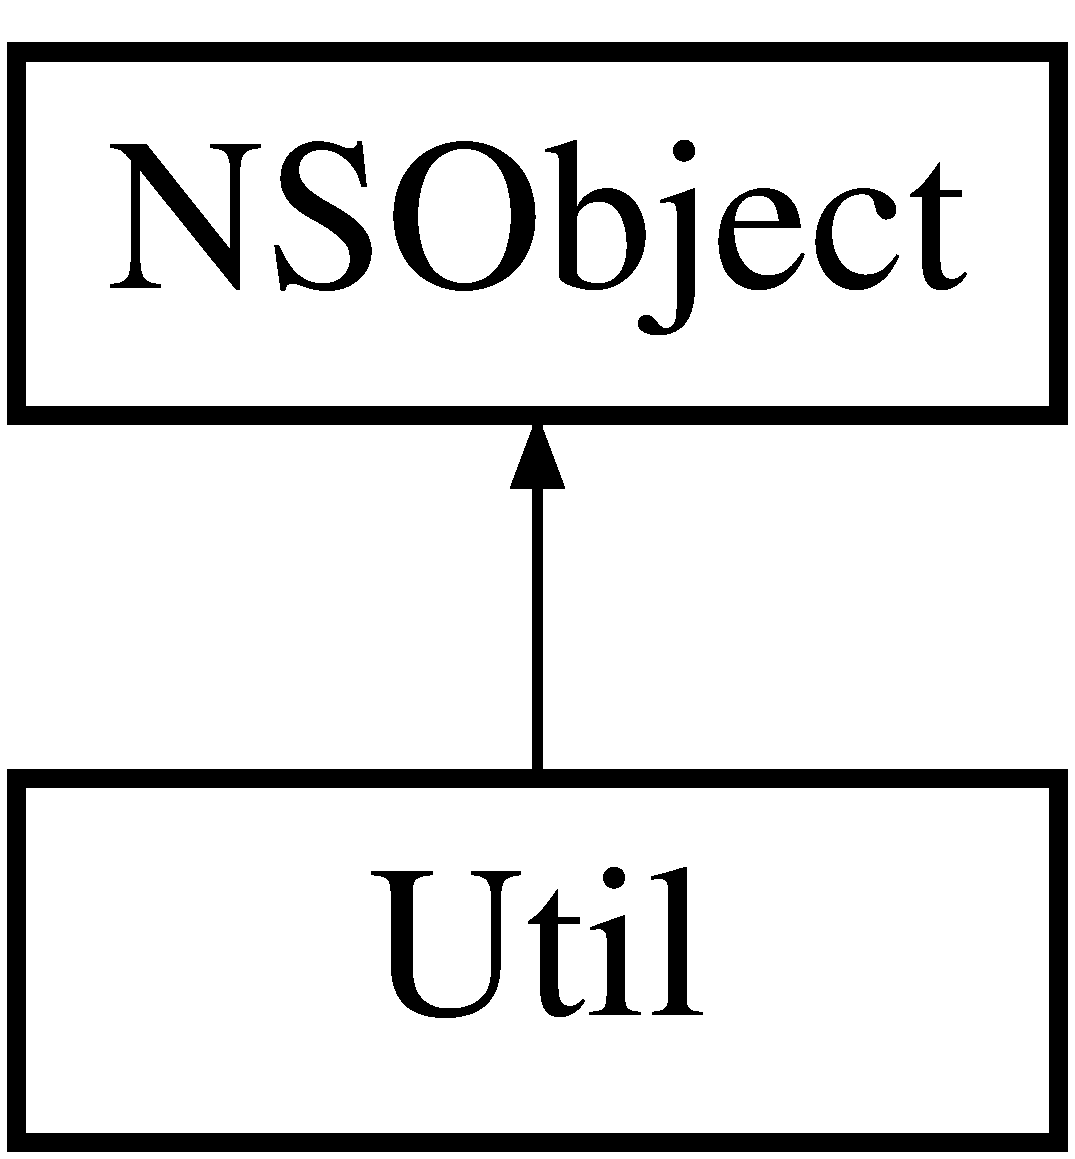
\includegraphics[height=2.000000cm]{interface_util}
\end{center}
\end{figure}
\subsection*{Class Methods}
\begin{DoxyCompactItemize}
\item 
(B\+O\+O\+L) + \hyperlink{interface_util_a344afa0140847ec221b1dbbcb04687f3}{is\+Network\+Available}
\item 
(U\+I\+Device\+Resolution) + \hyperlink{interface_util_ae8ae525e6770b696470ef18e3daaa2da}{current\+Resolution}
\item 
(B\+O\+O\+L) + \hyperlink{interface_util_ae29979775a0bc59108a2b8a6b47b0e2f}{is\+Running\+Oni\+Phone5}
\item 
(B\+O\+O\+L) + \hyperlink{interface_util_a1034ee0415e04b31875019f4c6bb96f1}{is\+Running\+Oni\+Phone}
\item 
(B\+O\+O\+L) + \hyperlink{interface_util_a65978baa276483a8bedff6b046eeeac1}{isi\+O\+S7\+Available}
\item 
(B\+O\+O\+L) + \hyperlink{interface_util_a27325e3210aa14c4aaafdf576329b828}{i\+Si\+O\+S8\+Available}
\item 
(N\+S\+String $\ast$) + \hyperlink{interface_util_a688fa2c31a825862e4059d4a37d87fa9}{M\+D5\+String\+:whether\+Up\+Case\+:}
\item 
(void) + \hyperlink{interface_util_a473a8c494766a9977139f3380efcd57e}{show\+Success}
\item 
(void) + \hyperlink{interface_util_a3bd6f354bd8aa2ec5bfc82009fcd026c}{make\+Toast\+:}
\item 
(M\+B\+Progress\+H\+U\+D $\ast$) + \hyperlink{interface_util_a2c46fb9ccbaf2328d22ec8b30fb08a7c}{show\+Progress\+Hud}
\item 
(N\+S\+String $\ast$) + \hyperlink{interface_util_a2b2160411cd3b13359ea0466b75d7c36}{current\+Time\+String}
\item 
(N\+S\+String $\ast$) + \hyperlink{interface_util_a0492aa8f02fc7d15ec1eb0ee3dbf9cc3}{current\+Time\+Without\+Space}
\item 
(B\+O\+O\+L) + \hyperlink{interface_util_a9e66070d674ed5d1750b70c6fbdedb9c}{check\+Phone\+Num\+Input\+:}
\item 
(void) + \hyperlink{interface_util_aecb38c60d70c7f77d578b7cc72056a6a}{push\+View\+Controller\+:navigation\+Controller\+:hide\+Tab\+Bar\+:}
\item 
(N\+S\+String $\ast$) + \hyperlink{interface_util_a07cf090688bfd3ed6cb0ba5d7ac5d6b1}{format\+Money\+:}
\item 
(N\+S\+String $\ast$) + \hyperlink{interface_util_af44a00916844095c45277978b3297f3c}{format\+Date\+:}
\item 
(N\+S\+String $\ast$) + \hyperlink{interface_util_acbee7aff4b5986e8fde1edf4d5cf0f9b}{format\+Date\+By\+Day\+:}
\item 
(N\+S\+String $\ast$) + \hyperlink{interface_util_a520c05b4d750450e210ed4b88fcda50e}{today}
\item 
(N\+S\+String $\ast$) + \hyperlink{interface_util_a45977a2f8e7932f43fd76a93513fb512}{get\+Time\+Relese\+:}
\item 
(void) + \hyperlink{interface_util_a61a4994395b62cd42c2faca10ae495da}{i\+O\+S7\+Style\+For\+U\+I\+Segment\+Underi\+O\+S6\+:normal\+Color\+:}
\item 
(void) + \hyperlink{interface_util_ab14c5f425ea917696d72ed2369a7c801}{i\+O\+S7\+Style\+For\+U\+I\+Bar\+Button\+Item\+Underi\+O\+S6\+:}
\item 
(void) + \hyperlink{interface_util_a7c0668508791ceb7e589895bc4ac5e01}{add\+Border\+For\+View\+:add\+Left\+:add\+Right\+:add\+Top\+:add\+Bottom\+:border\+Color\+:}
\item 
(N\+S\+String $\ast$) + \hyperlink{interface_util_a2d310eb623bc9a372a47941ff21873fe}{bool2\+String\+:}
\item 
(N\+S\+String $\ast$) + \hyperlink{interface_util_a0d99f08d8339ca006b2d3a3174daae4d}{int2\+String\+:}
\item 
(N\+S\+String $\ast$) + \hyperlink{interface_util_a1a65d58902cd896dade73f0f00a84c76}{float2\+String\+:}
\item 
(N\+S\+String $\ast$) + \hyperlink{interface_util_a2893806d2f63d616bb8f560a4dba2bdd}{combine\+String\+:with\+:}
\item 
(Carrier\+Type) + \hyperlink{interface_util_a32b4fde4fc895aa25ba998a9a13534d7}{carrier}
\item 
(void) + \hyperlink{interface_util_a99984eed9d29c144d0a19c6c47077045}{strikethrough\+Label\+:with\+Text\+:}
\item 
(void) + \hyperlink{interface_util_af39c1facf595566b0fc0c80bc9700279}{delete\+Back\+Title\+:}
\item 
(void) + \hyperlink{interface_util_ae0150c5515eafe256ea70a4952b0b156}{custom\+Button\+:enabled\+Color\+:disabled\+Color\+:whether\+Filleted\+Corner\+:}
\item 
(void) + \hyperlink{interface_util_a171e52b6e5e08297da84f8cfc50ee882}{set\+Extra\+Cell\+Line\+Hidden\+:}
\end{DoxyCompactItemize}


\subsection{Method Documentation}
\hypertarget{interface_util_a7c0668508791ceb7e589895bc4ac5e01}{\index{Util@{Util}!add\+Border\+For\+View\+:add\+Left\+:add\+Right\+:add\+Top\+:add\+Bottom\+:border\+Color\+:@{add\+Border\+For\+View\+:add\+Left\+:add\+Right\+:add\+Top\+:add\+Bottom\+:border\+Color\+:}}
\index{add\+Border\+For\+View\+:add\+Left\+:add\+Right\+:add\+Top\+:add\+Bottom\+:border\+Color\+:@{add\+Border\+For\+View\+:add\+Left\+:add\+Right\+:add\+Top\+:add\+Bottom\+:border\+Color\+:}!Util@{Util}}
\subsubsection[{add\+Border\+For\+View\+:add\+Left\+:add\+Right\+:add\+Top\+:add\+Bottom\+:border\+Color\+:}]{\setlength{\rightskip}{0pt plus 5cm}+ (void) add\+Border\+For\+View\+: 
\begin{DoxyParamCaption}
\item[{(U\+I\+View$\ast$)}]{view}
\item[{addLeft:(B\+O\+O\+L)}]{left}
\item[{addRight:(B\+O\+O\+L)}]{right}
\item[{addTop:(B\+O\+O\+L)}]{top}
\item[{addBottom:(B\+O\+O\+L)}]{bottom}
\item[{borderColor:(U\+I\+Color$\ast$)}]{color}
\end{DoxyParamCaption}
}}\label{interface_util_a7c0668508791ceb7e589895bc4ac5e01}
添加边框


\begin{DoxyParams}{Parameters}
{\em view} & \\
\hline
{\em left} & \\
\hline
{\em right} & \\
\hline
{\em top} & \\
\hline
{\em bottom} & \\
\hline
{\em color} & \\
\hline
\end{DoxyParams}
\hypertarget{interface_util_a2d310eb623bc9a372a47941ff21873fe}{\index{Util@{Util}!bool2\+String\+:@{bool2\+String\+:}}
\index{bool2\+String\+:@{bool2\+String\+:}!Util@{Util}}
\subsubsection[{bool2\+String\+:}]{\setlength{\rightskip}{0pt plus 5cm}+ (N\+S\+String $\ast$) bool2\+String\+: 
\begin{DoxyParamCaption}
\item[{(B\+O\+O\+L)}]{bool\+Value}
\end{DoxyParamCaption}
}}\label{interface_util_a2d310eb623bc9a372a47941ff21873fe}
bool转字符串


\begin{DoxyParams}{Parameters}
{\em bool\+Value} & \\
\hline
\end{DoxyParams}
\begin{DoxyReturn}{Returns}

\end{DoxyReturn}
\hypertarget{interface_util_a32b4fde4fc895aa25ba998a9a13534d7}{\index{Util@{Util}!carrier@{carrier}}
\index{carrier@{carrier}!Util@{Util}}
\subsubsection[{carrier}]{\setlength{\rightskip}{0pt plus 5cm}+ (Carrier\+Type) carrier 
\begin{DoxyParamCaption}
{}
\end{DoxyParamCaption}
}}\label{interface_util_a32b4fde4fc895aa25ba998a9a13534d7}
获取运营商信息

\begin{DoxyReturn}{Returns}

\end{DoxyReturn}
\hypertarget{interface_util_a9e66070d674ed5d1750b70c6fbdedb9c}{\index{Util@{Util}!check\+Phone\+Num\+Input\+:@{check\+Phone\+Num\+Input\+:}}
\index{check\+Phone\+Num\+Input\+:@{check\+Phone\+Num\+Input\+:}!Util@{Util}}
\subsubsection[{check\+Phone\+Num\+Input\+:}]{\setlength{\rightskip}{0pt plus 5cm}+ (B\+O\+O\+L) check\+Phone\+Num\+Input\+: 
\begin{DoxyParamCaption}
\item[{(N\+S\+String $\ast$)}]{phone}
\end{DoxyParamCaption}
}}\label{interface_util_a9e66070d674ed5d1750b70c6fbdedb9c}
检查电话号码格式


\begin{DoxyParams}{Parameters}
{\em phone} & \\
\hline
\end{DoxyParams}
\begin{DoxyReturn}{Returns}

\end{DoxyReturn}
\hypertarget{interface_util_a2893806d2f63d616bb8f560a4dba2bdd}{\index{Util@{Util}!combine\+String\+:with\+:@{combine\+String\+:with\+:}}
\index{combine\+String\+:with\+:@{combine\+String\+:with\+:}!Util@{Util}}
\subsubsection[{combine\+String\+:with\+:}]{\setlength{\rightskip}{0pt plus 5cm}+ (N\+S\+String $\ast$) combine\+String\+: 
\begin{DoxyParamCaption}
\item[{(N\+S\+String$\ast$)}]{string1}
\item[{with:(N\+S\+String$\ast$)}]{string2}
\end{DoxyParamCaption}
}}\label{interface_util_a2893806d2f63d616bb8f560a4dba2bdd}
拼接字符串


\begin{DoxyParams}{Parameters}
{\em string1} & \\
\hline
{\em string2} & \\
\hline
\end{DoxyParams}
\begin{DoxyReturn}{Returns}

\end{DoxyReturn}
\hypertarget{interface_util_ae8ae525e6770b696470ef18e3daaa2da}{\index{Util@{Util}!current\+Resolution@{current\+Resolution}}
\index{current\+Resolution@{current\+Resolution}!Util@{Util}}
\subsubsection[{current\+Resolution}]{\setlength{\rightskip}{0pt plus 5cm}+ (U\+I\+Device\+Resolution) current\+Resolution 
\begin{DoxyParamCaption}
{}
\end{DoxyParamCaption}
}}\label{interface_util_ae8ae525e6770b696470ef18e3daaa2da}
获取当前分辨率

\begin{DoxyReturn}{Returns}

\end{DoxyReturn}
\hypertarget{interface_util_a2b2160411cd3b13359ea0466b75d7c36}{\index{Util@{Util}!current\+Time\+String@{current\+Time\+String}}
\index{current\+Time\+String@{current\+Time\+String}!Util@{Util}}
\subsubsection[{current\+Time\+String}]{\setlength{\rightskip}{0pt plus 5cm}+ (N\+S\+String $\ast$) current\+Time\+String 
\begin{DoxyParamCaption}
{}
\end{DoxyParamCaption}
}}\label{interface_util_a2b2160411cd3b13359ea0466b75d7c36}
获取当前时间格式化字符串 2016-\/01-\/07 13\+:36\+:38 形式

\begin{DoxyReturn}{Returns}

\end{DoxyReturn}
\hypertarget{interface_util_a0492aa8f02fc7d15ec1eb0ee3dbf9cc3}{\index{Util@{Util}!current\+Time\+Without\+Space@{current\+Time\+Without\+Space}}
\index{current\+Time\+Without\+Space@{current\+Time\+Without\+Space}!Util@{Util}}
\subsubsection[{current\+Time\+Without\+Space}]{\setlength{\rightskip}{0pt plus 5cm}+ (N\+S\+String $\ast$) current\+Time\+Without\+Space 
\begin{DoxyParamCaption}
{}
\end{DoxyParamCaption}
}}\label{interface_util_a0492aa8f02fc7d15ec1eb0ee3dbf9cc3}
获取当前时间格式化字符串,无空格 20160107\+\_\+13\+\_\+36\+\_\+38 形式

\begin{DoxyReturn}{Returns}

\end{DoxyReturn}
\hypertarget{interface_util_ae0150c5515eafe256ea70a4952b0b156}{\index{Util@{Util}!custom\+Button\+:enabled\+Color\+:disabled\+Color\+:whether\+Filleted\+Corner\+:@{custom\+Button\+:enabled\+Color\+:disabled\+Color\+:whether\+Filleted\+Corner\+:}}
\index{custom\+Button\+:enabled\+Color\+:disabled\+Color\+:whether\+Filleted\+Corner\+:@{custom\+Button\+:enabled\+Color\+:disabled\+Color\+:whether\+Filleted\+Corner\+:}!Util@{Util}}
\subsubsection[{custom\+Button\+:enabled\+Color\+:disabled\+Color\+:whether\+Filleted\+Corner\+:}]{\setlength{\rightskip}{0pt plus 5cm}+ (void) custom\+Button\+: 
\begin{DoxyParamCaption}
\item[{(U\+I\+Button$\ast$)}]{button}
\item[{enabledColor:(N\+S\+Integer)}]{enabled\+Color}
\item[{disabledColor:(N\+S\+Integer)}]{disabled\+Color}
\item[{whetherFilletedCorner:(B\+O\+O\+L)}]{has\+Filleted\+Corner}
\end{DoxyParamCaption}
}}\label{interface_util_ae0150c5515eafe256ea70a4952b0b156}
自定义圆角button的背景色


\begin{DoxyParams}{Parameters}
{\em button} & \\
\hline
{\em enabled\+Color} & button启用时的颜色 16进制 \\
\hline
{\em disabled\+Color} & button禁用时的颜色 16进制 \\
\hline
{\em has\+Filleted\+Corner} & 是否需要圆角 \\
\hline
\end{DoxyParams}
\hypertarget{interface_util_af39c1facf595566b0fc0c80bc9700279}{\index{Util@{Util}!delete\+Back\+Title\+:@{delete\+Back\+Title\+:}}
\index{delete\+Back\+Title\+:@{delete\+Back\+Title\+:}!Util@{Util}}
\subsubsection[{delete\+Back\+Title\+:}]{\setlength{\rightskip}{0pt plus 5cm}+ (void) delete\+Back\+Title\+: 
\begin{DoxyParamCaption}
\item[{(U\+I\+Navigation\+Item$\ast$)}]{navigation\+Item}
\end{DoxyParamCaption}
}}\label{interface_util_af39c1facf595566b0fc0c80bc9700279}
删除返回按钮边上的文字,注意,这是删除下一个页面的返回按钮的文字,对当前页面无效


\begin{DoxyParams}{Parameters}
{\em navigation\+Item} & \\
\hline
\end{DoxyParams}
\hypertarget{interface_util_a1a65d58902cd896dade73f0f00a84c76}{\index{Util@{Util}!float2\+String\+:@{float2\+String\+:}}
\index{float2\+String\+:@{float2\+String\+:}!Util@{Util}}
\subsubsection[{float2\+String\+:}]{\setlength{\rightskip}{0pt plus 5cm}+ (N\+S\+String $\ast$) float2\+String\+: 
\begin{DoxyParamCaption}
\item[{(float)}]{float\+Value}
\end{DoxyParamCaption}
}}\label{interface_util_a1a65d58902cd896dade73f0f00a84c76}
浮点型转字符串


\begin{DoxyParams}{Parameters}
{\em float\+Value} & \\
\hline
\end{DoxyParams}
\begin{DoxyReturn}{Returns}

\end{DoxyReturn}
\hypertarget{interface_util_af44a00916844095c45277978b3297f3c}{\index{Util@{Util}!format\+Date\+:@{format\+Date\+:}}
\index{format\+Date\+:@{format\+Date\+:}!Util@{Util}}
\subsubsection[{format\+Date\+:}]{\setlength{\rightskip}{0pt plus 5cm}+ (N\+S\+String $\ast$) format\+Date\+: 
\begin{DoxyParamCaption}
\item[{(long)}]{time\+Mills}
\end{DoxyParamCaption}
}}\label{interface_util_af44a00916844095c45277978b3297f3c}
格式化日期显示 yyyy-\/\+M\+M-\/dd H\+H\+:mm\+:ss


\begin{DoxyParams}{Parameters}
{\em time\+Mills} & \\
\hline
\end{DoxyParams}
\begin{DoxyReturn}{Returns}

\end{DoxyReturn}
\hypertarget{interface_util_acbee7aff4b5986e8fde1edf4d5cf0f9b}{\index{Util@{Util}!format\+Date\+By\+Day\+:@{format\+Date\+By\+Day\+:}}
\index{format\+Date\+By\+Day\+:@{format\+Date\+By\+Day\+:}!Util@{Util}}
\subsubsection[{format\+Date\+By\+Day\+:}]{\setlength{\rightskip}{0pt plus 5cm}+ (N\+S\+String $\ast$) format\+Date\+By\+Day\+: 
\begin{DoxyParamCaption}
\item[{(N\+S\+String$\ast$)}]{formatted\+Date\+By\+Seconds}
\end{DoxyParamCaption}
}}\label{interface_util_acbee7aff4b5986e8fde1edf4d5cf0f9b}
格式化日期显示 yyyy-\/\+M\+M-\/dd


\begin{DoxyParams}{Parameters}
{\em formatted\+Date\+By\+Seconds} & \\
\hline
\end{DoxyParams}
\begin{DoxyReturn}{Returns}

\end{DoxyReturn}
\hypertarget{interface_util_a07cf090688bfd3ed6cb0ba5d7ac5d6b1}{\index{Util@{Util}!format\+Money\+:@{format\+Money\+:}}
\index{format\+Money\+:@{format\+Money\+:}!Util@{Util}}
\subsubsection[{format\+Money\+:}]{\setlength{\rightskip}{0pt plus 5cm}+ (N\+S\+String $\ast$) format\+Money\+: 
\begin{DoxyParamCaption}
\item[{(float)}]{money}
\end{DoxyParamCaption}
}}\label{interface_util_a07cf090688bfd3ed6cb0ba5d7ac5d6b1}
格式化价格显示 例如:¥1.00


\begin{DoxyParams}{Parameters}
{\em money} & \\
\hline
\end{DoxyParams}
\begin{DoxyReturn}{Returns}

\end{DoxyReturn}
\hypertarget{interface_util_a45977a2f8e7932f43fd76a93513fb512}{\index{Util@{Util}!get\+Time\+Relese\+:@{get\+Time\+Relese\+:}}
\index{get\+Time\+Relese\+:@{get\+Time\+Relese\+:}!Util@{Util}}
\subsubsection[{get\+Time\+Relese\+:}]{\setlength{\rightskip}{0pt plus 5cm}+ (N\+S\+String $\ast$) get\+Time\+Relese\+: 
\begin{DoxyParamCaption}
\item[{(N\+S\+String $\ast$)}]{timenode}
\end{DoxyParamCaption}
}}\label{interface_util_a45977a2f8e7932f43fd76a93513fb512}
求时间差 0日0时0分0秒结束 形式


\begin{DoxyParams}{Parameters}
{\em timenode} & \\
\hline
\end{DoxyParams}
\begin{DoxyReturn}{Returns}

\end{DoxyReturn}
\hypertarget{interface_util_a0d99f08d8339ca006b2d3a3174daae4d}{\index{Util@{Util}!int2\+String\+:@{int2\+String\+:}}
\index{int2\+String\+:@{int2\+String\+:}!Util@{Util}}
\subsubsection[{int2\+String\+:}]{\setlength{\rightskip}{0pt plus 5cm}+ (N\+S\+String $\ast$) int2\+String\+: 
\begin{DoxyParamCaption}
\item[{(int)}]{int\+Value}
\end{DoxyParamCaption}
}}\label{interface_util_a0d99f08d8339ca006b2d3a3174daae4d}
整型转字符串


\begin{DoxyParams}{Parameters}
{\em int\+Value} & \\
\hline
\end{DoxyParams}
\begin{DoxyReturn}{Returns}

\end{DoxyReturn}
\hypertarget{interface_util_ab14c5f425ea917696d72ed2369a7c801}{\index{Util@{Util}!i\+O\+S7\+Style\+For\+U\+I\+Bar\+Button\+Item\+Underi\+O\+S6\+:@{i\+O\+S7\+Style\+For\+U\+I\+Bar\+Button\+Item\+Underi\+O\+S6\+:}}
\index{i\+O\+S7\+Style\+For\+U\+I\+Bar\+Button\+Item\+Underi\+O\+S6\+:@{i\+O\+S7\+Style\+For\+U\+I\+Bar\+Button\+Item\+Underi\+O\+S6\+:}!Util@{Util}}
\subsubsection[{i\+O\+S7\+Style\+For\+U\+I\+Bar\+Button\+Item\+Underi\+O\+S6\+:}]{\setlength{\rightskip}{0pt plus 5cm}+ (void) i\+O\+S7\+Style\+For\+U\+I\+Bar\+Button\+Item\+Underi\+O\+S6\+: 
\begin{DoxyParamCaption}
\item[{(N\+S\+String$\ast$)}]{back\+Image\+Name}
\end{DoxyParamCaption}
}}\label{interface_util_ab14c5f425ea917696d72ed2369a7c801}
i\+O\+S6下的nav的返回按钮的扁平化


\begin{DoxyParams}{Parameters}
{\em back\+Image\+Name} & 回退图片的名字 \\
\hline
\end{DoxyParams}
\hypertarget{interface_util_a61a4994395b62cd42c2faca10ae495da}{\index{Util@{Util}!i\+O\+S7\+Style\+For\+U\+I\+Segment\+Underi\+O\+S6\+:normal\+Color\+:@{i\+O\+S7\+Style\+For\+U\+I\+Segment\+Underi\+O\+S6\+:normal\+Color\+:}}
\index{i\+O\+S7\+Style\+For\+U\+I\+Segment\+Underi\+O\+S6\+:normal\+Color\+:@{i\+O\+S7\+Style\+For\+U\+I\+Segment\+Underi\+O\+S6\+:normal\+Color\+:}!Util@{Util}}
\subsubsection[{i\+O\+S7\+Style\+For\+U\+I\+Segment\+Underi\+O\+S6\+:normal\+Color\+:}]{\setlength{\rightskip}{0pt plus 5cm}+ (void) i\+O\+S7\+Style\+For\+U\+I\+Segment\+Underi\+O\+S6\+: 
\begin{DoxyParamCaption}
\item[{(U\+I\+Color$\ast$)}]{selected\+Color}
\item[{normalColor:(U\+I\+Color$\ast$)}]{normal\+Color}
\end{DoxyParamCaption}
}}\label{interface_util_a61a4994395b62cd42c2faca10ae495da}
i\+O\+S6下\+U\+I\+Segment的扁平化


\begin{DoxyParams}{Parameters}
{\em selected\+Color} & 选中时的背景颜色 \\
\hline
{\em normal\+Color} & 未选中时的背景颜色 \\
\hline
\end{DoxyParams}
\hypertarget{interface_util_a65978baa276483a8bedff6b046eeeac1}{\index{Util@{Util}!isi\+O\+S7\+Available@{isi\+O\+S7\+Available}}
\index{isi\+O\+S7\+Available@{isi\+O\+S7\+Available}!Util@{Util}}
\subsubsection[{isi\+O\+S7\+Available}]{\setlength{\rightskip}{0pt plus 5cm}+ (B\+O\+O\+L) isi\+O\+S7\+Available 
\begin{DoxyParamCaption}
{}
\end{DoxyParamCaption}
}}\label{interface_util_a65978baa276483a8bedff6b046eeeac1}
是否是i\+O\+S7.0以上

\begin{DoxyReturn}{Returns}

\end{DoxyReturn}
\hypertarget{interface_util_a27325e3210aa14c4aaafdf576329b828}{\index{Util@{Util}!i\+Si\+O\+S8\+Available@{i\+Si\+O\+S8\+Available}}
\index{i\+Si\+O\+S8\+Available@{i\+Si\+O\+S8\+Available}!Util@{Util}}
\subsubsection[{i\+Si\+O\+S8\+Available}]{\setlength{\rightskip}{0pt plus 5cm}+ (B\+O\+O\+L) i\+Si\+O\+S8\+Available 
\begin{DoxyParamCaption}
{}
\end{DoxyParamCaption}
}}\label{interface_util_a27325e3210aa14c4aaafdf576329b828}
是否是i\+O\+S8.0以上

\begin{DoxyReturn}{Returns}

\end{DoxyReturn}
\hypertarget{interface_util_a344afa0140847ec221b1dbbcb04687f3}{\index{Util@{Util}!is\+Network\+Available@{is\+Network\+Available}}
\index{is\+Network\+Available@{is\+Network\+Available}!Util@{Util}}
\subsubsection[{is\+Network\+Available}]{\setlength{\rightskip}{0pt plus 5cm}+ (B\+O\+O\+L) is\+Network\+Available 
\begin{DoxyParamCaption}
{}
\end{DoxyParamCaption}
}}\label{interface_util_a344afa0140847ec221b1dbbcb04687f3}
判断是否有网络 \begin{DoxyRefDesc}{Deprecated}
\item[\hyperlink{deprecated__deprecated000001}{Deprecated}]直接使用\mbox{[}\mbox{[}Cloud\+Client shared\+Instance\mbox{]} is\+Reachable\mbox{]}; \begin{DoxyReturn}{Returns}

\end{DoxyReturn}
\end{DoxyRefDesc}
S\+C\+Network\+Reachability\+Ref\+: 用来保存创建测试连接返回的引用

S\+C\+Network\+Reachability\+Create\+With\+Address\+: 根据传入的地址测试连接. 第一个参数可以为\+N\+U\+L\+L或k\+C\+F\+Allocator\+Default 第二个参数为需要测试连接的\+I\+P地址,当为0.0.\+0.\+0时则可以查询本机的网络连接状态. 同时返回一个引用必须在用完后释放. P\+S\+: S\+C\+Network\+Reachability\+Create\+With\+Name\+: 这个是根据传入的网址测试连接, 第二个参数比如为\char`\"{}www.\+apple.\+com\char`\"{},其他和上一个一样.

S\+C\+Network\+Reachability\+Get\+Flags\+: 这个函数用来获得测试连接的状态, 第一个参数为之前建立的测试连接的引用, 第二个参数用来保存获得的状态, 如果能获得状态则返回\+T\+R\+U\+E,否则返回\+F\+A\+L\+S\+E

k\+S\+C\+Network\+Reachability\+Flags\+Reachable\+: 能够连接网络 k\+S\+C\+Network\+Reachability\+Flags\+Connection\+Required\+: 能够连接网络,但是首先得建立连接过程 k\+S\+C\+Network\+Reachability\+Flags\+Is\+W\+W\+A\+N\+: 判断是否通过蜂窝网覆盖的连接, 比如\+E\+D\+G\+E,G\+P\+R\+S或者目前的3\+G.\+主要是区别通过\+Wi\+Fi的连接.\hypertarget{interface_util_a1034ee0415e04b31875019f4c6bb96f1}{\index{Util@{Util}!is\+Running\+Oni\+Phone@{is\+Running\+Oni\+Phone}}
\index{is\+Running\+Oni\+Phone@{is\+Running\+Oni\+Phone}!Util@{Util}}
\subsubsection[{is\+Running\+Oni\+Phone}]{\setlength{\rightskip}{0pt plus 5cm}+ (B\+O\+O\+L) is\+Running\+Oni\+Phone 
\begin{DoxyParamCaption}
{}
\end{DoxyParamCaption}
}}\label{interface_util_a1034ee0415e04b31875019f4c6bb96f1}
是否是i\+Phone

\begin{DoxyReturn}{Returns}

\end{DoxyReturn}
\hypertarget{interface_util_ae29979775a0bc59108a2b8a6b47b0e2f}{\index{Util@{Util}!is\+Running\+Oni\+Phone5@{is\+Running\+Oni\+Phone5}}
\index{is\+Running\+Oni\+Phone5@{is\+Running\+Oni\+Phone5}!Util@{Util}}
\subsubsection[{is\+Running\+Oni\+Phone5}]{\setlength{\rightskip}{0pt plus 5cm}+ (B\+O\+O\+L) is\+Running\+Oni\+Phone5 
\begin{DoxyParamCaption}
{}
\end{DoxyParamCaption}
}}\label{interface_util_ae29979775a0bc59108a2b8a6b47b0e2f}
是否是i\+Phone5

\begin{DoxyReturn}{Returns}

\end{DoxyReturn}
\hypertarget{interface_util_a3bd6f354bd8aa2ec5bfc82009fcd026c}{\index{Util@{Util}!make\+Toast\+:@{make\+Toast\+:}}
\index{make\+Toast\+:@{make\+Toast\+:}!Util@{Util}}
\subsubsection[{make\+Toast\+:}]{\setlength{\rightskip}{0pt plus 5cm}+ (void) make\+Toast\+: 
\begin{DoxyParamCaption}
\item[{(N\+S\+String $\ast$)}]{message}
\end{DoxyParamCaption}
}}\label{interface_util_a3bd6f354bd8aa2ec5bfc82009fcd026c}
弹出消息提示,1.5秒后消失


\begin{DoxyParams}{Parameters}
{\em message} & 提示内容\\
\hline
\end{DoxyParams}
弹出文字提示 \hypertarget{interface_util_a688fa2c31a825862e4059d4a37d87fa9}{\index{Util@{Util}!M\+D5\+String\+:whether\+Up\+Case\+:@{M\+D5\+String\+:whether\+Up\+Case\+:}}
\index{M\+D5\+String\+:whether\+Up\+Case\+:@{M\+D5\+String\+:whether\+Up\+Case\+:}!Util@{Util}}
\subsubsection[{M\+D5\+String\+:whether\+Up\+Case\+:}]{\setlength{\rightskip}{0pt plus 5cm}+ (N\+S\+String $\ast$) M\+D5\+String\+: 
\begin{DoxyParamCaption}
\item[{(N\+S\+String $\ast$)}]{string}
\item[{whetherUpCase:(B\+O\+O\+L)}]{to\+Up\+Case}
\end{DoxyParamCaption}
}}\label{interface_util_a688fa2c31a825862e4059d4a37d87fa9}
获取\+String的\+M\+D5值,可以设定大写或小写


\begin{DoxyParams}{Parameters}
{\em string} & 待加密字符串 \\
\hline
{\em to\+Up\+Case} & 是否大写\\
\hline
\end{DoxyParams}
\begin{DoxyReturn}{Returns}

\end{DoxyReturn}
字符串\+M\+D5加密 \hypertarget{interface_util_aecb38c60d70c7f77d578b7cc72056a6a}{\index{Util@{Util}!push\+View\+Controller\+:navigation\+Controller\+:hide\+Tab\+Bar\+:@{push\+View\+Controller\+:navigation\+Controller\+:hide\+Tab\+Bar\+:}}
\index{push\+View\+Controller\+:navigation\+Controller\+:hide\+Tab\+Bar\+:@{push\+View\+Controller\+:navigation\+Controller\+:hide\+Tab\+Bar\+:}!Util@{Util}}
\subsubsection[{push\+View\+Controller\+:navigation\+Controller\+:hide\+Tab\+Bar\+:}]{\setlength{\rightskip}{0pt plus 5cm}+ (void) push\+View\+Controller\+: 
\begin{DoxyParamCaption}
\item[{(Class)}]{view\+Controller\+Class}
\item[{navigationController:(U\+I\+Navigation\+Controller$\ast$)}]{navigation\+Controller}
\item[{hideTabBar:(B\+O\+O\+L)}]{hide\+Tab\+Bar}
\end{DoxyParamCaption}
}}\label{interface_util_aecb38c60d70c7f77d578b7cc72056a6a}
push 一个指定的\+View\+Controller


\begin{DoxyParams}{Parameters}
{\em view\+Controller\+Class} & 目标viewcontroller类 \\
\hline
{\em navigation\+Controller} & 导航栏控制器 \\
\hline
{\em hide\+Tab\+Bar} & 是否隐藏tabbar \\
\hline
\end{DoxyParams}
\hypertarget{interface_util_a171e52b6e5e08297da84f8cfc50ee882}{\index{Util@{Util}!set\+Extra\+Cell\+Line\+Hidden\+:@{set\+Extra\+Cell\+Line\+Hidden\+:}}
\index{set\+Extra\+Cell\+Line\+Hidden\+:@{set\+Extra\+Cell\+Line\+Hidden\+:}!Util@{Util}}
\subsubsection[{set\+Extra\+Cell\+Line\+Hidden\+:}]{\setlength{\rightskip}{0pt plus 5cm}+ (void) set\+Extra\+Cell\+Line\+Hidden\+: 
\begin{DoxyParamCaption}
\item[{(U\+I\+Table\+View $\ast$)}]{table\+View}
\end{DoxyParamCaption}
}}\label{interface_util_a171e52b6e5e08297da84f8cfc50ee882}
隐藏tableview的横线(无数据)


\begin{DoxyParams}{Parameters}
{\em table\+View} & \\
\hline
\end{DoxyParams}
\hypertarget{interface_util_a2c46fb9ccbaf2328d22ec8b30fb08a7c}{\index{Util@{Util}!show\+Progress\+Hud@{show\+Progress\+Hud}}
\index{show\+Progress\+Hud@{show\+Progress\+Hud}!Util@{Util}}
\subsubsection[{show\+Progress\+Hud}]{\setlength{\rightskip}{0pt plus 5cm}+ (M\+B\+Progress\+H\+U\+D $\ast$) show\+Progress\+Hud 
\begin{DoxyParamCaption}
{}
\end{DoxyParamCaption}
}}\label{interface_util_a2c46fb9ccbaf2328d22ec8b30fb08a7c}
显示正在加载提示

\begin{DoxyReturn}{Returns}

\end{DoxyReturn}
\hypertarget{interface_util_a473a8c494766a9977139f3380efcd57e}{\index{Util@{Util}!show\+Success@{show\+Success}}
\index{show\+Success@{show\+Success}!Util@{Util}}
\subsubsection[{show\+Success}]{\setlength{\rightskip}{0pt plus 5cm}+ (void) show\+Success 
\begin{DoxyParamCaption}
{}
\end{DoxyParamCaption}
}}\label{interface_util_a473a8c494766a9977139f3380efcd57e}
成功提示


\begin{DoxyParams}{Parameters}
{\em message} & \\
\hline
\end{DoxyParams}
\hypertarget{interface_util_a99984eed9d29c144d0a19c6c47077045}{\index{Util@{Util}!strikethrough\+Label\+:with\+Text\+:@{strikethrough\+Label\+:with\+Text\+:}}
\index{strikethrough\+Label\+:with\+Text\+:@{strikethrough\+Label\+:with\+Text\+:}!Util@{Util}}
\subsubsection[{strikethrough\+Label\+:with\+Text\+:}]{\setlength{\rightskip}{0pt plus 5cm}+ (void) strikethrough\+Label\+: 
\begin{DoxyParamCaption}
\item[{(U\+I\+Label$\ast$)}]{label}
\item[{withText:(N\+S\+String$\ast$)}]{text}
\end{DoxyParamCaption}
}}\label{interface_util_a99984eed9d29c144d0a19c6c47077045}
实现富文本显示,效果是在显示的文本上增加一条划线


\begin{DoxyParams}{Parameters}
{\em label} & 目标label \\
\hline
{\em text} & 文本 \\
\hline
\end{DoxyParams}
\hypertarget{interface_util_a520c05b4d750450e210ed4b88fcda50e}{\index{Util@{Util}!today@{today}}
\index{today@{today}!Util@{Util}}
\subsubsection[{today}]{\setlength{\rightskip}{0pt plus 5cm}+ (N\+S\+String $\ast$) today 
\begin{DoxyParamCaption}
{}
\end{DoxyParamCaption}
}}\label{interface_util_a520c05b4d750450e210ed4b88fcda50e}
今天,2014-\/09-\/09 形式

\begin{DoxyReturn}{Returns}

\end{DoxyReturn}


The documentation for this class was generated from the following files\+:\begin{DoxyCompactItemize}
\item 
Util/Util.\+h\item 
Util/Util.\+m\end{DoxyCompactItemize}

\hypertarget{class_z_l_g_t_m_base64}{\section{Z\+L\+G\+T\+M\+Base64 Class Reference}
\label{class_z_l_g_t_m_base64}\index{Z\+L\+G\+T\+M\+Base64@{Z\+L\+G\+T\+M\+Base64}}
}


The documentation for this class was generated from the following file\+:\begin{DoxyCompactItemize}
\item 
Base64/Z\+L\+G\+T\+M\+Base64.\+m\end{DoxyCompactItemize}

\hypertarget{category_z_l_g_t_m_base64_07_private_methods_08}{\section{Z\+L\+G\+T\+M\+Base64(Private\+Methods) Category Reference}
\label{category_z_l_g_t_m_base64_07_private_methods_08}\index{Z\+L\+G\+T\+M\+Base64(\+Private\+Methods)@{Z\+L\+G\+T\+M\+Base64(\+Private\+Methods)}}
}
\subsection*{Class Methods}
\begin{DoxyCompactItemize}
\item 
\hypertarget{category_z_l_g_t_m_base64_07_private_methods_08_a5fc4c3bf3f30c7dfd9940d6446f8b854}{(N\+S\+Data $\ast$) + {\bfseries base\+Encode\+:length\+:charset\+:padded\+:}}\label{category_z_l_g_t_m_base64_07_private_methods_08_a5fc4c3bf3f30c7dfd9940d6446f8b854}

\item 
\hypertarget{category_z_l_g_t_m_base64_07_private_methods_08_aa48d690bcbc7cc31f4ceb8be724344aa}{(N\+S\+Data $\ast$) + {\bfseries base\+Decode\+:length\+:charset\+:require\+Padding\+:}}\label{category_z_l_g_t_m_base64_07_private_methods_08_aa48d690bcbc7cc31f4ceb8be724344aa}

\item 
\hypertarget{category_z_l_g_t_m_base64_07_private_methods_08_ac56c08867c5eb64ef56a02461668d771}{(N\+S\+U\+Integer) + {\bfseries base\+Encode\+:src\+Len\+:dest\+Bytes\+:dest\+Len\+:charset\+:padded\+:}}\label{category_z_l_g_t_m_base64_07_private_methods_08_ac56c08867c5eb64ef56a02461668d771}

\item 
\hypertarget{category_z_l_g_t_m_base64_07_private_methods_08_a85d6cfd028d395197fcc1b453e4ae583}{(N\+S\+U\+Integer) + {\bfseries base\+Decode\+:src\+Len\+:dest\+Bytes\+:dest\+Len\+:charset\+:require\+Padding\+:}}\label{category_z_l_g_t_m_base64_07_private_methods_08_a85d6cfd028d395197fcc1b453e4ae583}

\end{DoxyCompactItemize}


The documentation for this category was generated from the following file\+:\begin{DoxyCompactItemize}
\item 
Base64/Z\+L\+G\+T\+M\+Base64.\+m\end{DoxyCompactItemize}

\hypertarget{interface_z_l_object_button}{\section{Z\+L\+Object\+Button Class Reference}
\label{interface_z_l_object_button}\index{Z\+L\+Object\+Button@{Z\+L\+Object\+Button}}
}
Inheritance diagram for Z\+L\+Object\+Button\+:\begin{figure}[H]
\begin{center}
\leavevmode
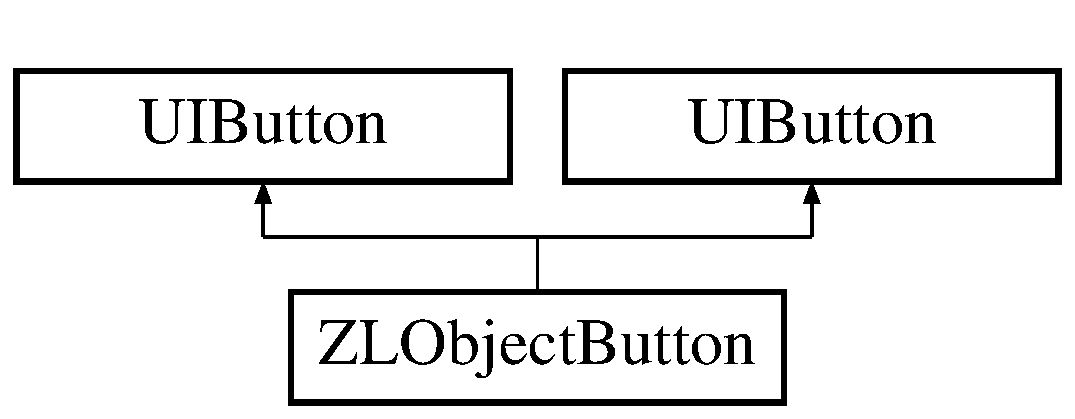
\includegraphics[height=2.000000cm]{interface_z_l_object_button}
\end{center}
\end{figure}
\subsection*{Properties}
\begin{DoxyCompactItemize}
\item 
\hypertarget{interface_z_l_object_button_acb703217b365373b42a35836db3e6898}{id {\bfseries object}}\label{interface_z_l_object_button_acb703217b365373b42a35836db3e6898}

\end{DoxyCompactItemize}


The documentation for this class was generated from the following file\+:\begin{DoxyCompactItemize}
\item 
Util/Z\+L\+Object\+Button.\+h\end{DoxyCompactItemize}

\hypertarget{interface_z_l_object_text_field}{\section{Z\+L\+Object\+Text\+Field Class Reference}
\label{interface_z_l_object_text_field}\index{Z\+L\+Object\+Text\+Field@{Z\+L\+Object\+Text\+Field}}
}
Inheritance diagram for Z\+L\+Object\+Text\+Field\+:\begin{figure}[H]
\begin{center}
\leavevmode
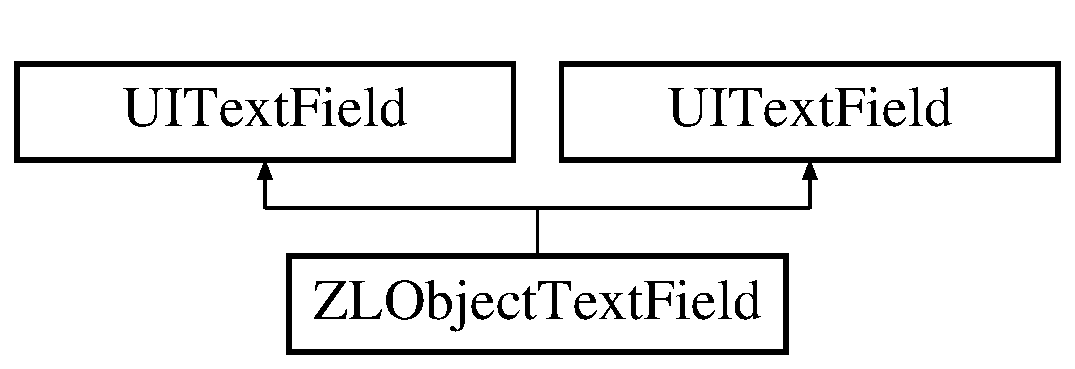
\includegraphics[height=2.000000cm]{interface_z_l_object_text_field}
\end{center}
\end{figure}
\subsection*{Properties}
\begin{DoxyCompactItemize}
\item 
\hypertarget{interface_z_l_object_text_field_afa177c78ec7c989d4f9b30c46b03b5c1}{id {\bfseries object}}\label{interface_z_l_object_text_field_afa177c78ec7c989d4f9b30c46b03b5c1}

\end{DoxyCompactItemize}


The documentation for this class was generated from the following file\+:\begin{DoxyCompactItemize}
\item 
Util/Z\+L\+Object\+Text\+Field.\+h\end{DoxyCompactItemize}

%--- End generated contents ---

% Index
\newpage
\phantomsection
\addcontentsline{toc}{chapter}{Index}
\printindex

\end{document}
